\documentclass[11pt, english, singlespacing, liststotoc, toctotoc, headsepline, chapterinoneline]{ClassThesis} % The class file specifying the document structure

\usepackage[utf8]{inputenc} % Required for inputting international characters
\usepackage[T1]{fontenc} % Output font encoding for international characters

%\usepackage{mathpazo} % Use the Palatino font by default
\usepackage{mathptmx}
%\usepackage{stix} % tipo de fuente
\usepackage{microtype} 
\usepackage{datetime}
\usepackage{comment}

\usepackage{mathtools} % símbolos extensibles (contiene amsmath)
\usepackage{amssymb} % símbolos matemáticos
\usepackage{amsthm} % para teoremas, lemas, ...
\usepackage{mathrsfs} % para usar \mathscr{}
\usepackage{tensor} % índices en cualquier lado
\usepackage{cancel} % tachar
\usepackage{dsfont} % usar fuente bbm en modo mates (para poner la identidad en vd)

\usepackage{array} % arrays
\usepackage{multirow} % redimensionar, unir celdas, ...
\usepackage{blkarray} % arrays en bloques
\usepackage{footnote} % notas a pie de pagina
\usepackage{multicol}

\usepackage{float} % para figuras (las fija, [H], ...)
\usepackage{chngcntr}
\counterwithout{figure}{chapter}

\renewcommand{\theenumi}{\roman{enumi}}
\renewcommand{\thefigure}{\Roman{figure}} 
\renewcommand{\thesubfigure}{\Alph{subfigure}}
\newcommand\diagram[2]{\schema{\schemabox{#1}}{\schemabox{#2}}}
\newtheorem{theorem}{Teorema}[section]
\newtheorem{example}{Ejemplo}[section]
\newtheorem{lemma}{Lema}
\newtheorem{definition}{Definición}[section]
\newtheorem{comentario}{Comentario}[section]
\def\proof{\paragraph{Demostraci\'on:\\}}
\def\endproof{\hfill$\blacksquare$}
\DeclareMathOperator*{\argmax}{arg\,max}


% chktex-file 12
% chktex-file 13
% chktex-file 44
\usepackage{tcolorbox}
\usepackage{enumitem}
\usepackage{verbatim}
\usepackage{pdfpages}
\usepackage[backend=bibtex, style=authoryear, natbib=true, maxcitenames=2, maxbibnames=20, minbibnames=1]{biblatex} % Use the bibtex backend with the authoryear citation style (which resembles APA) % sorting=none for citation order
\addbibresource{references.bib} % The filename of the bibliography
\setlength\bibitemsep{1.5\itemsep}

\usepackage[autostyle=true]{csquotes} % Required to generate language-dependent quotes in the bibliography

%----------------------------------------------------------------------------------------
%	MARGIN SETTINGS
%----------------------------------------------------------------------------------------

\geometry{
	paper=a4paper, % Change to letterpaper for US letter
	inner=2.5cm, % Inner margin
	outer=3.8cm, % Outer margin
	bindingoffset=.5cm, % Binding offset
	top=1.5cm, % Top margin
	bottom=1.5cm, % Bottom margin
	%showframe, % Uncomment to show how the type block is set on the page
}

%----------------------------------------------------------------------------------------
%	THESIS INFORMATION
%----------------------------------------------------------------------------------------

\thesistitle{Aprendizaje estadístico} % \ttitle
\supervisor{Jose Ameijeiras Alonso \\ Manuel Mucientes Molina} % \supname
\examiner{} % \examname
\degree{Master en Tecnoloxías de Análise \\ de Datos Masivos: Big Data} % \degreename
\author{Luis Ardévol Mesa} % \authorname
\addresses{} % \addressname

\subject{} % Subject area, print it elsewhere with \subjectname
\keywords{} %\keywordnames
\university{Universidad de Santiago de Compostela} % \univname
\department{} % \deptname
\group{} % \groupname
\faculty{Escola Técnica Superior de Enxeñaría} % \facname

\AtBeginDocument{
\hypersetup{pdftitle=\ttitle} % Set the PDF's title to your title
\hypersetup{pdfauthor=\authorname} % Set the PDF's author to your name
\hypersetup{pdfkeywords=\keywordnames} % Set the PDF's keywords to your keywords
}

\begin{document}

\frontmatter % Use roman page numbering style (i, ii, iii, iv...) for the pre-content pages

\pagestyle{plain} % Default to the plain heading style until the thesis style is called for the body content

%----------------------------------------------------------------------------------------
%	TITLE PAGE
%----------------------------------------------------------------------------------------

\begin{titlepage}
\begin{center}

\vspace*{.06\textheight}
{\scshape\LARGE \textcolor{mdtRed}{\univname}\par}\vspace{1.5cm} 
\textsc{}\\[0.5cm] 

\HRule{} \\[0.4cm]
{\huge \bfseries \ttitle\par}\vspace{0.4cm} 
\HRule{} \\[1.5cm] 
 
\begin{minipage}[t]{0.4\textwidth}
\begin{flushleft} \large
\emph{}\\
\textcolor{mdtRed}{\authorname} 
\end{flushleft}
\end{minipage}
\begin{minipage}[t]{0.4\textwidth}
\begin{flushright} \large
\emph{Profesor:} \\
\textcolor{mdtRed}{\supname} 
\end{flushright}
\end{minipage}\\[3cm]
 
\vspace{3cm}

\large \textit{\facname\\ \degreename}\\[0.8cm] 
 
\vspace{1cm}

{\large Curso 2024-2025}\\[4cm] % Date
%\includegraphics{Logo} 
 
\vfill
\end{center}
\end{titlepage}


\newgeometry{
	inner=2.25cm, % Inner margin
	outer=2.75cm, % Outer margin
	bindingoffset=.5cm, % Binding offset
	top=3cm, % Top margin
	bottom=3cm, % Bottom margin
	%showframe, % Uncomment to show how the type block is set on the page
}

%----------------------------------------------------------------------------------------
%	LIST OF CONTENTS/FIGURES/TABLES PAGES
%----------------------------------------------------------------------------------------
\setcounter{tocdepth}{2}
\tableofcontents % Prints the main table of contents

%----------------------------------------------------------------------------------------
%	THESIS CONTENT - CHAPTERS
%----------------------------------------------------------------------------------------

\mainmatter{} % Begin numeric (1,2,3...) page numbering

\pagestyle{thesis} % Return the page headers back to the "thesis" style

\chapter{Introducción}\label{Chapter1} 
% chktex-file 8
% chktex-file 12
% chktex-file 13
% chktex-file 44

El avance en la capacidad de generar y almacenar datos ha llevado a la necesidad de transformar los datos crudos en conocimiento accionable que pueda optimizar la toma de decisiones en diversos sectores como salud, seguridad, educación, ciencia y negocios (BI). Para lograrlo, es fundamental desarrollar tecnologías que permitan ver y extraer información útil y conocimiento oculto en los datos, particularmente en grandes cantidades de datos textuales. Gestionar y analizar grandes cantidades de datos textuales puede ayudar a los usuarios a gestionar y hacer uso de este tipo de datos en todo tipo de aplicaciones.

\section{Datos textuales como \textit{Big Data}}
La gestión de texto de lenguaje natural, que abarca desde páginas web y redes sociales hasta literatura científica y documentos gubernamentales, se ha convertido en una prioridad debido a la explosión de datos en temas de todo tipo. Como un tipo especial de \textit{big data}, los datos textuales representan una gran oportunidad para el descubrimiento de conocimiento y optimización de decisiones en múltiples aplicaciones. Un ejemplo de ello son los datos textuales de opiniones (valoraciones de productos, foros, redes sociales, ...). \\

Dado el volumen creciente de datos textuales, es imposible para una persona consumir toda la información relevante en tiempo real, de modo que se requieren sistemas inteligentes de recuperación de información para facilitar el acceso rápido a los datos necesarios. El mundo genera entre 1 y 2 \textit{exabytes} de datos anualmente, de los cuales una gran cantidad es textual. \\

Atendiendo a la estructura de los datos, se pueden clasificar en dos tipos:
\begin{itemize}
\item Los datos estructurados, que cuentan con esquemas bien definidos, son manejados fácilmente por los ordenadores. 
\item Los datos no estructurados, como el texto, necesitan procesamiento computacional para interpretar su contenido, al tener una estructura menos explícita.
\end{itemize}

El procesamiento de lenguaje natural (NLP) aun no ha alcanzado un punto que permita al ordenador entender de forma precisa el texto. Generalmente se usan aproximaciones estadísticas y heurísticas para extraer información y analizar los datos textuales. El texto es de las fuentes de información más útiles ya que 
\begin{itemize}
\item Es la forma más natural de codificar el conocimiento humano. Por ejemplo, el conocimiento científico casi solo existe en literatura científica, los manuales técnicos dan explicaciones detalladas de como operar aparatos, ...
\item Es el tipo de información más frecuente.
\item Es la forma de información más expresiva.
\end{itemize}

\subsection{Recuperación y minería de texto}

\noindent Para gestionar y explotar grandes cantidades de datos textuales, se suele recurrir a dos técnicas. Se aplica la recuperación de textos sobre una gran cantidad de datos textuales para, sobre los datos relevantes extraídos, aplicar minería y obtener conocimiento que usar en distintas aplicaciones.

\subsubsection{Recuperación de texto (\textit{text retrieval})}

No se puede digerir toda la cantidad de información disponible, por lo que son necesarios sistemas inteligentes de recuperación de información para facilitar el acceso rápido a los datos necesarios. Para esto surgen los motores de búsqueda, útiles en cualquier contexto donde haya una gran cantidad de datos textuales, no solo en la \textit{web}. 

\subsubsection{Minería de texto (DM)}

Los datos textuales son ricos en contenido semántico. La minería de texto busca descubrir conocimiento valioso dentro del contenido textual, usando herramientas de \textit{software} inteligentes para descubrir patrones interesantes y opiniones que optimicen la toma de decisiones. El proceso de minería de datos puede describirse como minar los datos textuales para descubrir conocimiento útil. \\

La minería de datos aún no es tan madura como los motores de búsqueda, ya que el texto tiene una estructura menos explícita. El desarrollo de minería inteligente requiere que los ordenadores entiendan el contenido codificado en el texto. 

\subsection{Modos de acceso a la información: Pull vs Push}

En el modo \textit{pull}, el usuario toma la iniciativa de buscar información en el sistema, mientras que este último juega un papel pasivo y espera la petición del usuario. En las consultas, el usuario especifica la información necesaria y el sistema devuelve documentos que considera relevantes. \\

En el modo \textit{push}, el sistema recomienda información anticipando las preferencias y necesidades de información del usuario. Suele funcionar bien cuando el usuario tiene una necesidad de información relativamente estable, como un \textit{hobby}. Aquí, el sistema puede conocer las preferencias e intereses del usuario con adelanto. \\

En la navegación, el usuario se mueve por estructuras que enlazan elementos de información y alcanza información relevante progresivamente. La navegación y las consultas se alternan de forma natural. 

\section{Sistemas de Información Textual (TIS)}

Estos sistemas buscan dar acceso a la información: conectan la información adecuada con el usuario adecuado en el momento adecuado. Ejemplos clásicos son:
\begin{itemize}
\item Motores de búsqueda: permiten al usuario acceder a información textual a través de consultas.
\item Sistemas de recomendación: pueden sugerir información relevante al usuario de forma proactiva. 
\end{itemize}

Se debe realizar un análisis de texto suficiente como para emparejar la información relevante con la información que necesita el usuario. Los elementos de información originales se muestran en su forma original, aunque en ocasiones se muestra a través de resúmenes dinámicos que dependen de la búsqueda del usuario (\textit{snippets}).

\subsection{Análisis del texto}

Un análisis del texto permite adquirir el conocimiento útil codificado en los datos textuales, el cuál no es fácil de obtener sin sintetizar y analizar una gran cantidad de los datos. Por ejemplo, un motor de búsqueda simplemente devuelve las valoraciones relevantes de un producto, mientras que un motor de análisis extrae las opiniones positivas y negativas y compara opiniones de multitud de productos. \\

Los sistemas de información textual anotan una colección de documentos textuales con estructuras (tópicos) relevantes. Estas estructuras añadidas permiten al usuario buscar con restricciones sobre las mismas o navegar siguiéndolas. \\

A diferencia del DM, que se mueve bajo la premisa de descubrir y extraer patrones interesantes en los datos textuales, el NLP se mueve bajo la premisa de entender del texto de lenguaje natural de forma parcial, convertirlo en una forma de representación de conocimiento y hacer inferencia basándose en el conocimiento extraido. 

\subsection{Sistemas de información textual}
Los TIS integran servicios de análisis de contenido basados en procesamiento de lenguaje natural (NLP) para transformar datos textuales crudos en representaciones más significativas, apoyando así la recuperación, categorización y organización de información. Se suele combinar el aprendizaje automático estadístico con conocimiento linguístico limitado. Las técnicas poco profundas son robustas, pero un análisis semántico profundo solo es factible en dominios específicos. \\

Algunas habilidades, como la de resumir documentos, requieren técnicas de NLP más profundas que otras, como una simple búsqueda. Sin embargo, la mayorías de TIS usan técnicas poco profundas, como bolsas de palabras. 

\begin{figure}[h]
\centering
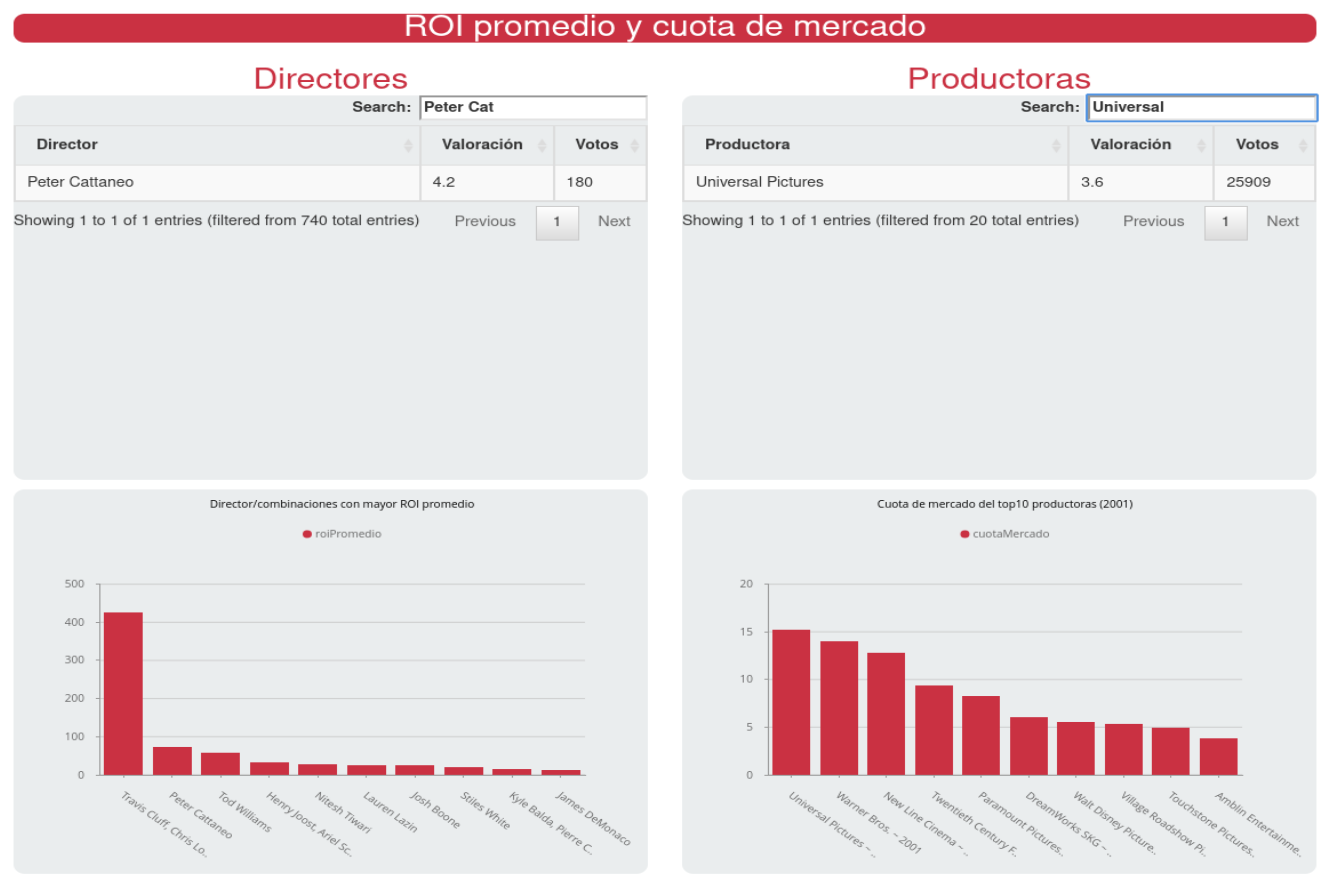
\includegraphics[width=0.5\textwidth]{fotos/1.png}
\caption{Esquema conceptual de un TIS}
\label{fig:1}
\end{figure}

\noindent Existen varias formas de organizar la información en un TIS:

\begin{itemize}
    \item \textbf{Búsqueda}: toma una consulta del usuario y devuelve documentos relevantes.
    \item \textbf{Filtrado y Recomendación}: monitoriza el flujo de datos, selecciona los ítems relevantes para los intereses del usuario y luego recomienda los items relevantes (o filtra los no relevantes). Un sistema de recomendación tiene como objetivo recomendar información relevante al usuario, mientras que un sistema de filtrado tiene como objetivo filtrar la información no relevante, permitiendo que el usuario mantenga solo los \textit{items} relevantes.
    \item \textbf{Categorización}: clasifica un objeto textual en una o varias categorías predefinidas. Puede anotar los objetos con todo tipo de categorías significativas, enriqueciendo la representación de los datos textuales. En este caso hay dos tipos de errores, los falsos positivos y los falsos negativos; hay que ver que métrica de rendimiento se le da al clasificador, dando más o menos \textit{penalty} a un error concreto. Estos sistemas son tradicionales, y se usaban para, por ejemplo, clasificar correos electrónicos como \textit{spam}.
    \item \textbf{Resumen}: toma uno o varios documentos de texto y genera un resumen conciso de los contenidos esenciales. Reduce el esfuerzo humano de digerir grandes cantidades de información textual.
    \item \textbf{Análisis de temáticas}: toma una serie de documentos y extrae y analiza los temas en ellos. Los temas aydan a digerir la información y permiten navegar por el texto de forma cómoda. Se puede combinar con datos no textuales, como tiempo, localización u otros metadatos. De este modo, es capaz de generar patrones de interés (tendencias temporales de temáticas, distribución espacio-temporal del tópicos, etc). Es tecnología no supervisada, por lo que los temas no están predefinidos, los da el propio algoritmo.
    \item \textbf{Extracción de información}: Extrae entidades y relaciones de entidades con otras áreas de conocimiento. 
    \item \textbf{Clustering}: descubre grupos de objetos textuales similares (términos, oraciones, documentos, etc). Ayuda a los usuarios a explorar un espacio de la información, y es útil para descrubrir \textit{outliers}. 
    \item \textbf{Visualización}: permite representar visualmente patrones en los datos textuales.
\end{itemize}
\chapter{Datos textuales}\label{Chapter2} 
% chktex-file 8
% chktex-file 12
% chktex-file 13
% chktex-file 44

\section{Procesamiento de lenguaje natural}

El procesamiento de lenguaje natural (NLP) se ocupa de desarrollar técnicas computacionales para permitir que una computadora entienda el significado del texto en lenguaje natural. El NLP es una base fundamental de los sistemas de información textual (TIS) porque la efectividad de un TIS en ayudar a los usuarios a acceder y analizar datos textuales depende en gran medida de qué tan bien el sistema pueda entender el contenido de los datos textuales. Por lo tanto, el análisis de contenido es lógicamente el primer paso en el análisis y gestión de datos textuales. \\

Mientras que un humano puede entender instantáneamente una oración en su idioma nativo, resulta bastante complicado para un ordenador. En general, esto puede involucrar las siguientes tareas.
\begin{itemize}
\item Análisis léxico: determina las unidades significativas básicas en un idioma, como palabras. Determina el significado de cada palabra y delimita las fronteras de las palabras. Esto último puede ser más complicado en idiomas como el chino.
\item Análisis sintáctico: determinar cómo se relacionan las palabras entre ellas dentro de una oración. Permite obtener más conocimiento que un análisis léxico, pero no tiene por qué tener idea del significado; no hay conocimiento.
\item Análisis semántico: determina el significado de una oración. Esto típicamente implica el cálculo del significado de una oración completa o una unidad mayor basada en los significados de las palabras y su estructura sintáctica. Aquí es cuando se empieza a obtener conocimiento real. 
\item Análisis pragmático: determina el significado en contexto, por ejemplo, inferir los actos de habla del lenguaje. Una comprensión más profunda del lenguaje natural que el análisis semántico es, por lo tanto, entender aún más el propósito en la comunicación.
\item Análisis del discurso: analiza segmentos extensos de texto, considerando varias oraciones, conexiones entre ellas y el contexto en el que se encuentran, considerando el resto de oraciones. Esto es lo que se busca que haga la tecnología (``te lo digo para que hagas algo al respecto''). Este tipo de análisis es muy complicado para textos de lenguaje natural no restringidos, y la tecnología ``pre \textit{deep learning}'' lo hacía muy mal. 
\end{itemize}

\begin{figure}[h]
\centering
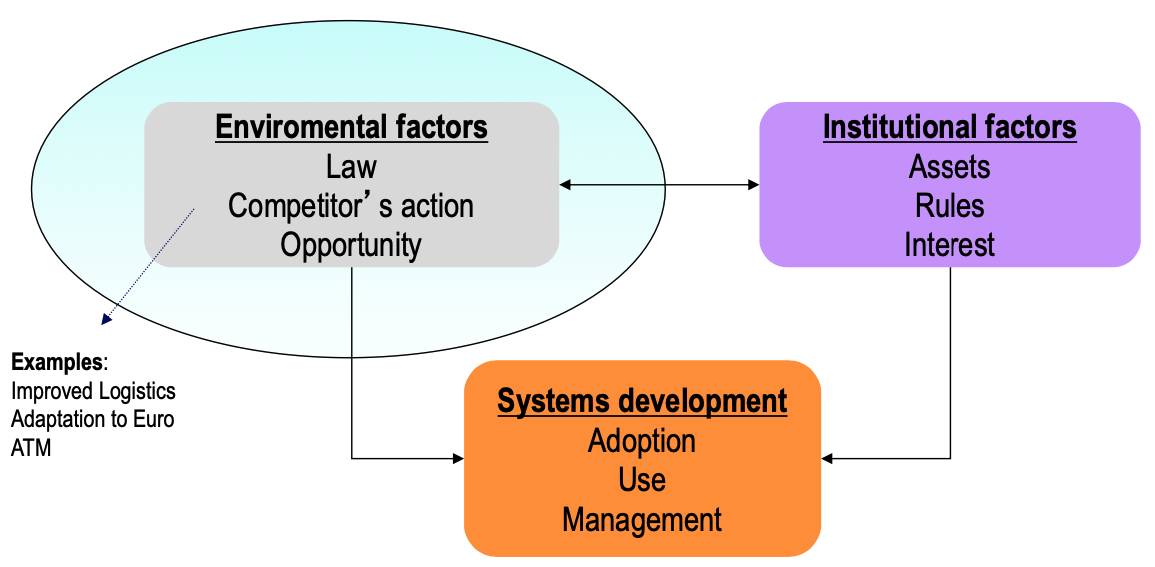
\includegraphics[width=0.7\textwidth]{fotos/2.png}
\caption{Ejemplo de las tareas en el procesamiento de lenguaje natural.}
\label{fig:3.1}
\end{figure}

En la figura \ref{fig:3.1}, se muestra lo que implica entender una oración muy simple en inglés: \textit{A dog is chansing a boy on the playground}. El análisis léxico en este caso implica determinar las categorías sintácticas (partes del discurso) de todas las palabras (por ejemplo, ``\textit{dog}'' es un sustantivo y ``\textit{chasing}'' es un verbo). El análisis sintáctico consiste en determinar que ``\textit{a}'' y ``\textit{boy}'' forman una frase nominal. Lo mismo ocurre con ``\textit{the}'' y ``\textit{playground}'', y ``\textit{on the playground}'' es una frase preposicional. El análisis semántico consiste en mapear las frases nominales a entidades y las frases verbales a relaciones para obtener una representación formal del significado de la oración. Por ejemplo, la frase nominal ``\textit{a boy}'' puede mapearse a una entidad semántica que denota a un niño (es decir, b1), y ``\textit{a dog}'' a una entidad que denota a un perro (es decir, d1). La frase verbal puede mapearse a un predicado de relación ``\textit{chasing}(d1, b1, p1)'' como se muestra en la figura. Nótese que con este nivel de comprensión, también se puede inferir información adicional basada en cualquier conocimiento de sentido común relevante. Por ejemplo, si se asume que si alguien está siendo perseguido puede estar asustado, se podría inferir que el niño que está siendo perseguido (b1) puede estar asustado. Finalmente, el análisis pragmático podría revelar además que la persona que dijo esta oración podría tener la intención de solicitar una acción, como recordar al dueño del perro que vigile al perro. 

\subsection{Desafíos y ambigüedades}

Si bien es posible derivar una representación semántica clara para una oración simple como la que se muestra en la figura \ref{fig:3.1}, en general es muy cimplicado hacer este tipo de análisis para texto en lenguaje natural no restringido. La razón principal de esta dificultad es que el lenguaje natural está diseñado para hacer la comunicación humana eficiente; esto contrasta con un lenguaje de programación, que está diseñado para facilitar la comprensión por parte del ordenador. Específicamente, hay dos razones por las cuales el NLP es muy difícil. 
\begin{itemize}
    \item Se omite mucho conocimiento de sentido común en la comunicación en lenguaje natural porque se asumie que el receptor posee dicho conocimiento (por lo tanto, no hay necesidad de comunicarlo explícitamente).
    \item Se mantienen muchas ambigüedades, que se asumen que el receptor sabe cómo resolver (por lo tanto, no hay necesidad de gastar palabras para aclararlas). Como resultado, el texto en lenguaje natural está lleno de ambigüedad, y resolverla generalmente implicaría razonar con una gran cantidad de conocimiento de sentido común, lo cual es un desafío en inteligencia artificial.
\end{itemize}

En este sentido, el NLP es "completo en IA", es decir, tan difícil como cualquier otro problema complicado en inteligencia artificial.Algunos tipos de ambigüedades a las que hay que enfrentarse en NLP son:
\begin{itemize}
\item Ambigüedad a nivel de palabra: Una palabra puede tener múltiples categorías sintácticas o significados. Por ejemplo, ``diseño'' como sustantivo o verbo, (POS ambiguo) o palabras polisémicas (sentido ambiguo).
\item Ambigüedad sintáctica: Las oraciones pueden tener múltiples estructuras sintácticas. Por ejemplo, procesamiento de lenguaje natural puede tener dos interpretaciones diferentes: ``procesado del lenguaje natural'' o ``procesado natural del lenguaje'' (modificación ambigua). ``Un hombre vio a un niño con un telescopio,'' que tiene interpretaciones diferentes que conducen a significados distintos (adjunción ambigua de frase preposicional (PP)).
\item Resolución de anáforas: Determina a qué se refiere un pronombre, lo cual puede ser poco claro. ``\textit{John persuaded Bill to buy a TB for himself}'', donde ``himself'' puede referirse a John o a Bill.
\item Presuposición: Implica suposiciones, como en ``Él ha dejado de fumar'' implicando que fumaba antes. Hacer este tipo de inferencias resulta generalmente complicado. 
\end{itemize}

\subsection{Historia y estado del arte en NLP}

La investigación en NLP se remonta al menos a la década de 1950, cuando los investigadores eran muy optimistas sobre tener ordenadores capaces de entender el lenguaje humano, particularmente con el propósito de la traducción automática. Sin embargo, pronto quedó claro que la traducción de alta calidad completamente automática no podría lograrse sin conocimiento. Un diccionario resultaba insuficiente; en su lugar, haría falta una enciclopedia. \\

Al darse cuenta de que la traducción automática podría ser demasiado ambiciosa, los investigadores abordaron aplicaciones menos ambiciosas de NLP a finales de la década de 1960 y 1970 con cierto éxito, aunque las técnicas desarrolladas no lograron escalar, teniendo así un impacto limitado en las aplicaciones. Por ejemplo, la gente probó aplicaciones de reconocimiento de voz donde el objetivo es transcribir un discurso. Esta tarea requiere solo una comprensión limitada del lenguaje natural, por lo tanto, es más realista. Se desarrollaron dos proyectos que demostraron la capacidad del ordenador para entender el lenguaje natural: uno es el proyecto Eliza, donde se utilizan reglas superficiales para permitir que un ordenador juegue el papel de un terapeuta para entablar un diálogo en lenguaje natural con un humano; el otro es el proyecto del mundo de bloques, que demostró la viabilidad de la comprensión semántica profunda del lenguaje natural cuando el lenguaje se limita a un dominio de juguete con solo bloques como objetos. \\

En las décadas de 1970 y 1980, se prestó atención al procesamiento de datos textuales en lenguaje natural del mundo real, particularmente a la comprensión de historias. Se desarrollaron muchos formalismos para la representación del conocimiento y reglas heurísticas de inferencia. Sin embargo, la conclusión general fue que incluso las historias simples son bastante difíciles de entender por un ordenador, confirmando la necesidad de una representación del conocimiento a gran escala e inferencias bajo incertidumbre. \\

Después de la década de 1980, los investigadores comenzaron a alejarse de los enfoques simbólicos tradicionales (basados en lógica) para el procesamiento del lenguaje natural, que en su mayoría habían demostrado no ser robustos para aplicaciones reales, y prestaron más atención a los enfoques estadísticos, que dieron más éxito; inicialmente en el reconocimiento de voz, y posteriormente en prácticamente el resto de tareas de NLP. A diferencia de los enfoques simbólicos, los enfoques estadísticos tienden a ser más robustos porque dependen menos de reglas generadas por humanos; en su lugar, a menudo aprovechan las regularidades y patrones en los usos empíricos del lenguaje, y se basan únicamente en datos de entrenamiento etiquetados por humanos y en la aplicación de técnicas de aprendizaje automático. \\

Si bien el conocimiento lingüístico siempre es útil, hoy en día, las técnicas de procesamiento del lenguaje natural más avanzadas tienden a depender en gran medida del uso intensivo de técnicas de aprendizaje automático estadístico, con el conocimiento lingüístico jugando solo un papel secundario. Estas técnicas de NLP estadístico son exitosas para algunas de las tareas de NLP. 

\subsection{Procesamiento de lenguaje natural estadístico}

El NLP estadístico se basa en la probabilidad y en la estadística para resolver problemas de lenguaje natural. Algunas tareas comunes son:
\begin{itemize}
\item El etiquetado de partes del discurso (POS) es una tarea relativamente fácil, y los etiquetadores de POS en el estado del arte pueden tener una precisión muy alta (por encima del 97\% en datos de noticias).
\item El análisis sintáctico (\textit{parsing}) es más difícil, aunque el análisis sintáctico parcial se puede hacer con una precisión razonablemente alta (por ejemplo, por encima del 90\% para el reconocimiento de frases nominales).
\begin{figure}[H]
\centering
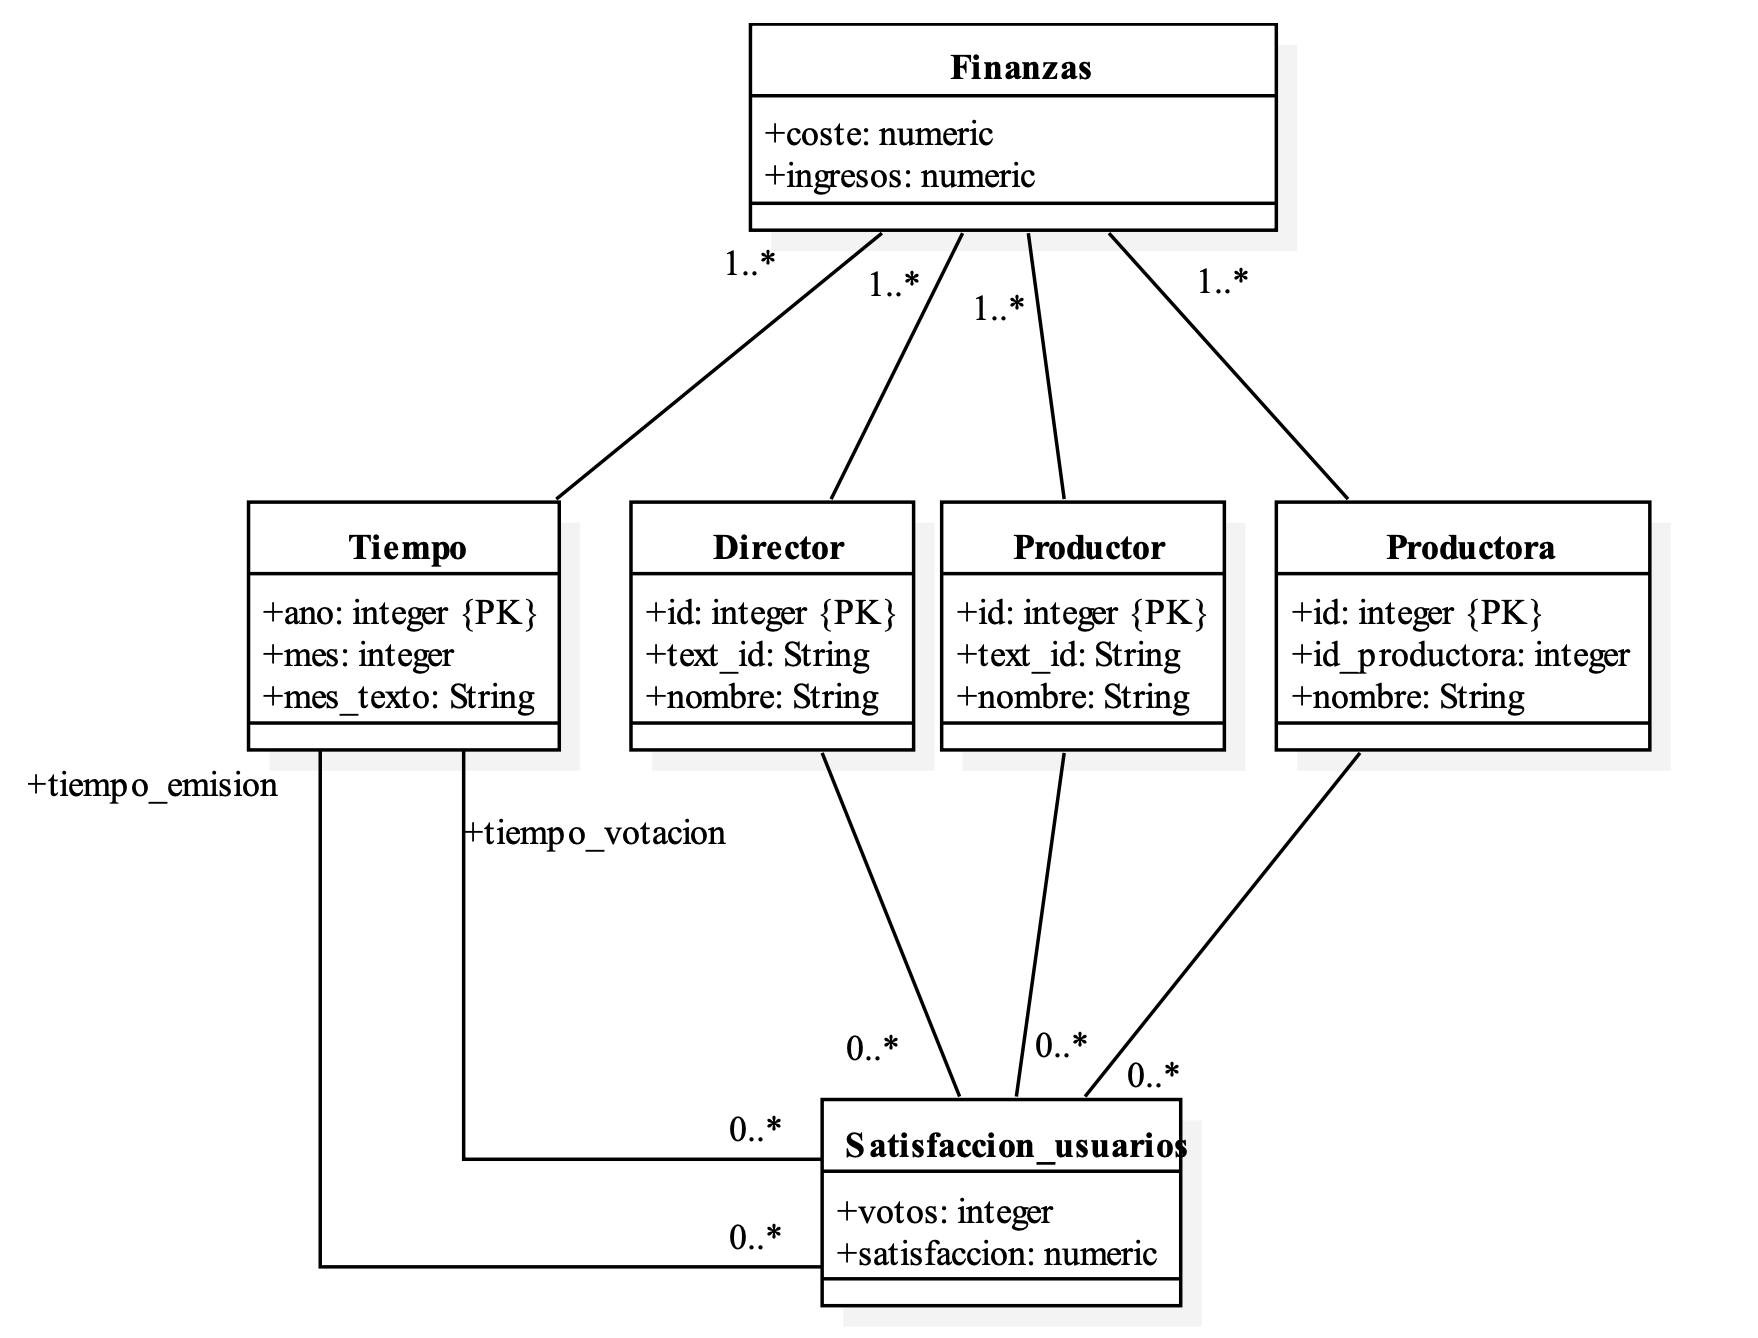
\includegraphics[width=0.25\textwidth]{fotos/3.png}
\caption{Ejemplo de análisis sintáctico.}
\label{fig:3}
\end{figure}
\item Análisis completo de estructura (\textit{full structure parsing}): es una tarea muy complicada debido a las ambigüedades en el lenguaje natural.
\item Análisis semántico: asigna un significado a una oración. Es una tarea aún más complicada, con éxito limitado. Extracción de información notable(se reconocen entidades nombradas como nombres de personas y organizaciones, y relaciones entre entidades como quién trabaja en qué organización), la desambiguación del sentido de las palabras (distinguir diferentes sentidos de una palabra en diferentes contextos de uso) y el análisis de sentimientos (reconocer opiniones positivas sobre un producto en una reseña de producto) son áreas de interés. Inferencias y habla.
\item Análisis de actos: determina la intención detrás de la comunicación. Generalmente, solo es factible en dominios muy limitados.
\end{itemize}

\subsubsection{Procesamiento de lenguaje natural superficial y profundo}   

En textos arbitrarios, solo el análisis superficial del lenguaje natural se puede hacer de forma robusta. El análisis profundo no escala bien, y no es robusto para textos no restringidos. Este último, además, requiere una cantidad significativa de datos de entrenamiento (etiquetados por humanos) para obtener una precisión razonable.

\begin{figure}[h]
\centering
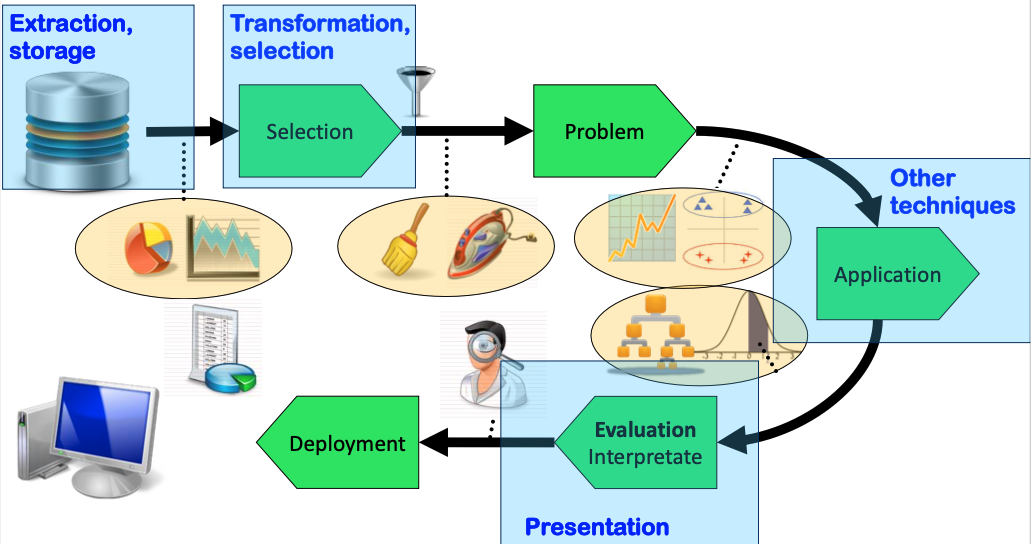
\includegraphics[width=0.5\textwidth]{fotos/4.png}
\caption{Dificultad de varias aplicaciones de NLP.}
\label{fig:4}
\end{figure}

\section{Representación de texto}

Las técnicas de NLP permiten diseñar muchos tipos diferentes de características informativas para los objetos textuales. Como ejemplo, la oración \textit{A dog is chasing a boy on the playground} en la figura \ref{fig:3.3}. Se puede representar esta oración de muchas formas distintas. Primero, siempre se puede representar dicha oración como una cadena de caracteres. Esto es cierto para todos los idiomas, y es quizás la forma más general de representar texto, ya que siempre puede usarse este enfoque para representar cualquier dato textual. Desafortunadamente, la desventaja de esta representación es que no permite realizar análisis semántico, que a menudo es necesario en muchas aplicaciones de minería de texto. No se están reconociendo palabras, que son la unidad básica de significado para cualquier idioma. \\

La siguiente versión de la representación del texto es realizar la segmentación de palabras para obtener una secuencia de palabras. En la oración de ejemplo, se obtienen características como ``\textit{dog}'' y ``\textit{chasing}''. Con este nivel de representación se tiene mucha más libertad. Al identificar palabras, se puede, por ejemplo, descubrir fácilmente las palabras más frecuentes en un documento o en toda la colección. Estas palabras luego se pueden usar para formar temas. Por lo tanto, representar datos textuales como una secuencia de palabras abre muchas posibilidades de análisis interesantes. \\

Sin embargo, este nivel de representación es ligeramente menos general que una cadena de caracteres. En algunos idiomas, como el chino, no es tan fácil identificar todos los límites de las palabras. Para resolver este problema, se confia en algunas técnicas especiales para identificar palabras y realizar una segmentación más avanzada que no se base solo en los espacios en blanco (lo que no siempre es 100\% preciso). Por lo tanto, la representación de la secuencia de palabras no es tan robusta como la representación de la cadena de caracteres. En inglés, es muy fácil obtener este nivel de representación, por lo que puede usarse todo el tiempo. \\

Avanzando más en el procesamiento del lenguaje natural, podemos agregar etiquetas de partes del discurso (POS) a las palabras. Esto permite contar, por ejemplo, los sustantivos más frecuentes, o determinar qué tipo de sustantivos están asociados con qué tipo de verbos. Esto abre más oportunidades para un análisis más profundo. Nótese en la figura \ref{fig:3.3} se usa un signo más en las características adicionales porque al representar el texto como una secuencia de etiquetas de partes del discurso, no necesariamente se reemplaza la secuencia de palabras original. En su lugar, se agrega esto como una forma adicional de representar datos textuales. \\

Representar el texto tanto como palabras como etiquetas de POS enriquece la representación de los datos textuales, permitiendo un análisis más profundo y fundamentado. Si se avanza más, entonces se estaría analizando la oración para obtener una estructura sintáctica. Esto abre más análisis de, por ejemplo, los estilos de escritura o la corrección de errores gramaticales. \\

Avanzando más en el análisis semántico, se podría reconocer ``\textit{dog}'' como un animal. También podemos reconocer ``\textit{boy}'' como una persona, y ``\textit{playground}'' como una ubicación y analizar sus relaciones. Una deducción podría ser que el perro estaba persiguiendo al niño, y el niño está en el parque. Esto agregará más entidades y relaciones, a través del reconocimiento de relaciones entre entidades. Ahora, se puede contar la persona más frecuente que aparece en toda esta colección de artículos de noticias. Estos tipos de patrones repetidos pueden potencialmente dar muy buenas características. \\

Esta representación de alto nivel es aún menos robusta que la secuencia de palabras o las etiquetas de POS, pero es muy útil. No siempre es fácil identificar todas las entidades con los tipos correctos y se pueden cometer errores. Las relaciones son aún más difíciles de encontrar. Si se mueve hacia una representación lógica, entonces existen predicados y reglas de inferencia. Con reglas de inferencia se pueden inferir hechos derivados interesantes del texto. No se puede hacer eso todo el tiempo para todo tipo de oraciones, ya que puede llevar un tiempo de computación significativo o una gran cantidad de datos de entrenamiento. \\

Finalmente, los actos de habla agregarían otro nivel de representación de la intención de esta oración. En este ejemplo, podría ser una solicitud. Saber eso permitiría analizar cosas aún más interesantes sobre el emisor de esta oración. ¿Cuál es la intención de decir eso? ¿Qué escenarios o qué tipos de acciones ocurrirán?

\begin{figure}[h]
\centering
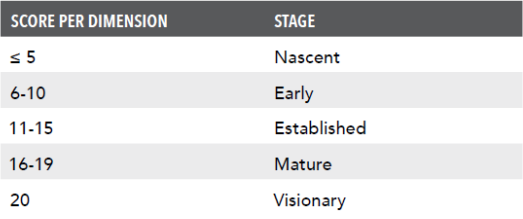
\includegraphics[width=0.7\textwidth]{fotos/5.png}
\caption{Diferentes niveles de representación de texto.}
\label{fig:3.3}
\end{figure}

Las técnicas de NLP más sofisticadas requieren más esfuerzo humano, y generalmente son menos robustas ya que intentan resolver un problema mucho más difícil. Si se analiza el texto en niveles que representan un análisis más profundo del lenguaje, entonces hay que tolerar posibles errores. Eso también significa que aún es necesario combinar dicho análisis profundo con análisis superficial basado en, por ejemplo, secuencias de palabras. A medida que se avanza, la representación del texto está más cerca de la representación del conocimiento en la mente humana; ese es el propósito de la minería de texto. \\

En la representación de textos hay que buscar un balance, un compromiso entre un análisis profundo, que puede dar errores pero dará un conocimiento directo que puede ser extraído del texto, y un análisis superficial, que es robusto pero no aportará una represención del conocimiento con el detalle adecuado. \\

Diferentes representaciones de texto tienden a permitir diferentes análisis, como se muestra en la figura \ref{fig:3.4}. En particular, se agregan gradualmente resultados de análisis más profundos para representar datos textuales que abrirían más oportunidades de representación y capacidades de análisis. 

\begin{figure}[h]
\centering
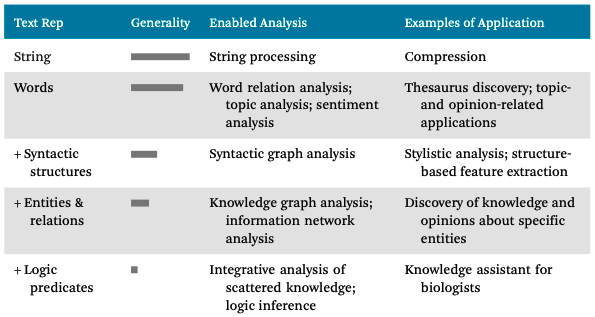
\includegraphics[width=0.7\textwidth]{fotos/8.png}
\caption{Representación de texto y análisis permitido.}
\label{fig:3.4}
\end{figure}

\section{Modelos de lenguaje estadísticos}

Un modelo de lenguaje estadístico proporciona una distribución de probabilidad sobre secuencias de palabras, por ejemplo, 
\begin{align*}
p(\text{\textit{Today is Wednesday}}) &= 0.001 \\
p(\text{\textit{Today Wednesday is}}) &= 0.000000001 \\
p(\text{\textit{The equation has a solution}}) &= 0.000001
\end{align*} 

Un modelo de lenguaje puede depender del contexto. En el modelo de lenguaje mostrado anteriormente, la secuencia ``\textit{The equation has a solution}'' tiene una probabilidad menor que ``\textit{Today is Wednesday}''. Esto puede ser un modelo de lenguaje razonable para describir conversaciones generales, pero puede ser inexacto para describir conversaciones que ocurren en una conferencia de matemáticas, donde la secuencia ``\textit{The equation has a solution}'' puede ocurrir con más frecuencia que ``\textit{Today is Wednesday}''. \\

Sea un modelo de lenguaje, se pueden muestrear secuencias de palabras de acuerdo con la distribución para obtener una muestra de texto. En este sentido, podemos usar dicho modelo para ``generar'' texto. Por lo tanto, un modelo de lenguaje también se denomina a menudo un modelo generativo para texto. 

\subsection{Usos de modelos del lenguaje}

\begin{itemize}
\item Reconocimiento de voz: Predice secuencias probables de palabras. Si se escucha, por ejemplo, \textit{John feels}, se puede predecir que la siguiente palabra será \textit{happy}, aunque haya palabras similares acústicamente, como \textit{habit}. Esto es debido a que una es más probable que la otra. 
\item Categorización de texto: Determina la probabilidad de temas. Por ejemplo, si se tien \textit{baseball} tres vces y \textit{game} una en un artículo, ¿cómo de probable es que el tema sea ``deportes''?
\item Recuperación de información: Mejora la relevancia en búsquedas. Si un usuario está interesado en noticias de deportes, ¿cómo de probable es que se use la palabra \textit{baseball} en una consulta?
\end{itemize}

\subsection{Modelos de lenguaje}

Si se enumeran todas las posibles secuencias de palabras y se asigna una probabilidad a cada secuencia, el modelo sería demasiado complejo de estimar, ya que el número de parámetros es potencialmente infinito al tener un número potencialmente infinito de secuencias de palabras. Es decir, nunca se dispondría de suficientes datos como para estimar estos parámetros. Por lo tanto, se deben hacer suposiciones para simplificar el modelo. \\

El modelo de lenguaje más simple es el modelo de lenguaje unigrama, en el cual se asume que una secuencia de palabras resulta de generar cada palabra de manera independiente. Por lo tanto, la probabilidad de una secuencia de palabras sería igual al producto de la probabilidad de cada palabra. Formalmente, sea $V$ el conjunto de palabras en el vocabulario, y $w_1, \dots, w_n$ una secuencia de palabras, donde $w_i \in V$ es una palabra. Así, la probabilidad de la secuencia de palabras sería
\begin{equation}
p(w_1, \dots, w_n) = \prod_{i=1}^n p(w_i)
\end{equation}

Dado un modelo de lenguaje unigrama $\theta$, habrá tantos parámetros como palabras en el vocabulario, y estos satisfacen la restricción $\sum_{w \in V} p(w) = 1$. Tal modelo esencialmente especifica una distribución multinomial sobre todas las palabras. \\

Dado un modelo de lenguaje $\theta$, en general, las probabilidades de generar dos documentos diferentes $D_1$ y $D_2$ serían diferentes, es decir, $p(D_1 | \theta) \neq p(D_2 | \theta)$. Intuitivamente, los documentos con mayor probabilidad serían aquellos que contienen muchas ocurrencias de las palabras de alta probabilidad según $p(w | \theta)$. En este sentido, las palabras de alta probabilidad de $\theta$ pueden indicar el tema capturado por $\theta$. \\

\begin{figure}[h]
\centering
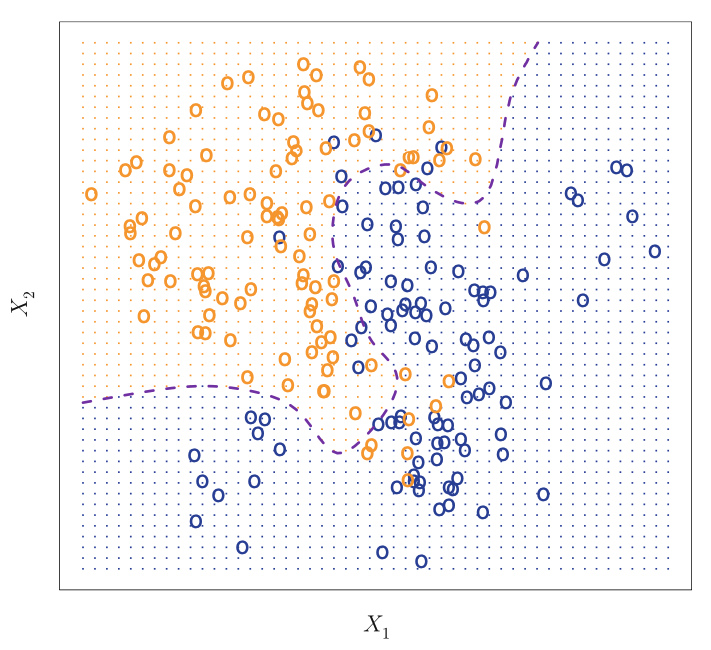
\includegraphics[width=0.4\textwidth]{fotos/9.png}
\caption{Dos ejemplos de modelos de lenguaje unigrama, representando dos temas distintos.}
\label{fig:9}
\end{figure}

Por ejemplo, los dos modelos de lenguaje unigrama ilustrados en la Figura \ref{fig:9} sugieren un tema sobre ``minería de texto'' y un tema sobre ``salud'', respectivamente. Intuitivamente, si $D$ es un artículo sobre minería de texto, se esperaría que $p(D | \theta_1) > p(D | \theta_2)$, mientras que si $D'$ es un artículo de blog que discute el control de la dieta, se esperaría lo contrario: $p(D' | \theta_1) < p(D' | \theta_2)$. También se puede esperar que $p(D | \theta_1) > p(D' | \theta_1)$ y $p(D | \theta_2) < p(D' | \theta_2)$. \\

Sea ahora un documento $D$ que se asume que ha sido generado utilizando un modelo de lenguaje unigrama $\theta$, y se quiere inferir el modelo subyacente $\theta$ (es decir, estimar las probabilidades de cada palabra $w$, $p(w | \theta)$) basado en el documento observado $D$. Este es un problema estándar en estadística llamado estimación de parámetros y puede resolverse utilizando muchos métodos diferentes. \\

Un método popular es el estimador de máxima verosimilitud (ML), que busca un modelo $\hat{\theta}$ que daría a los datos observados la mayor verosimilitud (es decir, que mejor explique los datos):
\begin{equation}
\hat{\theta} = \text{arg max}_{\theta} p(D | \theta)
\end{equation}

Es fácil demostrar que la estimación ML de un modelo de lenguaje unigrama da a cada palabra una probabilidad igual a su frecuencia relativa en $D$. Esto es,
\begin{equation}
p(w | \hat{\theta}) = \frac{\text{c}(w, D)}{|D|}
\end{equation}

donde $c(w, D)$ es el conteo de la palabra $w$ en $D$ y $|D|$ es la longitud de $D$, o el número total de palabras en $D$. \\

Esta estimación es óptima en el sentido de que maximizaría la probabilidad de los datos observados, pero si realmente es adecuada para una aplicación sigue siendo cuestionable. Por ejemplo, si el objetivo es estimar el modelo de lenguaje en la mente de un autor de un artículo de investigación, y usamos el estimador de máxima verosimilitud para estimar el modelo basado solo en el resumen de un artículo, entonces claramente no es correcto, ya que el modelo estimado asignaría una probabilidad cero a cualquier palabra no vista en el resumen, lo que haría que todo el artículo tuviera una probabilidad cero a menos que solo use palabras del resumen. En general, la estimación de máxima verosimilitud asignaría una probabilidad cero a cualquier \textit{token} o evento no observado en los datos; esto es así porque asignar una probabilidad no nula a dicho \textit{token} quitaría masa de probabilidad que podría haberse asignado a una palabra observada (ya que todas las probabilidades deben sumar 1), reduciendo así la verosimilitud de los datos observados. Para mejorar el estimador de máxima verosimilitud se usan técnicas de suavizado. \\

\begin{figure}[h]
\centering
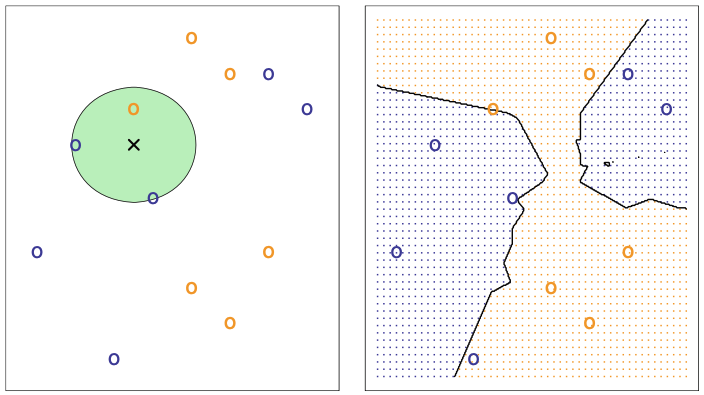
\includegraphics[width=0.7\textwidth]{fotos/10.png}
\caption{Tres modelos de lenguaje diferentes representando tres temas distintos.}
\label{fig:3.6}
\end{figure}

Aunque extremadamente simple, un modelo de lenguaje unigrama es muy útil para el análisis de texto. Por ejemplo, la figura \ref{fig:3.6} muestra tres modelos de lenguaje unigrama diferentes, estimados en tres muestras distintas de datos textuales: una base de datos de texto en inglés general, una base de datos de artículos de investigación en ciencias de la computación y un artículo de investigación sobre minería de texto. En general, las palabras con las probabilidades más altas en los tres modelos son aquellas palabras funcionales en inglés, porque tales palabras se usan frecuentemente en cualquier texto. Bajando más en la lista de palabras, se verían más palabras con contenido y palabras temáticas. Las palabras de contenido serán completamente distintas dependiendo de los datos utilizados para la estimación y, por lo tanto, pueden usarse para discriminar los temas en diferentes muestras de texto. \\

Los modelos de lenguaje unigrama también pueden usarse para realizar análisis semántico de relaciones entre palabras. Por ejemplo, se pueden usarlos para encontrar qué palabras están asociadas semánticamente con una palabra como ``computadora''. La idea principal para hacer esto es ver qué otras palabras tienden a co-ocurrir con esa palabra. Específicamente, primero se puede obtener una muestra de documentos (u oraciones) donde se menciona ``computadora''. Luego se estima un modelo de lenguaje basado en esta muestra para obtener $p(w | \text{computadora})$. Este modelo dice qué palabras ocurren frecuentemente en el contexto de ``computadora''. Sin embargo, las palabras más frecuentes según este modelo probablemente serían palabras funcionales en inglés o palabras que simplemente son comunes en los datos, sin una fuerte asociación con "computadora". Para filtrar las palabras comunes, se necesita un modelo para las mismas, que luego indique qué palabras deben ser filtradas. \\

Es fácil ver que el modelo de lenguaje inglés general (es decir, un modelo de lenguaje de fondo) serviría bien para el propósito. Se puede usar el modelo de lenguaje de fondo para normalizar el modelo $p(w | \text{computadora})$ y obtener una razón, un \textit{ratio} de probabilidad para cada palabra. Las palabras con valores de razón altos pueden entonces asumirse como asociadas semánticamente con ``computadora'', ya que tienden a ocurrir frecuentemente en su contexto, pero no en general. Esto se ilustra en la figura \ref{fig:3.7}.

\begin{figure}[h]
\centering
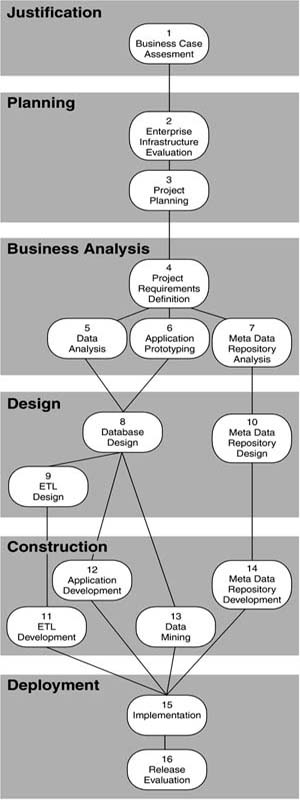
\includegraphics[width=0.7\textwidth]{fotos/11.png}
\caption{Uso de modelos de lenguaje temáticos y modelos de fondo para encontrar palabras semánticamente relacionada.}
\label{fig:3.7}
\end{figure}
\chapter{Clasificacion}\label{Chapter3} 
% chktex-file 8
% chktex-file 12
% chktex-file 13
% chktex-file 44


El modelo de regresión lineal presentado en el capítulo \ref{Chapter3} asume que la variable de respuesta $Y$ es cuantitativa. Sin embargo, en muchas situaciones, la variable de respuesta es cualitativa. A menudo las variables cualitativas se denominan categóricas. Los enfoques para predecir respuestas cualitativas son proceso conocidos como clasificación, ya que implica asignar la observación a una categoría o clase. Por otro lado, frecuentemente los métodos utilizados para clasificación primero predicen la probabilidad de cada una de las categorías de una variable cualitativa, como base para realizar la clasificación. En este sentido, también se comportan como métodos de regresión.

\section{El entorno de clasificación} \label{sec:3.1}

Muchos de los conceptos encontrados en los capítulos anteriores, como el equilibrio entre \textit{bias} y varianza, se transfieren al contexto de clasificación con solo algunas modificaciones debido a que $y_i$ ya no es numérica. Supongamos que se busca estimar $f$ basándose en observaciones de entrenamiento ${(x_1,y_1), \dots,(x_n,y_n)}$, donde ahora $y_1,...,y_n$ son cualitativas. El enfoque más común para cuantificar la precisión de nuestra estimación $\hat{f}$ es la tasa de error de entrenamiento, la proporción de errores que se cometen si se aplica la estimación $\hat{f}$ a las observaciones de entrenamiento:
\begin{equation}
\frac{1}{n}\sum_{i=1}^n I(y_i \neq \hat{y}_i)
\label{eq:2.8}
\end{equation}

Aquí $\hat{y}_i$ es la etiqueta de clase predicha para la $i$-ésima observación usando $\hat{f}$, y $I(y_i \neq \hat{y}_i)$ es una variable indicadora que equivale a 1 si $y_i \neq \hat{y}_i$ y cero si $y_i = \hat{y}_i$. Si $I(y_i \neq \hat{y}_i) = 0$ entonces la $i$-ésima observación fue clasificada correctamente por nuestro método de clasificación; de lo contrario fue mal clasificada. Por lo tanto, la ecuación \ref{eq:2.8} calcula la fracción de clasificaciones incorrectas. \\

La ecuación \ref{eq:2.8} se conoce como la tasa de error de entrenamiento porque se calcula basándose en los datos que se utilizaron para entrenar el clasificador. Como en el contexto de regresión, se está más interesado en las tasas de error que resultan de aplicar nuestro clasificador a observaciones de prueba que no se utilizaron en el entrenamiento. La tasa de error de prueba asociada con un conjunto de observaciones de prueba de la forma $(x_0,y_0)$ está dada por:
\begin{equation}
\text{AVE}(I(y_0 \neq \hat{y}_0))
\label{eq:2.9}
\end{equation}

donde $\hat{y}_0$ es la etiqueta de clase predicha que resulta de aplicar el clasificador a la observación de prueba con predictor $x_0$. Un buen clasificador es aquel para el cual el error de prueba (\ref{eq:2.9}) es mínimo. \\

\subsection{El clasificador de Bayes}

Se puede demostrar que la tasa de error de prueba dada en (\ref{eq:2.9}) se minimiza, en promedio, por un clasificador muy simple que asigna cada observación a la clase más probable, dados sus valores de predictores. En otras palabras, se debe simplemente asignar una observación de prueba con vector de predictores $x_0$ a la clase $j$ para la cual 
\begin{equation}
\Pr(Y = j | X = x_0)
\label{eq:2.10}
\end{equation}

es mayor. Nótese que (\ref{eq:2.10}) es una probabilidad condicional: es la probabilidad de que $Y = j$, dado el vector de predictores observado $x_0$. Este clasificador tan simple se llama clasificador de Bayes. En un problema de dos clases donde solo hay dos posibles valores de respuesta, digamos clase 1 o clase 2, el clasificador de Bayes corresponde a predecir la clase uno si $\text{Pr}(Y = 1 | X = x_0) > 0.5$, y la clase dos en caso contrario. \\

\begin{figure}[h]
\centering
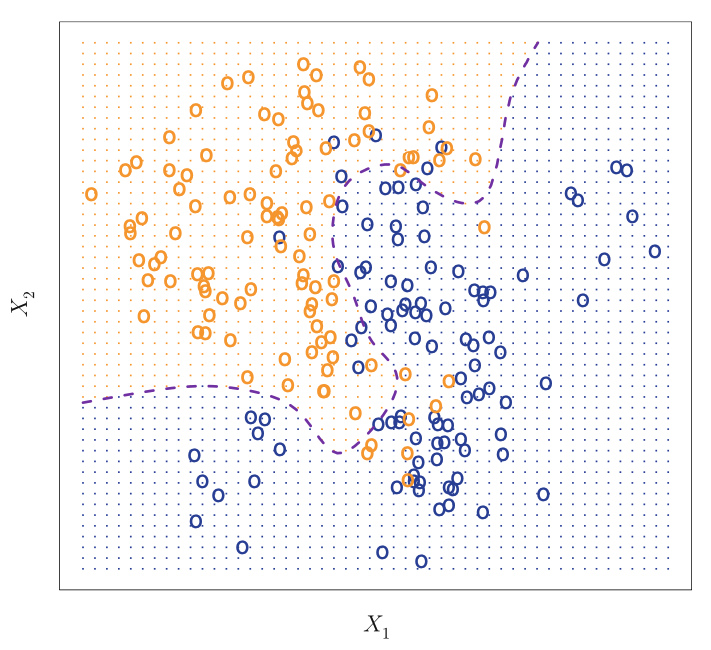
\includegraphics[width=0.6\textwidth]{fotos/9.png}
\caption{Conjunto de datos simulado de 100 observaciones en cada uno de los dos grupos, indicados en azul y en naranja. La línea discontinua púrpura representa la frontera de decisión de Bayes. La cuadrícula de fondo naranja indica la región en la cual una observación de prueba será asignada a la clase naranja, y la cuadrícula de fondo azul indica la región en la cual una observación de prueba será asignada a la clase azul.}
\label{fig:2.13}
\end{figure}

La figura \ref{fig:2.13} proporciona un ejemplo usando un conjunto de datos simulado en un espacio bidimensional que consiste en los predictores $X_1$ y $X_2$. Los círculos naranjas y azules corresponden a observaciones de entrenamiento que pertenecen a dos clases diferentes. Para cada valor de $X_1$ y $X_2$, hay una probabilidad diferente de que la respuesta sea naranja o azul. Dado que estos son datos simulados, se sabe cómo se generaron los datos y se pueden calcular las probabilidades condicionales para cada valor de $X_1$ y $X_2$. La región sombreada en naranja refleja el conjunto de puntos para los cuales $\text{Pr}(Y = \text{naranja} | X)$ es mayor al 50\%, mientras que la región sombreada en azul indica el conjunto de puntos para los cuales la probabilidad es menor al 50\%. La línea discontinua púrpura representa los puntos donde la probabilidad es exactamente del 50\%. Esto se llama la frontera de decisión de Bayes. La predicción del clasificador de Bayes está determinada por la frontera de decisión de Bayes; una observación que cae en el lado naranja de la frontera se asignará a la clase naranja, y de manera similar, una observación en el lado azul de la frontera se asignará a la clase azul. \\

El clasificador de Bayes produce la tasa de error de prueba más baja posible, llamada la tasa de error de Bayes. Dado que el clasificador de Bayes siempre elegirá la clase para la cual (\ref{eq:2.10}) es mayor, la tasa de error en $X = x_0$ será 
\begin{equation}
1 - \max_j \text{Pr}(Y = j | X = x_0)
\end{equation}

\noindent En general, la tasa de error de Bayes global está dada por

\begin{equation}
1 - E\left(\max_j \text{Pr}(Y = j | X)\right)
\end{equation}

donde la expectativa promedia la probabilidad sobre todos los valores posibles de $X$. Para nuestros datos simulados, la tasa de error de Bayes es 0.1304. Es mayor que cero, porque las clases se superponen en la población verdadera, por lo que $\max_j \Pr(Y = j | X = x_0) < 1$ para algunos valores de $x_0$. La tasa de error de Bayes es análoga al error irreducible discutido anteriormente.

\subsection{¿Por qué no regresión lineal?}

Supongamos que se está tratando de predecir la condición médica de un paciente en la sala de emergencias en función de sus síntomas. En este ejemplo simplificado, hay tres posibles diagnósticos: derrame cerebral, sobredosis de drogas y ataque epiléptico. Se podría considerar codificar estos valores como una variable de respuesta cuantitativa, $Y$, de la siguiente manera:
\begin{equation*}
Y = 
\begin{cases} 
0 & \text{si derrame cerebral} \\
1 & \text{si sobredosis de drogas} \\
2 & \text{si ataque epiléptico}
\end{cases}
\end{equation*}

Usando esta codificación, se podría usar mínimos cuadrados para ajustar un modelo de regresión lineal para predecir $Y$ en función de un conjunto de predictores $X_1,...,X_p$. Desafortunadamente, esta codificación implica un orden en los resultados, colocando sobredosis de drogas entre derrame cerebral y ataque epiléptico, e insistiendo en que la diferencia entre derrame cerebral y sobredosis de drogas es la misma que la diferencia entre sobredosis de drogas y ataque epiléptico. En la práctica, no hay ninguna razón particular para que esto sea así. Por ejemplo, se podría elegir una codificación igualmente razonable,
\begin{equation*}
Y = 
\begin{cases} 
0 & \text{si sobredosis de drogas} \\
1 & \text{si derrame cerebral} \\
2 & \text{si ataque epiléptico}
\end{cases}
\end{equation*}

lo que implicaría una relación totalmente diferente entre las tres condiciones. Cada una de estas codificaciones produciría modelos lineales fundamentalmente diferentes que llevarían a diferentes conjuntos de predicciones en observaciones de prueba. \\

Si los valores de la variable de respuesta tuvieran un orden natural, como leve, moderado y severo, y se sintiera que la brecha entre leve y moderado es similar a la brecha entre moderado y severo, entonces una codificación 1, 2, 3 sería razonable. Desafortunadamente, en general no hay una manera natural de convertir una variable de respuesta cualitativa con más de dos niveles en una respuesta cuantitativa que esté lista para la regresión lineal. \\

Para una respuesta cualitativa binaria (de dos niveles), la situación es mejor. Por ejemplo, tal vez solo hay dos posibilidades para la condición médica del paciente: derrame cerebral y sobredosis de drogas. Entonces se podría potencialmente usar el enfoque de variable ficticia para codificar la respuesta de la siguiente manera:
\begin{equation*}
Y = 
\begin{cases} 
0 & \text{si derrame cerebral} \\
1 & \text{si sobredosis de drogas}
\end{cases}
\end{equation*}

Se podría ajustar una regresión lineal a esta respuesta binaria, y predecir sobredosis de drogas si $\hat{Y} > 0.5$ y derrame cerebral en caso contrario. En el caso binario, no es difícil mostrar que incluso si se invierte la codificación anterior, la regresión lineal producirá las mismas predicciones finales. \\

\begin{figure}[h]
\centering
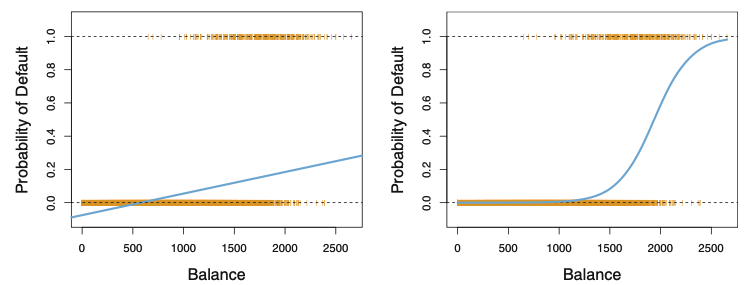
\includegraphics[width=0.6\textwidth]{fotos/14.png}
\caption{Clasificación usando los datos de Default. Izquierda: Probabilidad estimada de incumplimiento usando regresión lineal. ¡Algunas probabilidades estimadas son negativas! Las marcas naranjas indican los valores 0/1 codificados para incumplimiento (No o Sí). Derecha: Probabilidades predichas de incumplimiento usando regresión logística. Todas las probabilidades están entre 0 y 1.}
\label{fig:4.2}
\end{figure}

Para una respuesta binaria con una codificación 0/1 como la anterior, la regresión por mínimos cuadrados tiene sentido; se puede mostrar que el $\hat{X}\beta$ obtenido usando regresión lineal es de hecho una estimación de $\text{Pr}(\text{sobredosis de drogas} | X)$ en este caso especial. Sin embargo, si se usa regresión lineal, algunas de nuestras estimaciones podrían estar fuera del intervalo [0,1] (ver figura \ref{fig:4.2}), lo que las hace difíciles de interpretar como probabilidades. No obstante, las predicciones proporcionan un orden y pueden interpretarse como estimaciones de probabilidad crudas. Curiosamente, resulta que las clasificaciones que se obtienen si se usa regresión lineal para predecir una respuesta binaria serán las mismas que para el procedimiento de análisis discriminante lineal (LDA). \\

Sin embargo, el enfoque de variable ficticia no se puede extender fácilmente para acomodar respuestas cualitativas con más de dos niveles. Por estas razones, es preferible usar un método de clasificación que esté verdaderamente adaptado para valores de respuesta cualitativos, como los que se presentan a continuación.

\section{Regresión logística}

\subsection{Modelo logístico}

Veamos cómo se debe modelar la relación entre $p(X) = \Pr(Y = 1|X)$ y $X$ (por conveniencia se usará la codificación genérica 0/1 para la respuesta). Anteriormentese se habló de usar un modelo de regresión lineal para representar estas probabilidades:
\begin{equation}
p(X) = \beta_0 + \beta_1 X
\label{eq:4.1}
\end{equation}

Si se usa este enfoque para predecir default=Sí usando balance, entonces se obtiene el modelo mostrado en el panel izquierdo de la figura \ref{fig:4.2}. Cada vez que se ajusta una línea recta a una respuesta binaria que está codificada como 0 o 1, en principio siempre se puede predecir $p(X) < 0$ para algunos valores de $X$ y $p(X) > 1$ para otros (a menos que el rango de $X$ esté limitado). \\

Para evitar este problema, se debe modelar $p(X)$ usando una función que dé salidas entre 0 y 1 para todos los valores de $X$. Nótese que la frontera de decisión entre ambas salidas viene dada por $P(Y = 1 |X) = P(Y = 0 | X)$. Muchas funciones cumplen con esta descripción. En la regresión logística, se usa la función logística,
\begin{equation}
p(X) = \frac{e^{\beta_0 + \beta_1 X}}{1 + e^{\beta_0 + \beta_1 X}} = \frac{1}{1 + e^{-(\beta_0 + \beta_1 X)}}
\label{eq:4.2}
\end{equation}

Para ajustar el modelo (\ref{eq:4.2}), se usa un método llamado máxima verosimilitud, que se discute en la siguiente sección. El panel derecho de la figura \ref{fig:4.2} ilustra el ajuste del modelo de regresión logística a los datos de Default. Nótese que para balances bajos ahora se predice la probabilidad de incumplimiento como cercana a cero, pero nunca por debajo. Del mismo modo, para balances altos se predice una probabilidad de incumplimiento cercana a uno, pero nunca por encima. Después de manipular un poco (\ref{eq:4.2}), se encuentra que
\begin{equation}
\frac{p(X)}{1 - p(X)} = e^{\beta_0 + \beta_1 X}
\label{eq:4.3}
\end{equation}

La cantidad $\frac{p(X)}{1 - p(X)}$ se llama las probabilidades (\textit{odds}), y puede tomar cualquier valor entre 0 e $\infty$. Valores de las probabilidades cercanos a 0 e $\infty$ indican probabilidades muy bajas y muy altas de incumplimiento, respectivamente. Al tomar el logaritmo de ambos lados de (\ref{eq:4.3}), se llega a
\begin{equation}
\log\left(\frac{p(X)}{1 - p(X)}\right) = \beta_0 + \beta_1 X
\label{eq:4.4}
\end{equation}

La transformación monótona del lado izquierdo se llama el logaritmo de las probabilidades (\textit{log-odds}) o \textit{logit}. Se ve que el modelo de regresión logística (\ref{eq:4.2}) tiene un \textit{logit} que es lineal en $X$. \\

En un modelo de regresión lineal, $\beta_1$ da el cambio promedio en $Y$ asociado con un aumento de una unidad en $X$. En contraste, en un modelo de regresión logística, aumentar $X$ en una unidad cambia el logaritmo de las probabilidades en $\beta_1$ (\ref{eq:4.4}) o, equivalentemente, multiplica las probabilidades por $e^{\beta_1}$ (\ref{eq:4.3}). Sin embargo, debido a que la relación entre $p(X)$ y $X$ en (\ref{eq:4.2})) no es una línea recta, $\beta_1$ no corresponde al cambio en $p(X)$ asociado con un aumento de una unidad en $X$. La cantidad que $p(X)$ cambia debido a un cambio de una unidad en $X$ dependerá del valor actual de $X$. Pero independientemente del valor de $X$, si $\beta_1$ es positivo, entonces aumentar $X$ estará asociado con un aumento en $p(X)$, y si $\beta_1$ es negativo, entonces aumentar $X$ estará asociado con una disminución en $p(X)$.

\subsection{Estimación de los coeficientes}

Los coeficientes $\beta_0$ y $\beta_1$ en (\ref{eq:4.2}) son desconocidos y deben ser estimados basándose en los datos de entrenamiento disponibles. Aunque se podría usar mínimos cuadrados (no lineales) para ajustar el modelo (\ref{eq:4.4}), el método de máxima verosimilitud es preferible, ya que tiene mejores propiedades estadísticas. La intuición básica detrás del uso de máxima verosimilitud para ajustar un modelo de regresión logística es la siguiente: se intenta encontrar $\hat{\beta}_0$ y $\hat{\beta}_1$ de manera que al insertar estas estimaciones en el modelo para $p(X)$, dado en (\ref{eq:4.2}), se obtenga un número cercano a uno para todos los individuos que cumplieron, y un número cercano a cero para todos los individuos que incumplieron. Esta intuición se puede formalizar usando una ecuación matemática llamada función de verosimilitud:
\begin{equation}
\ell(\beta_0, \beta_1) = \prod_{i:y_i=1}^n p(x_i) \prod_{i':y_{i'} = 0} (1 - p(x_{i'}))
\label{eq:4.5}
\end{equation}

Las estimaciones $\hat{\beta}_0$ y $\hat{\beta}_1$ se eligen para maximizar esta función de verosimilitud. En el contexto de la regresión lineal, el enfoque de mínimos cuadrados es de hecho un caso especial de máxima verosimilitud. \\

Muchos aspectos de la salida de la regresión logística son similares a la salida de la regresión lineal. Por ejemplo, se puede medir la precisión de las estimaciones de los coeficientes calculando sus errores estándar. El estadístico $z$ juega el mismo papel que el estadístico $t$ en la salida de la regresión lineal. Por ejemplo, el estadístico $z$ asociado con $\hat{\beta}_1$ es igual a $\hat{\beta}_1 / SE(\hat{\beta}_1)$, por lo que un valor grande (absoluto) del estadístico $z$ indica evidencia en contra de la hipótesis nula $H_0: \beta_1 = 0$. Esta hipótesis nula implica que $p(X) = \frac{e^{\beta_0}}{1 + e^{\beta_0}}$, en otras palabras, que la probabilidad de incumplimiento no depende del balance. Si el valor $p$ asociado con balance es muy pequeño, se puede rechazar $H_0$. En otras palabras, se concluye que efectivamente hay una asociación entre balance y probabilidad de incumplimiento. \\

Una vez estimados los coeficientes, se pueden hacer predicciones de la probabilidad $\hat{p}(X)$ de forma sencilla 
\begin{equation}
\hat{p}(X) = \frac{1}{1 + e^{-(\hat{\beta}_0 + \hat{\beta}_1 X)}}
\label{eq:4.5.1}
\end{equation}

\subsection{Regresión logística múltiple}

Sea el problea de predecir una respuesta binaria usando múltiples predictores. La regresión logística anterior se puede generalizar de forma inmediata, de modo que el logarímto de las probabilidades serán
\begin{equation}
\log\left(\frac{p(X)}{1 - p(X)}\right) = \beta_0 + \beta_1 X_1 + \beta_2 X_2 + \dots + \beta_p X_p
\label{eq:4.6}
\end{equation}

\noindent y la probabilidad será 
\begin{equation}
p(X) = \frac{1}{1 + e^{-(\beta_0 + \beta_1 X_1 + \beta_2 X_2 + \dots + \beta_p X_p)}}
\label{eq:4.7}
\end{equation}

\subsection{Regresión logística no binaria}

Los modelos de regresión logística de binarios discutidos en las secciones anteriores tienen generalizaciones para múltiples clases, pero en la práctica no se utilizan con tanta frecuencia. Una de las razones es que el método que se discute en la próxima sección, el análisis discriminante, es popular para la clasificación de múltiples clases. 

\section{Análisis discriminante lineal}

La regresión logística implica modelar directamente $\Pr(Y = k | X = x)$ usando la función logística, dada por (\ref{eq:4.7}) para el caso de dos clases de respuesta. Se modela la distribución condicional de la respuesta $Y$, dado el(los) predictor(es) $X$. Ahora se considera un enfoque alternativo y menos directo para estimar estas probabilidades. En este enfoque alternativo (modelo generativo), se modela la distribución de los predictores $X$ por separado en cada una de las clases de respuesta (es decir, dado $Y$), y luego se usa el teorema de Bayes para convertir estas distribuciones en estimaciones de $\text{Pr}(Y = k | X = x)$. Cuando se asume que estas distribuciones son normales, resulta que el modelo es muy similar en forma a la regresión logística. Hay varias razones para usar un método distinto a la regresión logística (modelo discriminante):
\begin{itemize}
\item Cuando las clases están bien separadas, las estimaciones de los parámetros para el modelo de regresión logística son sorprendentemente inestables. El análisis discriminante lineal no sufre de este problema.
\item Si $n$ es pequeño y la distribución de los predictores $X$ es aproximadamente normal en cada una de las clases, el modelo de análisis discriminante lineal es nuevamente más estable que el modelo de regresión logística.
\item El análisis discriminante lineal es popular cuando se tienen más de dos clases de respuesta.
\end{itemize}

\subsection{Teorema de Bayes para clasificación}

\subsubsection{Regla de Bayes}

Sean dos eventos cualesquiera $A$ y $B$. La regla de Bayes establece que para encontrar $P(B | A)$ (probabilidad de que ocurra $B$ dado que $A$ ocurrió), se puede usar la siguiente relación:
\begin{equation}
P(B | A) = \frac{P (A \cap B)}{P(A)} = \frac{P(A | B)P(B)}{P(A)} 
\label{eq:4.8}
\end{equation}

\subsubsection{Regla de Bayes en problemas de clasificación}

Supongamos que se desea clasificar una observación en una de $K$ clases distintas, donde $K \geq 2$, es decir, la variable de respuesta cualitativa $Y$ puede tomar $K$ valores distintos y no ordenados. Sea $\pi_k$ la probabilidad general o \textit{a priori} de que una observación elegida al azar provenga de la $k$-ésima clase; esta es la probabilidad de que una observación dada esté asociada con la $k$-ésima categoría de la variable de respuesta $Y$. Sea $f_k(X) \equiv \text{Pr}(X = x | Y = k)$ la función de densidad de $X$ para una observación que proviene de la $k$-ésima clase. Así, $f_k(x)$ es relativamente grande si hay una alta probabilidad de que una observación en la $k$-ésima clase tenga $X \approx x$, y es pequeña si es muy improbable que una observación en la $k$-ésima clase tenga $X \approx x$. Entonces, el teorema de Bayes establece que
\begin{equation}
\Pr(Y = k | X = x) = \frac{P(X = x | Y = k) P (Y = k)}{P(X = x)} = \frac{\pi_k f_k(x)}{\sum_{l=1}^K \pi_l f_l(x)}
\label{eq:4.10}
\end{equation}

Se usará la abreviatura $p_k(X) = \Pr(Y = k | X = x)$. Esto sugiere que en lugar de calcular directamente $p_k(X)$, simplemente se pueden insertar estimaciones de $\pi_k$ y $f_k(X)$ en (\ref{eq:4.10}). En general, estimar $\pi_k$ es fácil si se tiene una muestra aleatoria de $Y$s de la población: simplemente se calcula la fracción de las observaciones de entrenamiento que pertenecen a la $k$-ésima clase. Sin embargo, estimar $f_k(X)$ tiende a ser más complicado, a menos que se asuman algunas formas simples para estas densidades. Se refiere a $p_k(x)$ como la probabilidad posterior de que una observación $X = x$ pertenezca a la $k$-ésima clase. Es decir, es la probabilidad de que la observación pertenezca a la $k$-ésima clase, dado el valor del predictor para esa observación. \\

Se sabe que el clasificador de Bayes, que clasifica una observación a la clase para la cual $p_k(X)$ es mayor, tiene la tasa de error más baja posible entre todos los clasificadores. (Esto, por supuesto, solo es cierto si los términos en (\ref{eq:4.10}) están todos especificados correctamente). Por lo tanto, si se puede encontrar una manera de estimar $f_k(X)$, entonces se puede desarrollar un clasificador que aproxime al clasificador de Bayes. Esto se verá en las próximas secciones.

\subsection{Análisis discriminante lineal para $p = 1$}

Por ahora, supongamos que $p = 1$, es decir, solo se tiene un predictor. Se desea obtener una estimación para $f_k(x)$ que se pueda insertar en (\ref{eq:4.10}) para estimar $p_k(x)$. Luego se clasificará una observación en la clase para la cual $p_k(x)$ sea mayor. Para estimar $f_k(x)$, primero se harán algunas suposiciones sobre su forma. \\

Supongamos que $f_k(x)$ es normal o gaussiana. En el entorno unidimensional, la densidad normal toma la forma
\begin{equation}
f_k(x) = \frac{1}{\sqrt{2\pi\sigma^2_k}} \exp\left(-\frac{(x - \mu_k)^2}{2\sigma^2_k}\right)
\label{eq:4.11}
\end{equation}

donde $\mu_k$ y $\sigma^2_k$ son los parámetros de media y varianza para la $k$-ésima clase. Por ahora, supongamos además que $\sigma^2_1 = \ldots = \sigma^2_K$, es decir, hay un término de varianza compartido entre todas las $K$ clases, que por simplicidad se puede denotar como $\sigma^2$. Insertando (\ref{eq:4.11}) en (\ref{eq:4.10}), se encuentra que
\begin{equation}
p_k(x) = \frac{\pi_k \frac{1}{\sqrt{2\pi\sigma^2}} \exp\left(-\frac{(x - \mu_k)^2}{2\sigma^2}\right)}{\sum_{l=1}^K \pi_l \frac{1}{\sqrt{2\pi\sigma^2}} \exp\left(-\frac{(x - \mu_l)^2}{2\sigma^2}\right)}
\label{eq:4.12}
\end{equation}

Nótese que en (\ref{eq:4.12}), $\pi_k$ denota la probabilidad a priori de que una observación pertenezca a la $k$-ésima clase. El clasificador de Bayes implica asignar una observación $X = x$ a la clase para la cual (\ref{eq:4.12}) es mayor. Tomando el logaritmo de (\ref{eq:4.12}) y reorganizando los términos, no es difícil mostrar que esto es equivalente a asignar la observación a la clase para la cual
\begin{equation}
\delta_k(x) = x \frac{\mu_k}{\sigma^2} - \frac{\mu_k^2}{2\sigma^2} + \log(\pi_k)
\label{eq:4.13}
\end{equation}

es mayor. Por ejemplo, si $K = 2$ y $\pi_1 = \pi_2$, entonces el clasificador de Bayes asigna una observación a la clase 1 si $2x(\mu_1 - \mu_2) > \mu_2^2 - \mu_1^2$, y a la clase 2 en caso contrario. En este caso, la frontera de decisión de Bayes corresponde al punto donde
\begin{equation}
x = \frac{\mu_1^2 - \mu_2^2}{2(\mu_1 - \mu_2)} = \frac{\mu_1 + \mu_2}{2}
\label{eq:4.14}
\end{equation}

\begin{figure}[h]
\centering
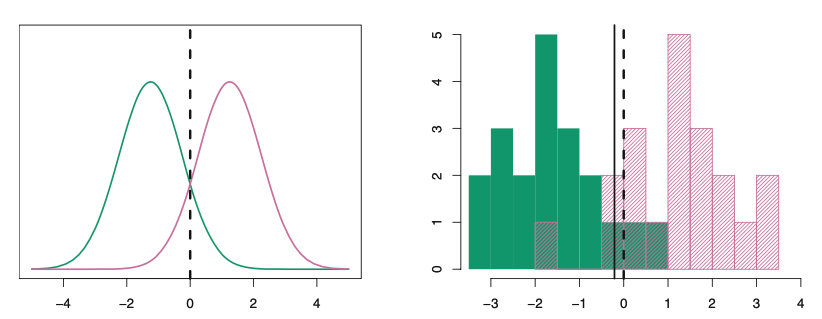
\includegraphics[width=0.7\textwidth]{fotos/15.png}
\caption{Izquierda: Se muestran dos funciones de densidad normal unidimensionales. La línea vertical discontinua representa la frontera de decisión de Bayes. Derecha: Se extrajeron 20 observaciones de cada una de las dos clases, y se muestran como histogramas. La frontera de decisión de Bayes se muestra nuevamente como una línea vertical discontinua. La línea vertical sólida representa la frontera de decisión LDA estimada a partir de los datos de entrenamiento.}
\label{fig:4.4}
\end{figure}

Un ejemplo se muestra en el panel izquierdo de la figura \ref{fig:4.4}. Las dos funciones de densidad normal que se muestran, $f_1(x)$ y $f_2(x)$, representan dos clases distintas. Los parámetros de media y varianza para las dos funciones de densidad son $\mu_1 = -1.25$, $\mu_2 = 1.25$, y $\sigma^2_1 = \sigma^2_2 = 1$. Las dos densidades se superponen, por lo que dado que $X = x$, hay cierta incertidumbre sobre la clase a la que pertenece la observación. Si se asume que una observación es igualmente probable que provenga de cualquiera de las dos clases, es decir, $\pi_1 = \pi_2 = 0.5$, entonces al inspeccionar (\ref{eq:4.14}), se ve que el clasificador de Bayes asigna la observación a la clase 1 si $x < 0$ y a la clase 2 en caso contrario. \\

Nótese que en este caso, se puede calcular el clasificador de Bayes porque se sabe que $X$ se extrae de una distribución gaussiana dentro de cada clase, y se conocen todos los parámetros involucrados. En una situación de la vida real, no se puede calcular el clasificador de Bayes. En la práctica, incluso si se está bastante seguro de la suposición de que $X$ se extrae de una distribución gaussiana dentro de cada clase, aún se deben estimar los parámetros $\mu_1, \ldots, \mu_K$, $\pi_1, \ldots, \pi_K$, y $\sigma^2$. El método de análisis discriminante lineal (LDA) aproxima el clasificador de Bayes insertando estimaciones para $\pi_k$, $\mu_k$, y $\sigma^2$ en (\ref{eq:4.13}). En particular, se usan las siguientes estimaciones:
\begin{equation}
\hat{\mu}_k = \frac{1}{n_k} \sum_{i: y_i = k} x_i, \quad \hat{\sigma}^2 = \frac{1}{n - K} \sum_{k=1}^K \sum_{i: y_i = k} (x_i - \hat{\mu}_k)^2
\label{eq:4.15}
\end{equation}

donde $n$ es el número total de observaciones de entrenamiento, y $n_k$ es el número de observaciones de entrenamiento en la $k$-ésima clase. La estimación para $\mu_k$ es simplemente el promedio de todas las observaciones de entrenamiento de la $k$-ésima clase, mientras que $\hat{\sigma}^2$ se puede ver como un promedio ponderado de las varianzas muestrales para cada una de las $K$ clases. A veces se tiene conocimiento de las probabilidades de pertenencia a la clase $\pi_1, \ldots, \pi_K$, que se pueden usar directamente. En ausencia de cualquier información adicional, LDA estima $\pi_k$ usando la proporción de las observaciones de entrenamiento que pertenecen a la $k$-ésima clase. En otras palabras,
\begin{equation}
\hat{\pi}_k = \frac{n_k}{n}
\label{eq:4.16}
\end{equation}

El clasificador LDA inserta las estimaciones dadas en (\ref{eq:4.15}) y (\ref{eq:4.16}) en (\ref{eq:4.13}), y asigna una observación $X = x$ a la clase para la cual
\begin{equation}
\hat{\delta}_k(x) = x \frac{\hat{\mu}_k}{\hat{\sigma}^2} - \frac{\hat{\mu}_k^2}{2\hat{\sigma}^2} + \log(\hat{\pi}_k)
\label{eq:4.17}
\end{equation}

es mayor. La palabra ``lineal'' en el nombre del clasificador proviene del hecho de que las funciones discriminantes $\hat{\delta}_k(x)$ en (\ref{eq:4.17}) son funciones lineales de $x$ (en lugar de una función más compleja de $x$). \\

El panel derecho de la figura \ref{fig:4.4} muestra un histograma de una muestra aleatoria de 20 observaciones de cada clase. Para implementar LDA, se comenzó estimando $\pi_k$, $\mu_k$, y $\sigma^2$ usando (\ref{eq:4.15}) y (\ref{eq:4.16}). Luego se calculó la frontera de decisión, mostrada como una línea sólida negra, que resulta de asignar una observación a la clase para la cual (\ref{eq:4.17}) es mayor. Todos los puntos a la izquierda de esta línea se asignarán a la clase verde, mientras que los puntos a la derecha de esta línea se asignarán a la clase púrpura. En este caso, dado que $n_1 = n_2 = 20$, se tiene $\hat{\pi}_1 = \hat{\pi}_2$. Como resultado, la frontera de decisión corresponde al punto medio entre las medias muestrales para las dos clases, $(\hat{\mu}_1 + \hat{\mu}_2)/2$. La figura indica que la frontera de decisión LDA está ligeramente a la izquierda de la frontera de decisión óptima de Bayes, que en cambio es igual a $(\mu_1 + \mu_2)/2 = 0$. Dado que estos son datos simulados, se puede generar un gran número de observaciones de prueba para calcular la tasa de error de Bayes y la tasa de error de prueba de LDA. Estas son 10.6\% y 11.1\%, respectivamente. En otras palabras, la tasa de error del clasificador LDA es solo 0.5\% por encima de la tasa de error más baja posible. Esto indica que LDA está funcionando bastante bien en este conjunto de datos. \\

En resumen, el clasificador LDA resulta de suponer que las observaciones dentro de cada clase provienen de una distribución normal con un vector de media específico de la clase y una varianza común $\sigma^2$, e insertar estimaciones para estos parámetros en el clasificador de Bayes. Más adelante, se considerará un conjunto de suposiciones menos estrictas, permitiendo que las observaciones en la $k$-ésima clase tengan una varianza específica de la clase, $\sigma^2_k$.

\subsubsection{Análisis discriminante lineal para $p > 1$}

Para extender el clasificador LDA al caso de múltiples predictores, se asume que $X = (X_1, X_2, \ldots, X_p)$ se extrae de una distribución gaussiana multivariante (o normal multivariante), con un vector de media específico de la clase y una matriz de covarianza común. \\

\begin{figure}[h]
\centering
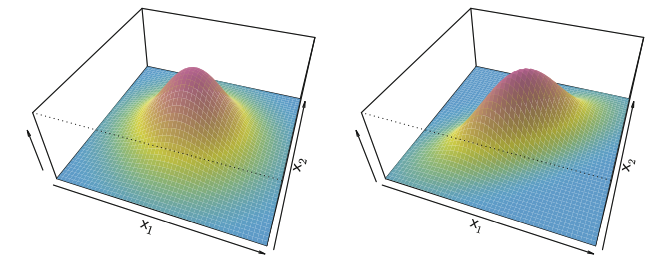
\includegraphics[width=0.7\textwidth]{fotos/16.png}
\caption{}
\label{fig:4.5}
\end{figure}

La distribución gaussiana multivariante asume que cada predictor individual sigue una distribución normal unidimensional, como en (\ref{eq:4.11}), con alguna correlación entre cada par de predictores. Dos ejemplos de distribuciones gaussianas multivariantes con $p = 2$ se muestran en la figura \ref{fig:4.5}. La altura de la superficie en cualquier punto particular representa la probabilidad de que tanto $X_1$ como $X_2$ caigan en una pequeña región alrededor de ese punto. La forma de campana se distorsionará si los predictores están correlacionados o tienen varianzas desiguales, como se ilustra en el panel derecho de la figura \ref{fig:4.5}. En esta situación, la base de la campana tendrá una forma elíptica, en lugar de circular. Para indicar que una variable aleatoria $p$-dimensional $X$ tiene una distribución gaussiana multivariante, escribimos $X \sim N(\mu, \Sigma)$. Aquí $E(X) = \mu$ es la media de $X$ (un vector con $p$ componentes), y $\text{Cov}(X) = \Sigma$ es la matriz de covarianza $p \times p$ de $X$. Formalmente, la densidad gaussiana multivariante se define como
\begin{equation}
f(x) = \frac{1}{(2\pi)^{p/2} |\Sigma|^{1/2}} \exp\left(-\frac{1}{2}(x - \mu)^T \Sigma^{-1} (x - \mu)\right)
\label{eq:4.18}
\end{equation}

En el caso de más de un predictor ($p > 1$), el clasificador LDA asume que las observaciones en la $k$-ésima clase se extraen de una distribución gaussiana multivariante $N(\mu_k, \Sigma)$, donde $\mu_k$ es un vector de media específico de la clase, y $\Sigma$ es una matriz de covarianza común a todas las $K$ clases. Insertando la función de densidad para la $k$-ésima clase, $f_k(X = x)$, en (\ref{eq:4.10}) y realizando un poco de álgebra, se revela que el clasificador de Bayes asigna una observación $X = x$ a la clase para la cual
\begin{equation}
\delta_k(x) = x^T \Sigma^{-1} \mu_k - \frac{1}{2} \mu_k^T \Sigma^{-1} \mu_k + \log(\pi_k)
\label{eq:4.19}
\end{equation}

\noindent es mayor. Esta es la versión vector/matriz de (\ref{eq:4.13}). \\

\begin{figure}[h]
\centering
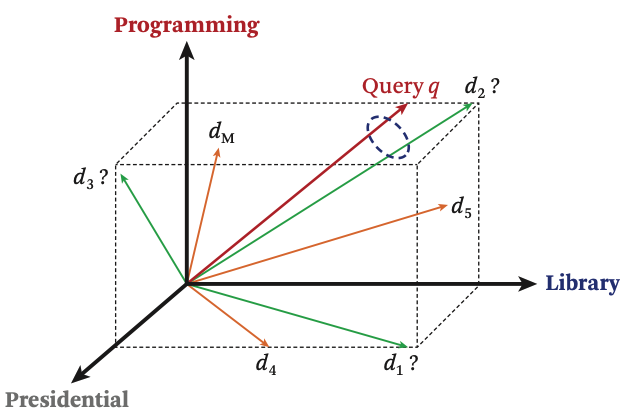
\includegraphics[width=0.7\textwidth]{fotos/17.png}
\caption{}
\label{fig:4.6}
\end{figure}

Un ejemplo se muestra en el panel izquierdo de la figura \ref{fig:4.6}. Se muestran tres clases gaussianas de igual tamaño con vectores de media específicos de la clase y una matriz de covarianza común. Las tres elipses representan regiones que contienen el 95\% de la probabilidad para cada una de las tres clases. Las líneas discontinuas son las fronteras de decisión de Bayes. En otras palabras, representan el conjunto de valores $x$ para los cuales $\delta_k(x) = \delta_\ell(x)$; es decir,
\begin{equation}
x^T \Sigma^{-1} \mu_k - \frac{1}{2} \mu_k^T \Sigma^{-1} \mu_k = x^T \Sigma^{-1} \mu_\ell - \frac{1}{2} \mu_\ell^T \Sigma^{-1} \mu_\ell
\label{eq:4.20}
\end{equation}

\noindent que puede reescribirse como
\begin{equation}
x^T \Sigma^{-1} (\mu_k - \mu_\ell) = \frac{1}{2} (\mu_k^T \Sigma^{-1} \mu_k - \mu_\ell^T \Sigma^{-1} \mu_\ell)
\label{eq:4.20.1}
\end{equation}

para $k \neq l$. (El término $\log(\pi_k)$ de (\ref{eq:4.19}) ha desaparecido porque cada una de las tres clases tiene el mismo número de observaciones de entrenamiento; es decir, $\pi_k$ es el mismo para cada clase). Nótese que hay tres líneas que representan las fronteras de decisión de Bayes porque hay tres pares de clases entre las tres clases. Es decir, una frontera de decisión de Bayes separa la clase 1 de la clase 2, una separa la clase 1 de la clase 3, y una separa la clase 2 de la clase 3. Estas tres fronteras de decisión de Bayes dividen el espacio de predictores en tres regiones. El clasificador de Bayes clasificará una observación según la región en la que se encuentre. \\

Una vez más, se necesita estimar los parámetros desconocidos $\mu_1, \ldots, \mu_K$, $\pi_1, \ldots, \pi_K$, y $\Sigma$; las fórmulas son similares a las utilizadas en el caso unidimensional, dadas en (\ref{eq:4.15}). Para asignar una nueva observación $X = x$, LDA inserta estas estimaciones en (\ref{eq:4.19}) y clasifica a la clase para la cual $\hat{\delta}_k(x)$ es mayor. Nótese que en (\ref{eq:4.19}) $\delta_k(x)$ es una función lineal de $x$; es decir, la regla de decisión LDA depende de $x$ solo a través de una combinación lineal de sus elementos. Una vez más, esta es la razón del término ``lineal'' en LDA. \\

En el panel derecho de la figura \ref{fig:4.6}, se muestran 20 observaciones extraídas de cada una de las tres clases, y las fronteras de decisión LDA resultantes se muestran como líneas negras sólidas. En general, las fronteras de decisión LDA están bastante cerca de las fronteras de decisión de Bayes, mostradas nuevamente como líneas discontinuas. Las tasas de error de prueba para los clasificadores de Bayes y LDA son 0.0746 y 0.0770, respectivamente. Esto indica que LDA está funcionando bien en estos datos. Las tasas de error de entrenamiento suelen ser más bajas que las tasas de error de prueba, que son la cantidad real de interés. La razón es que se ajustan específicamente los parámetros de nuestro modelo para que funcionen bien en los datos de entrenamiento. Cuanto mayor sea la relación de parámetros $p$ con el número de muestras $n$, más se espera que este sobreajuste juegue un papel. \\

En la práctica, un clasificador binario como este puede cometer dos tipos de errores: puede asignar incorrectamente a un individuo que incumple a la categoría de no incumplimiento, o puede asignar incorrectamente a un individuo que no incumple a la categoría de incumplimiento. A menudo es de interés determinar cuál de estos dos tipos de errores se están cometiendo. Una matriz de confusión es una forma conveniente de mostrar esta información. \\

LDA está tratando de aproximar el clasificador de Bayes, que tiene la tasa de error total más baja de todos los clasificadores (si el modelo gaussiano es correcto). Es decir, el clasificador de Bayes producirá el menor número posible de observaciones mal clasificadas, independientemente de la clase de la que provengan los errores. Algunos errores de clasificación resultarán de asignar incorrectamente a un cliente que no incumple a la clase de incumplimiento, y otros resultarán de asignar incorrectamente a un cliente que incumple a la clase de no incumplimiento. En contraste, una compañía de tarjetas de crédito podría desear particularmente evitar clasificar incorrectamente a un individuo que incumplirá, mientras que clasificar incorrectamente a un individuo que no incumplirá, aunque aún debe evitarse, es menos problemático. Es posible modificar LDA para desarrollar un clasificador que satisfaga mejor las necesidades de la compañía de tarjetas de crédito. \\

El clasificador de Bayes funciona asignando una observación a la clase para la cual la probabilidad posterior $p_k(X)$ es mayor. En el caso de dos clases, esto equivale a asignar una observación a la clase \textit{default} si
\begin{equation}
\Pr(\text{default = Yes} | X) > 0.5
\label{eq:4.21}
\end{equation}

Por lo tanto, el clasificador de Bayes, y por extensión LDA, usa un umbral del 50\% para la probabilidad posterior de \textit{default} para asignar una observación a la clase de incumplimiento. Sin embargo, si preocupa predecir incorrectamente el estado de incumplimiento para los individuos que incumplen, entonces se puede considerar bajar este umbral. Por ejemplo, se podría etiquetar a cualquier cliente con una probabilidad posterior de incumplimiento superior al 20\% a la clase de incumplimiento. En otras palabras, en lugar de asignar una observación a la clase \textit{default} si (\ref{eq:4.21}) se cumple, se podría asignar una observación a esta clase si
\begin{equation}
\Pr(\text{default = Yes} | X) > 0.2
\label{eq:4.22}
\end{equation}

Usar un umbral de 0.5, como en (\ref{eq:4.21}), minimiza la tasa de error general. Esto es de esperar, ya que el clasificador de Bayes usa un umbral de 0.5 y se sabe que tiene la tasa de error general más baja. Pero cuando se usa un umbral de 0.5, la tasa de error entre los individuos que incumplen es bastante alta (línea discontinua azul). A medida que se reduce el umbral, la tasa de error entre los individuos que incumplen disminuye constantemente, pero la tasa de error entre los individuos que no incumplen aumenta. Variar el umbral del clasificador cambia su tasa de verdaderos positivos y su tasa de falsos positivos. Estas también se llaman la sensibilidad y uno menos la especificidad del clasificador. \\
\subsection{Análisis discriminante cuadrático}

Como se ha discutido, LDA asume que las observaciones dentro de cada clase se extraen de una distribución gaussiana multivariante con un vector de media específico de la clase y una matriz de covarianza común a todas las $K$ clases. El análisis discriminante cuadrático (QDA) proporciona un enfoque alternativo. Al igual que LDA, el clasificador QDA resulta de asumir que las observaciones de cada clase se extraen de una distribución gaussiana, e insertar estimaciones para los parámetros en el teorema de Bayes para realizar la predicción. Sin embargo, a diferencia de LDA, QDA asume que cada clase tiene su propia matriz de covarianza. Es decir, asume que una observación de la $k$-ésima clase es de la forma $X \sim N(\mu_k, \Sigma_k)$, donde $\Sigma_k$ es una matriz de covarianza para la $k$-ésima clase. Bajo esta suposición, el clasificador de Bayes asigna una observación $X = x$ a la clase para la cual
\begin{align}
\delta_k(x) &= - \frac{1}{2} (x - \mu_k)^T \Sigma_k^{-1} (x - \mu_k) -\frac{1}{2} \log|\Sigma_k| + \log(\pi_k) \notag \\
&= - \frac{1}{2} x^T \Sigma_k^{-1} x + x^T \Sigma_k^{-1} \mu_k - \frac{1}{2} \mu_k^T \Sigma_k^{-1} \mu_k - \frac{1}{2} \log|\Sigma_k| + \log(\pi_k)
\label{eq:4.23}
\end{align}

es mayor. Entonces, el clasificador QDA implica insertar estimaciones para $\Sigma_k$, $\mu_k$, y $\pi_k$ en (\ref{eq:4.23}), y luego asignar una observación $X = x$ a la clase para la cual esta cantidad es mayor. A diferencia de (\ref{eq:4.19}), la cantidad $x$ aparece como una función cuadrática en (\ref{eq:4.23}). Aquí es donde QDA obtiene su nombre. \\

Elegir LDA o QDA radica en el equilibrio entre \textit{bias} y varianza. Cuando hay $p$ predictores, estimar una matriz de covarianza requiere estimar $p(p+1)/2$ parámetros. QDA estima una matriz de covarianza separada para cada clase, para un total de $Kp(p+1)/2$ parámetros. Con 50 predictores, esto es un múltiplo de 1225, lo cual es una gran cantidad de parámetros. Al asumir en su lugar que las $K$ clases comparten una matriz de covarianza común, el modelo LDA se vuelve lineal en $x$, lo que significa que hay $Kp$ coeficientes lineales para estimar. En consecuencia, LDA es un clasificador mucho menos flexible que QDA, y por lo tanto tiene una varianza sustancialmente menor. Esto puede llevar potencialmente a un mejor rendimiento de predicción. Pero hay un compromiso: si la suposición de LDA de que las $K$ clases comparten una matriz de covarianza común es incorrecta, entonces LDA puede sufrir de alto \textit{bias}. En términos generales, LDA tiende a ser una mejor opción que QDA si hay relativamente pocas observaciones de entrenamiento y por lo tanto reducir la varianza es crucial. En contraste, se recomienda QDA si el conjunto de entrenamiento es muy grande, de modo que la varianza del clasificador no sea una preocupación importante, o si la suposición de una matriz de covarianza común para las $K$ clases es claramente insostenible. \\

\begin{figure}[h]
\centering
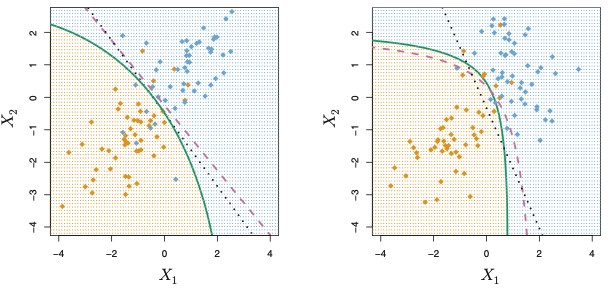
\includegraphics[width=0.7\textwidth]{fotos/18.png}
\caption{Izquierda: Las fronteras de decisión de Bayes (línea discontinua púrpura), LDA (línea punteada negra) y QDA (línea sólida verde) para un problema de dos clases con $\Sigma_1 = \Sigma_2$. El sombreado indica la regla de decisión de QDA. Dado que la frontera de decisión de Bayes es lineal, es más precisamente aproximada por LDA que por QDA. Derecha: Los detalles son los mismos que en el panel izquierdo, excepto que $\Sigma_1 \neq \Sigma_2$. Dado que la frontera de decisión de Bayes es no lineal, es más precisamente aproximada por QDA que por LDA.}
\label{fig:4.9}
\end{figure}

La figura \ref{fig:4.9} ilustra el rendimiento de LDA y QDA en dos escenarios. En el panel izquierdo, las dos clases gaussianas tienen una correlación común de 0.7 entre $X_1$ y $X_2$. Como resultado, la frontera de decisión de Bayes es lineal y es aproximada con precisión por la frontera de decisión de LDA. La frontera de decisión de QDA es inferior, porque sufre de mayor varianza sin una disminución correspondiente en el \textit{bias}. En contraste, el panel derecho muestra una situación en la que la clase naranja tiene una correlación de 0.7 entre las variables y la clase azul tiene una correlación de $-0.7$. Ahora la frontera de decisión de Bayes es cuadrática, y por lo tanto QDA aproxima más precisamente esta frontera que LDA.
\chapter{Evaluación y selección de modelos}\label{Chapter4} 
% chktex-file 8
% chktex-file 12
% chktex-file 13
% chktex-file 44

Lo mas importante del curso. 

\begin{itemize}
\item Empezamos por regresion. Tenemos una variable de salida $Y$ que toma valores en un ontinuo y con p predictores-. Modelamos con una funcion y añadimos el temrino de error. Siempre tendremos este error. nosotros determinamos la $\hat{Y}$ con $\hat{f}$. El error cuadratico medio es la media de los errores al cuadrado.
\item Como evaluamos el error de entrenamineto, que metricas, etc. En ridge, el parametro es beta, loque aprende el modelo. El coeficiente de regularizacion, es decir, $\lambda$, es el hiperparámetro, se lo damos nosotros. No free lunch teorem. algo muy importante!
\item Empezamos a evaluar la calidad del ajuste. No dice nada relevante. $R^2$ no le gusta mucho a el. Esta metrica primero calcula el eror que obtendria el sistema de aprendizake que se nos puede ocurrir: dar como salida la media de todos nuestros ejemplos (TSS da como salida la media). Luego calcula la diferencia entre eso y la suma de los cuadrados y normalizandolo. HAciendolo peor que la media esta metrica daria negativa incluso (muy dificil). Gusta porque el error se acota entre 0 (dificil bajarla) y 1. No le gusta a el porque es engañoso, los problemas no son comparables y por tanto los valores de la metrica tampoco. Se suele usar el MSE porque no depende del numero de ejemplos. 

menor MSE train no garantiza menor MSE test! Interesamos en el modelo con mejor error de test. 
\item Diapositiva importante !! Sobreaprendizaje y subaprendizaje. EL modleo verde es el de menor MSE de train pero el azul el de menor MSE de test. Flexibilidad = complejidad de modelo, mejor se va a adaptar a los datos del modelo. Error de train y test alto = subaprendizaje, modelo demasiado simple para nuestros datos. Error de train bajo y test alto = sobreaprendizaje, modelo demasiado complejo. Al hacer exploracion hay que intentar conseguir siempre la curva para llegar al subaprendizaje y sobreaprendizaje, asi aseguramos que barremos todo el rango de hiperparametros.
\item Tanto el amarillo como el azul son mas o menos buenos. A igualdad, preferimos modelos sencillos, ya que tiene mayor capacidad de generalizacion. 
\item Habria que explorar mas modelos, se sobreajuste
\item Dos formas de estimar el error de test (1) teoricamente, cogemos un subconjunto datos y calculamos el error de test sobre otro conjunto de entrenamiento. (2) lo mimos ??? La varianza nos dice cuanto cambia la funcion si cambiamos algunos de los datos de entrenamiento. Modelos sencillos tienen poca varianza, variar un dato no lo cambia mucho. Modelos complejos tienen mucha varianza, variar un dato lo cambia mucho.
\item Bias: def. el modelo amarillo de la 2.9 tiene mucho bias, modelo verde casi nulo.  
\item La curva roja es el error total, es decir, suma el bias, avarianza y el error irreducible.Minimos cuadrados es un modelo sobreaprendido. La flexibilidad de ridge y laso va entonces con $1/\lambda$, a mayor lambda menor lambda el modelo tiende al sobreaprendizaje. 
\item Ahora lo mismo peroapra clasificacion. PAra medir la calidad de modelo se suele usar el error de clasificacion: contamos el numero de ejemplos en los que nos estamos equivocando. No profundizara en el clasificador de bayes. LDA hace una aproximacion al clasificador de bayes porque no se conocen las probabilidades; LDA asume una distribucion normal.
\item Como tenemos el ejemplo, si podemos usar el de Bayes
\item Asumimos un problema de clasificacion binario. Ahi podemos construir una matriz de confusion. $N^*$ son los negativos que estima el modelo ($N \neq N^*$).
\item La curva ROC se usa para medir la calidad de clasificadores binarios 
\end{itemize}

\section{Selección de subconjuntos} \label{sec:4.1}

\subsection{Selección del mejor subconjunto}

Para hacer la selección del mejor subconjunto, se debe ajustar una regresión de mínimos cuadrados distinta para cada combinación de los $p$ predictores. Esto es, se ajustan todos los $p$ modelos que contienen exactamente un predictor, los $\binom{p}{2} = p(p-1)/2$ modelos que contienen exactamente dos predictores, y así sucesivamente. Luego, se selecciona el mejor modelo. \\

El problema viene en elegir el mejor de entre las $2^p$ posibilidades consideradas. Esto se suele hacer en dos etapas:
\begin{enumerate}
\item Sea $\mathcal{M}_0$ el modelo nulo que no contiene ningún predictor. Este modelo predice la media de la muestra para cada observación.
\item Para $k = 1, 2, \ldots, p$:
\begin{enumerate}
\item Ajustar todos los $\binom{p}{k}$ modelos que contienen exactamente $k$ predictores.
\item Elegir el mejor modelo entre los $\binom{p}{k}$ modelos, y llamarlo $\mathcal{M}_k$. Aquí, ``mejor'' se refiere a tener el menor RSS o, equivalentemente, el mayor $R^2$. Tras esto, el problema se reduce de $2^p$ posibilidades a $p+1$. 
\end{enumerate}
\item Elegir un único ``mejor'' modelo de entre $\mathcal{M}_0, \dots, \mathcal{M}_p$ usando predicción de error validada de forma cruzada, $C_p$ (AIC), BIC, o $R^2$ ajustado.
\end{enumerate}

Para elegir el mejor modelo hay que elegir entre los $p+1$ modelos $\mathcal{M}_i$, con $i = 0, \dots, p$. Hay que tener en cuenta que el RSS de estos modelos decrece de forma monótona, mientras que el $R^2$ aumenta de forma monótona. Por tanto, si se usa estos estadísticos para elegir el mejor modelo, siempre se acabará con un modelo que incluya todas las variables. El problema es que un RSS bajo o un $R^2$ alto indica un modelo con un error de entrenamiento bajo, mientras que lo que se quiere es elegir un modelo con un error de \textit{test} bajo. Por tanto, en el paso 3, se usa la predicción de error validada de forma cruzada, $C_p$, BIC o $R^2$ ajustado para elegir entre $\mathcal{M}_0, \mathcal{M}_1, \dots, \mathcal{M}_p$. 

\subsection{Selección por pasos}

Por motivos computacionales, la selección del mejor subconjunto no sirve para $p$ grandes, caso donde puede sufrir de porblemas estadísticos. Cuando mayor sea el espacio de búsqueda, mayor será la posibilidad de encontrar modelos que ajusten bien el conjunto de entrenamiento, aunque no tenga buen poder predictivo. Entonces, un gran espacio de búsqueda puede conducir a \textit{overfitting} y una gran variación de los coeficientes estimados. Los modelos de selección por pasos exploran un conjunto restringido de modelos, por lo que resultan una buena alterantiva. 

\subsubsection{Selección por pasos hacia adelante}

Este método resulta más eficiente computacionalmente que la selcción del mejor subconjunto. Este método comienza con un modelo que no contenga predictores, y va añadiendo predictores al modelo, uno a uno, hasta que todos los predictores están dentro del modelo. En particular, en cada paso, se añade la variable que dé la mayor mejora al ajuste. Formalmente:
\begin{enumerate}
\item Sea $\mathcal{M}_0$ el modelo nulo, que no contiene predictores.
\item Para $k = 0, \dots, p-1$:
\begin{enumerate}
\item Considera los $p-k$ modelos que aumentan los predictores en $\mathcal{M}_k$ con un predictor adicional.
\item Elige el mejor entre estos $p-k$ modelos y lo denota $\mathcal{M}_{k+1}$. Aquí el ``mejor'' es aquel con menor RSS o mayor $R^2$. 
\end{enumerate}
\item Elige el mejor modelo entre $\mathcal{M}_0, \dots, \mathcal{M}_p$ usando predicción de error validada de forma cruzada, $C_p$ (AIC), (BIC) o $R^2$ ajustado.
\end{enumerate}

A diferencia de la selección del mejor subconjunto, que necesita ajustar $2^p$ modelos, la selección por pasos hacia adelante necesita ajustar un modelo nulo, junto con $p-k$ modelos en la iteración k-ésima para $k = 0, \dots, p-1$. Esto resulta en un total de $1 \sum_{k=0}^{p-1}(p-k) = 1 + p(p+1)/2$ modelos. \\

En el segundo paso, el apartado (b), se debe elegir el mejor modelo entre los $p-k$ modelos que aumentan $\mathcal{M}_k$ con un predictor adicional. Esto se puede hacer eligiendo el modelo con menor RSS o mayor $R^2$. Sin embargo, en el paso 3, se debe elegir el mejor modelo entre un conjunto de modelos con diferente número de variables. Esto es más complicado y se discute en la sección 6.1.3. \\

La ventaja computacional del método de selección por pasos hacia adelante sobre la selección del mejor subconjunto es clara. Aunque el método de selección por pasos hacia adelante tiende a funcionar bien en la práctica, no está garantizado que encuentre el mejor modelo posible de entre los $2^p$ modelos que contienen subconjuntos de los $p$ predictores. Por ejemplo, sea un conjunto de datos con $p = 3$ predictores, el mejor modelo de una variable contiene $X_1$, y el mejor modelo de dos variables contiene $X_2$ y $X_3$. Entonces, la selección por pasos hacia adelante no seleccionará el mejor modelo de dos variables, porque $\mathcal{M}_1$ contendrá $X_1$, por lo que $\mathcal{M}_2$ también debe contener $X_1$ junto con una variable adicional. \\

La selección por pasos hacia adelante se puede aplicar incluso en el caso de gran dimensión donde $n < p$, aunque en este caso, solo se pueden construir submodelos $M_0, \dots, M_{n-1}$, ya que cada submodelo se ajusta utilizando mínimos cuadrados, lo que no dará una solución única si $p \geq n$.

\subsubsection{Selección por pasos hacia atrás}

Este método comienza con el modelo de mínimos cuadrados que contiene todos los predictores, y luego elimina uno a uno los predictores que menos contribuyen al ajuste. Formalmente:
\begin{enumerate}
\item Sea $\mathcal{M}_p$ el modelo completo que contiene los $p$ predictores.
\item Para $k = p, p-1, \dots, 1$:
\begin{enumerate}
\item Considera los $k$ modelos que contienen todos menos uno de los predictores en $\mathcal{M}_k$, para un total de $k-1$ predictores.
\item Elige el mejor entre estos $k$ modelos y lo denota $\mathcal{M}_{k-1}$. Aquí el ``mejor'' es aquel con menor RSS o mayor $R^2$.
\end{enumerate}
\item Elige el mejor modelo entre $\mathcal{M}_0, \dots, \mathcal{M}_p$ usando predicción de error validada de forma cruzada, $C_p$ (AIC), (BIC) o $R^2$ ajustado.
\end{enumerate}

La selección por pasos hacia atrás también necesita ajustar $1 + p(p+1)/2$ modelos, al igual que la selección por pasos hacia adelante, y también puede aplicarse para el caso en el que $p$ es demasiado grande como para aplicar la selección del mejor conjunto. Este método tampoco garantiza encontrar el mejor modelo de entre los $2^p$ posibles. \\

La selección por pasos hacia detrás no se puede aplicar en el caso en el que $n < p$, ya que el modelo completo no se puede ajustar en este caso.

\subsubsection{Modelos híbridos}

En general, no se obtienen los mismos modelos de selección por pasos hacia adelante y hacia atrás. Como alternativa, se pueden considerar versiones híbridas de selección por pasos hacia adelante y hacia atrás, en las que las variables se agregan al modelo secuencialmente, de manera análoga a la selección hacia adelante, pero después de agregar cada nueva variable, el método puede eliminar cualquier variable que ya no proporcione una mejora en el ajuste del modelo. Este enfoque intenta imitar más de cerca la selección del mejor subconjunto, mientras mantiene las ventajas computacionales de la selección por pasos hacia adelante y hacia atrás.

\subsection{Selección del modelo óptimo}

\begin{equation}
C_p = \frac{1}{n}(RSS + 2d\hat{\sigma}^2)
\end{equation}

\begin{equation}
AIC = \frac{1}{n\hat{\sigma}^2}(RSS + 2d\hat{\sigma}^2)
\end{equation}

\begin{equation}
BIC = \frac{1}{n}(RSS + \log(n)d\hat{\sigma}^2)
\end{equation}

\begin{equation}
R^2_{\text{ajustado}} = 1 - \frac{RSS/(n-d-1)}{TSS/(n-1)}
\end{equation}

\subsubsection{Validación y validación cruzada}

\subsubsection{Reduciendo de error}

En situacion de subaprendizaje, añadir mas datos no va a ayudar. PAra resolverlo hay que ir a un modelo más complejo. Podemos añadir caracteristicas o variables nuevas y/o decrementar la regularización (en ridge lasso seria disminuir $\lambda$) (este es el más directo y sencillo). \\

En situacion de sobreaprendizaje, añadir mas datos si que ayuda. Hay que ir a un modelo más simple. Podemos eliminar caracteristicas o variables y/o incrementar la regularización .
\chapter{K vecinos más próximos}\label{Chapter5} 
% chktex-file 8
% chktex-file 12
% chktex-file 13
% chktex-file 44

En teoría, siempre se desearía predecir respuestas cualitativas usando el clasificador de Bayes. Pero para datos reales, no se conoce la distribución condicional de $Y$ dado $X$, por lo que calcular el clasificador de Bayes es imposible. Por lo tanto, el clasificador de Bayes sirve como un estándar inalcanzable contra el cual comparar otros métodos. Muchos enfoques intentan estimar la distribución condicional de $Y$ dado $X$, y luego clasificar una observación dada a la clase con la mayor probabilidad estimada. Uno de estos métodos es el clasificador de $K$-vecinos más próximos (KNN). Sea un entero positivo $K$ y una observación de prueba $x_0$, el clasificador KNN primero identifica los $K$ puntos en los datos de entrenamiento que están más cerca de $x_0$, representados por $\mathcal{N}_0$. Luego estima la probabilidad condicional para la clase $j$ como la fracción de puntos en $\mathcal{N}_0$ cuyos valores de respuesta son iguales a $j$:
\begin{equation}
\Pr(Y = j | X = x_0) = \frac{1}{K} \sum_{i \in \mathcal{N}_0} I(y_i = j)
\label{eq:2.12}
\end{equation}

Finalmente, KNN aplica la regla de Bayes y clasifica la observación de prueba $x_0$ a la clase con la mayor probabilidad. \\

\begin{figure}[h]
\centering
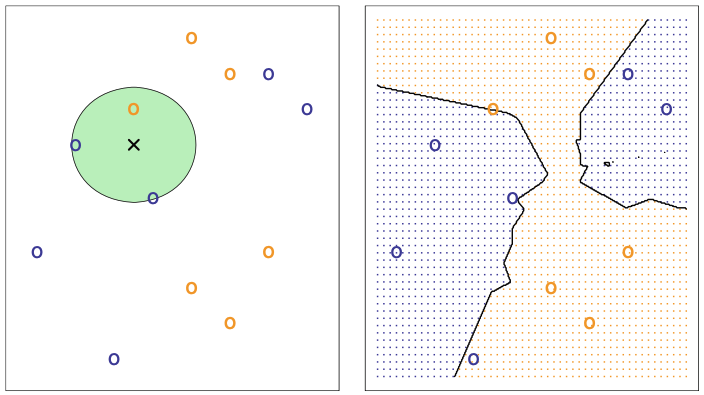
\includegraphics[width=0.6\textwidth]{fotos/10.png}
\caption{El enfoque KNN, usando $K = 3$, se ilustra en una situación simple con seis observaciones azules y seis observaciones naranjas. Izquierda: una observación de prueba para la cual se desea una etiqueta de clase predicha se muestra como una cruz negra. Se identifican los tres puntos más cercanos a la observación de prueba, y se predice que la observación de prueba pertenece a la clase que ocurre con mayor frecuencia, en este caso azul. Derecha: La frontera de decisión KNN para este ejemplo se muestra en negro. La cuadrícula azul indica la región en la cual una observación de prueba será asignada a la clase azul, y la cuadrícula naranja indica la región en la cual será asignada a la clase naranja.}
\label{fig:2.14}
\end{figure}

La figura \ref{fig:2.14} proporciona un ejemplo del enfoque KNN. En el panel izquierdo, se ha graficado un pequeño conjunto de datos de entrenamiento que consiste en seis observaciones azules y seis naranjas. El objetivo es hacer una predicción para el punto etiquetado con la cruz negra. Supongamos que se elige $K = 3$. Entonces KNN primero identificará las tres observaciones que están más cerca de la cruz. Este vecindario se muestra como un círculo. Consiste en dos puntos azules y un punto naranja, resultando en probabilidades estimadas de $2/3$ para la clase azul y $1/3$ para la clase naranja. Por lo tanto, KNN predecirá que la cruz negra pertenece a la clase azul. En el panel derecho de la figura \ref{fig:2.14} se ha aplicado el enfoque KNN con $K = 3$ en todos los valores posibles para $X_1$ y $X_2$, y se ha dibujado la correspondiente frontera de decisión KNN. A pesar de que es un enfoque muy simple, KNN puede producir clasificadores que están sorprendentemente cerca del clasificador de Bayes óptimo. La figura \ref{fig:2.15} muestra la frontera de decisión KNN, usando $K = 10$, cuando se aplica al conjunto de datos simulado más grande de la figura \ref{fig:2.13}. Nótese que aunque el clasificador KNN no conoce la distribución verdadera, la frontera de decisión KNN está muy cerca de la del clasificador de Bayes. La tasa de error de prueba usando KNN es 0.1363, que está cerca de la tasa de error de Bayes de 0.1304. \\

\begin{figure}[H]
\centering
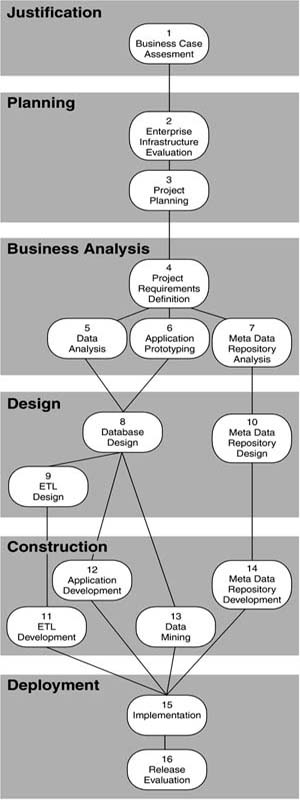
\includegraphics[width=0.4\textwidth]{fotos/11.png}
\caption{La curva negra indica la frontera de decisión KNN en los datos de la figura \ref{fig:2.13}, usando $K = 10$. La frontera de decisión de Bayes se muestra como una línea discontinua púrpura. Las fronteras de decisión KNN y de Bayes son muy similares.}
\label{fig:2.15}
\end{figure}

\begin{figure}[H]
\centering
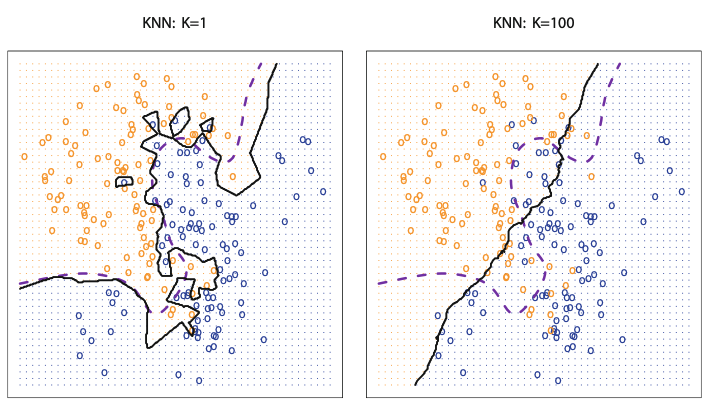
\includegraphics[width=0.7\textwidth]{fotos/12.png}
\caption{Una comparación de las fronteras de decisión KNN (curvas negras sólidas) obtenidas usando $K = 1$ y $K = 100$ en los datos de la figura \ref{fig:2.13}. Con $K = 1$, la frontera de decisión es excesivamente flexible, mientras que con $K = 100$ no es suficientemente flexible. La frontera de decisión de Bayes se muestra como una línea discontinua púrpura.}
\label{fig:2.16}
\end{figure}

La elección de $K$ tiene un efecto drástico en el clasificador KNN obtenido. La figura \ref{fig:2.16} muestra dos ajustes KNN a los datos simulados de la figura \ref{fig:2.13}, usando $K = 1$ y $K = 100$. Cuando $K = 1$, la frontera de decisión es excesivamente flexible y encuentra patrones en los datos que no corresponden a la frontera de decisión de Bayes. Esto corresponde a un clasificador que tiene bajo sesgo pero muy alta varianza. A medida que $K$ crece, el método se vuelve menos flexible y produce una frontera de decisión que es casi lineal. Esto corresponde a un clasificador de baja varianza pero alto sesgo. En este conjunto de datos simulado, ni $K = 1$ ni $K = 100$ dan buenas predicciones: tienen tasas de error de prueba de 0.1695 y 0.1925, respectivamente. \\

Al igual que en el contexto de regresión, no hay una relación estrecha entre la tasa de error de entrenamiento y la tasa de error de prueba. Con $K = 1$, la tasa de error de entrenamiento de KNN es 0, pero la tasa de error de prueba puede ser bastante alta. En general, a medida que se usan métodos de clasificación más flexibles, la tasa de error de entrenamiento disminuirá pero la tasa de error de prueba puede no hacerlo. En la figura \ref{fig:2.17} se han graficado los errores de prueba y de entrenamiento de KNN como una función de $1/K$. A medida que $1/K$ aumenta, el método se vuelve más flexible. Como en el contexto de regresión, la tasa de error de entrenamiento disminuye consistentemente a medida que aumenta la flexibilidad. Sin embargo, el error de prueba exhibe una forma característica de U, disminuyendo al principio (con un mínimo en aproximadamente $K = 10$) antes de aumentar nuevamente cuando el método se vuelve excesivamente flexible y sobreajusta. \\

En ambos contextos, de regresión y clasificación, elegir el nivel correcto de flexibilidad es crítico para el éxito de cualquier método de aprendizaje estadístico. El equilibrio entre sesgo y varianza, y la resultante forma de U en el error de prueba, pueden hacer de esta una tarea difícil. 

\begin{figure}[H]
\centering
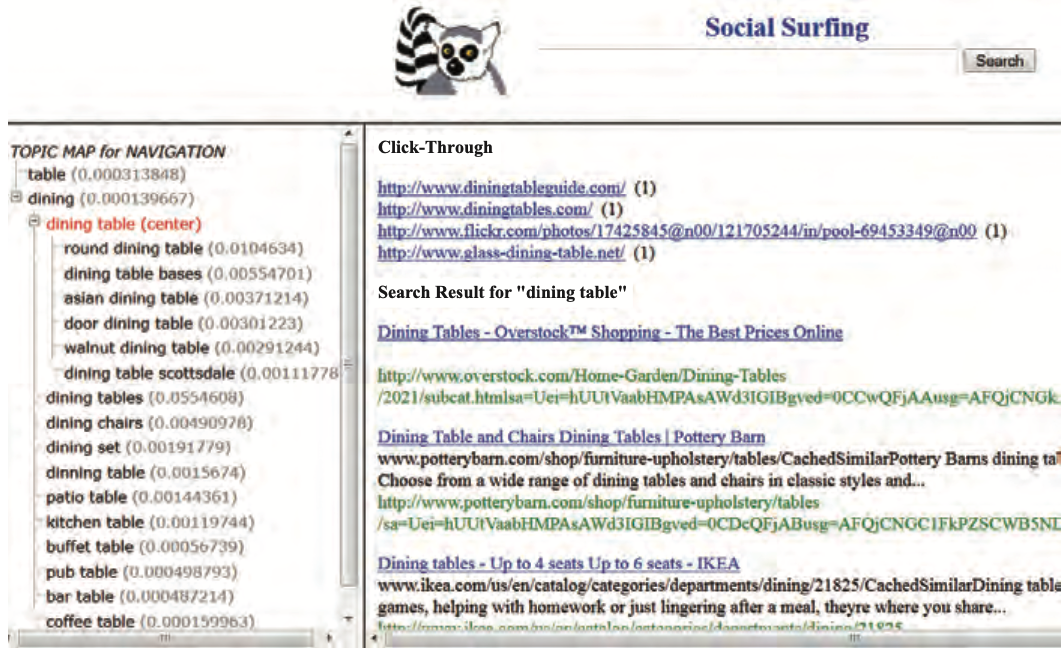
\includegraphics[width=0.6\textwidth]{fotos/13.png}
\caption{La tasa de error de entrenamiento KNN (azul, 200 observaciones) y la tasa de error de prueba (naranja, 5,000 observaciones) en los datos de la figura \ref{fig:2.13}, a medida que el nivel de flexibilidad (evaluado usando $1/K$) aumenta, o equivalentemente, a medida que el número de vecinos $K$ disminuye. La línea discontinua negra indica la tasa de error de Bayes. La irregularidad de las curvas se debe al pequeño tamaño del conjunto de datos de entrenamiento.}
\label{fig:2.17}
\end{figure}
\chapter{Representaciones avanzadas de texto}\label{Chapter6} 
% chktex-file 8
% chktex-file 12
% chktex-file 13
% chktex-file 44

HAce 10 años empezo una revolucion en el campo de la representacion de texto con Word2vec. Pasamos de representaciones sprse a representaciones densas de mebeddngs que capturan mejor la semantica y significado del texto. 

CHATGPT tiene un impacto social enorme


Esta revolucion que cambia y por que cambia. Lo tradicional en claisifcacion automatica, el paradigma, se tiene un traing data etiqueta, se lo doy al sistema aprende y puedo poner en produccion. El cuello de botella es que necesito etiquetas en el training data. Da capacidades limitadas de compresion de lenguaje, ya que para ello tendria que meter gran cantidad de formas de decir lo mismo, incluir toda la casuistica.

Primera vuelta de tuerca, preentrenar y finetune. LOs modelos se preentrenan: cogemos una gran cantidad de datos (no toda la web pero casi) y jugando al juego de ocultar palabras (haciendo masking) y predecir la palabra oculta. Si lo dice mal, la penalizo. Si lo hace bien, consigo un modelo que entiende bien el lenguaje, la semantica, otros tipos de conocimientos sobre el mundo. Esto es autoentrenamiento sin etiquetado.  


Una vez entrenado, lo ajusto y personalizo para mi tarea con el fine tune (adaptation). 





La idea clave de los embbeding es construir automaticamente un representacion de las palabras donde las palabras que son similares conceptualemente estan cerca en el espacio vectorial. Los alrededores de una palabra (izquierda y derecha) son los que determinan el significado de la palabra (ejemplo de tezgüino). Las palabras parecidad van a tener contextos izquierdo y derecho parecidos. Esta es la base teórica para la integración semántica de la representación de las palabras. \\

Un word embedding es una lista, un vector denso de longitud fija. PAra construirlas se puede hacer de muchas formas: por ejemplo, estadísticas de coocurrencia. Esto es un espacio de bajas dimensiones. Muchas veces se aprenden con redes de neuronas. \\

Para que sirve esto? si yo tengo los embeddings de todas las palabras se pueden buscar las palabras cercanas en el espacio embebido para buscar sinonimos, por ejemplo. 

Una estrategia posible es que los embeddings sea la entrada a una red de neuronas para entrenamiento supervisada. Tambien podemos representar el corpus con los embeddings y ver los posibles clusters. 

Los vectores de las palabras admiten operaciones !

Los redes de neuronas. Se coge una red de neuronas y la hago jugar a un juego predictivo de ir escondiendo palabras y que vaya adivinando. Aqui el proceso de backpropagation juega un papel fundamental. Queremos que palabras que significan lo mismo vayan a la misma representación. Otras alternativas son mas algebraicas, usando cuentas de coocurrencia 


Predecir la palabra j-esima dadas las anteriores (tipo gpt). Una red de neuronas que hago esto bien es util. En el ambito de los LLM da un gran conocimiento del mundo, tanto semantico como sintactico y gramatical. 

estos ebeddings no es que se produjera la red de neuronas para darlos, se encontro que era un subproducto de la red de neuronas.

VEamos varios ejemplos

NNLM: Contruyo una red de neuronas para predecir una palabra i esima dada las anteriores y el output layer es la probabilidad de cada palabra en el vocabulario dadas las anteriores. Internamente representa los embeddings del texto. Los mebeddigs son los pesos de la capa de entrada a la capa oculta. (la e simboliza embedding) x coge la representacion de las embeddings, lo mete en una capa interna (h).


WORD2VEC. Embeddings independietnes del contexto, es decir, palabras polisemicas tienen un solo embedding para todos los significados, aquí estas palabras sufren. Esto lo hace leyendo un corpus masivo y de ese (auto)aprendizaje, porque no etiquetamos nada, aprende las palabras. Una forma de predecir es CBOW , predecir una palabra dando las anteriores y posteriores.... Da una representacion distribuida. DEF. 

BERT (la B de Bert es de bidireccional). Embeddings dependiente del contexto, para palabras polisemicas, da un embedding diferente a cada significado.

BERT solo hace encoding (hace todo lo necesario para crear una representación interna del texto), GPT solo decoding (me pasas la representacion al lenguaje que te pido) y otros tienen ambas, por ejemplo T5. CHATGPT ademas esta tuneado para seguir instrucciones; luego se adapta a conversar y genera una representacion de la isntruccion y producirla en el lenguaje que se pida. 


T5: sequence-to-sequence. en funcion e cierto patron de entrada produce cierto aprametro de salida. T5 se utilizan para reranking (ranking hecho con un BM25 o algo clasico), pero con T5 es muy costoso. El T5 aprende de un proceso de enmascaramiento (preeentraenamiento). Mono T5 esta finetuneado con MSMarco, coleccion de pasajes que puso bing. 

count-based models. LSA
No basados en redes neuronales pero igualmente son capaces de generar representaciones densas. La idea del LSA: sabemos el problema de las representaciones sparse (dos sinonimos no guardan relacion) idealmente no querria indexar por palabras, sino por conceptos. El problema es que los conceptos no son explicitos. LSA usa la matriz originales y transformarla a un espacio de conceptos usando una estrategia de coocurrencia cpn metodos algebraicos. 

HAL:  busca todos los contextos (ventanas de aparicion de las palabras en los corpus) y analiza la cuenta de coocurrencia entre esa palabra y los contextos. 

COAL: poco detalle

LR-MVL: un poco mas moderno. Si tiene en cuenta contexto izquierdo y derecho. 

GLOVE: mejora sobre estrategias como Word2Vec (problema mira las apariciones de las palabras en el corpus, no usa informacion global). GLOVE tiene en cuenta informacion de estadísticas globales, no en las coocurrencias individuales sino globales.

FINAL REMARKS. CHALLENGES.

OOV- muchos modelos de embeddings no gestionan palabras no vistas anteriormente. 
\chapter{Redes neuronales}\label{Chapter7} 
% chktex-file 8
% chktex-file 12
% chktex-file 13
% chktex-file 44

Veremos redes neuronales poco profundas (no más de 2 capas ocultas). La idea básica es transformar un conjunto de variables capa a capa hasta llegar a un conjunto de variables fácilmente separables o ``regresables'' por la ultima capa. El resultado del pesado se pasa por una funcion de activacion no lineal. El peso $w_{ij}$ conecta la neurona j de la capa l con la neurona i de la capa l+1. No contamos el bias como neurona, asiq ue en el ejemplo que pone hay 3. El bias es un vector siempre, con dimension $\text{neuronas en esa capa} \times 1$. PAra el caso de la capa de entrada, la activacion es directametne la entrada. 

\section{Introducción}

Consideremos un problema de aprendizaje supervisado donde tenemos acceso a ejemplos de entrenamiento etiquetados $(x^{(i)}, y^{(i)})$. Las redes neuronales ofrecen una forma de definir una hipótesis compleja y no lineal $h_{W,b}(x)$, con parámetros $W, b$ que podemos ajustar a nuestros datos. \\

Para describir las redes neuronales, comenzaremos describiendo la red neuronal más simple posible, una que comprende una sola ``neurona''. Utilizaremos el diagrama \ref{fig:7.1} para denotar una sola neurona

\begin{figure}[H]
\centering
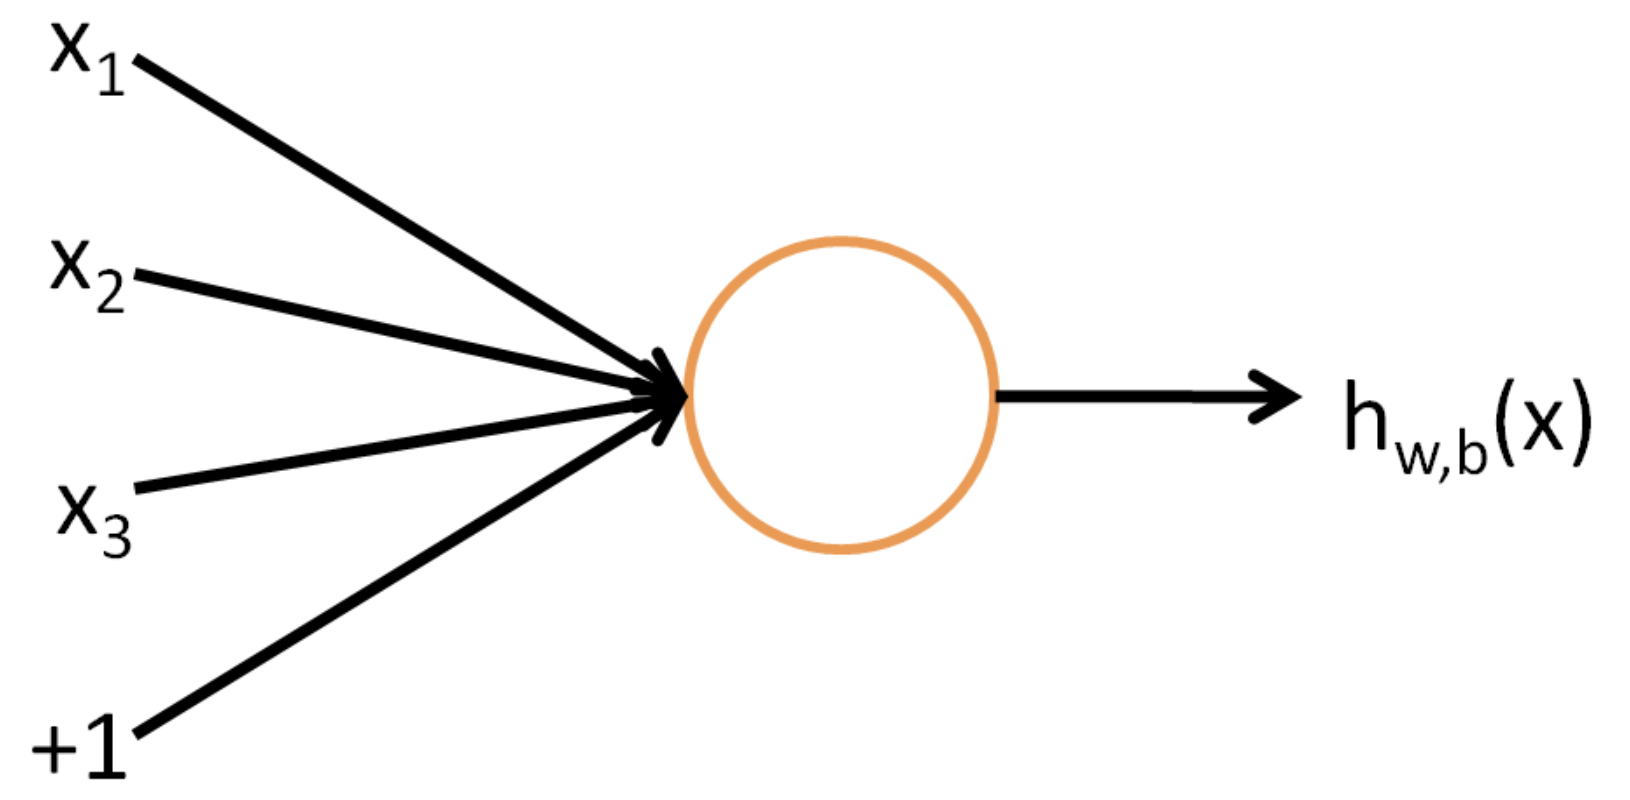
\includegraphics[width=0.4\textwidth]{fotos/40.png}
\caption{Diagrama de una neurona simple}
\label{fig:7.1}
\end{figure}

Esta ``neurona'' es una unidad computacional que toma como entrada $x_1, x_2, x_3$ (y un término de intercepto $+1$; este \textit{bias} no se cuenta como ``neurona''), y produce una salida 
\begin{equation}
h_{W,b}(x) = f(W^T x) = f\left(\sum_{i=1}^{3} W_i x_i + b\right)
\end{equation}

\noindent donde $f: \mathbb{R} \rightarrow \mathbb{R}$ se denomina función de activación. 

\subsection{Función de activación}

\subsubsection{Función sigmoide}

\noindent Aquí, elegiremos $f(\cdot)$ como la función sigmoide:
\begin{equation}
f(z) = \frac{1}{1 + e^{-z}}
\end{equation}

\noindent función acotada entre 0 y 1 también conocida como función logística estándar. Así, nuestra única neurona corresponde exactamente al mapeo de entrada-salida definido por la regresión logística. Una propiedad importante de esta función es que su derivada de puede escribir en términos de la misma función:
\begin{equation}
f'(z) = f(z)(1 - f(z))
\end{equation}

\begin{figure}[h]
\centering
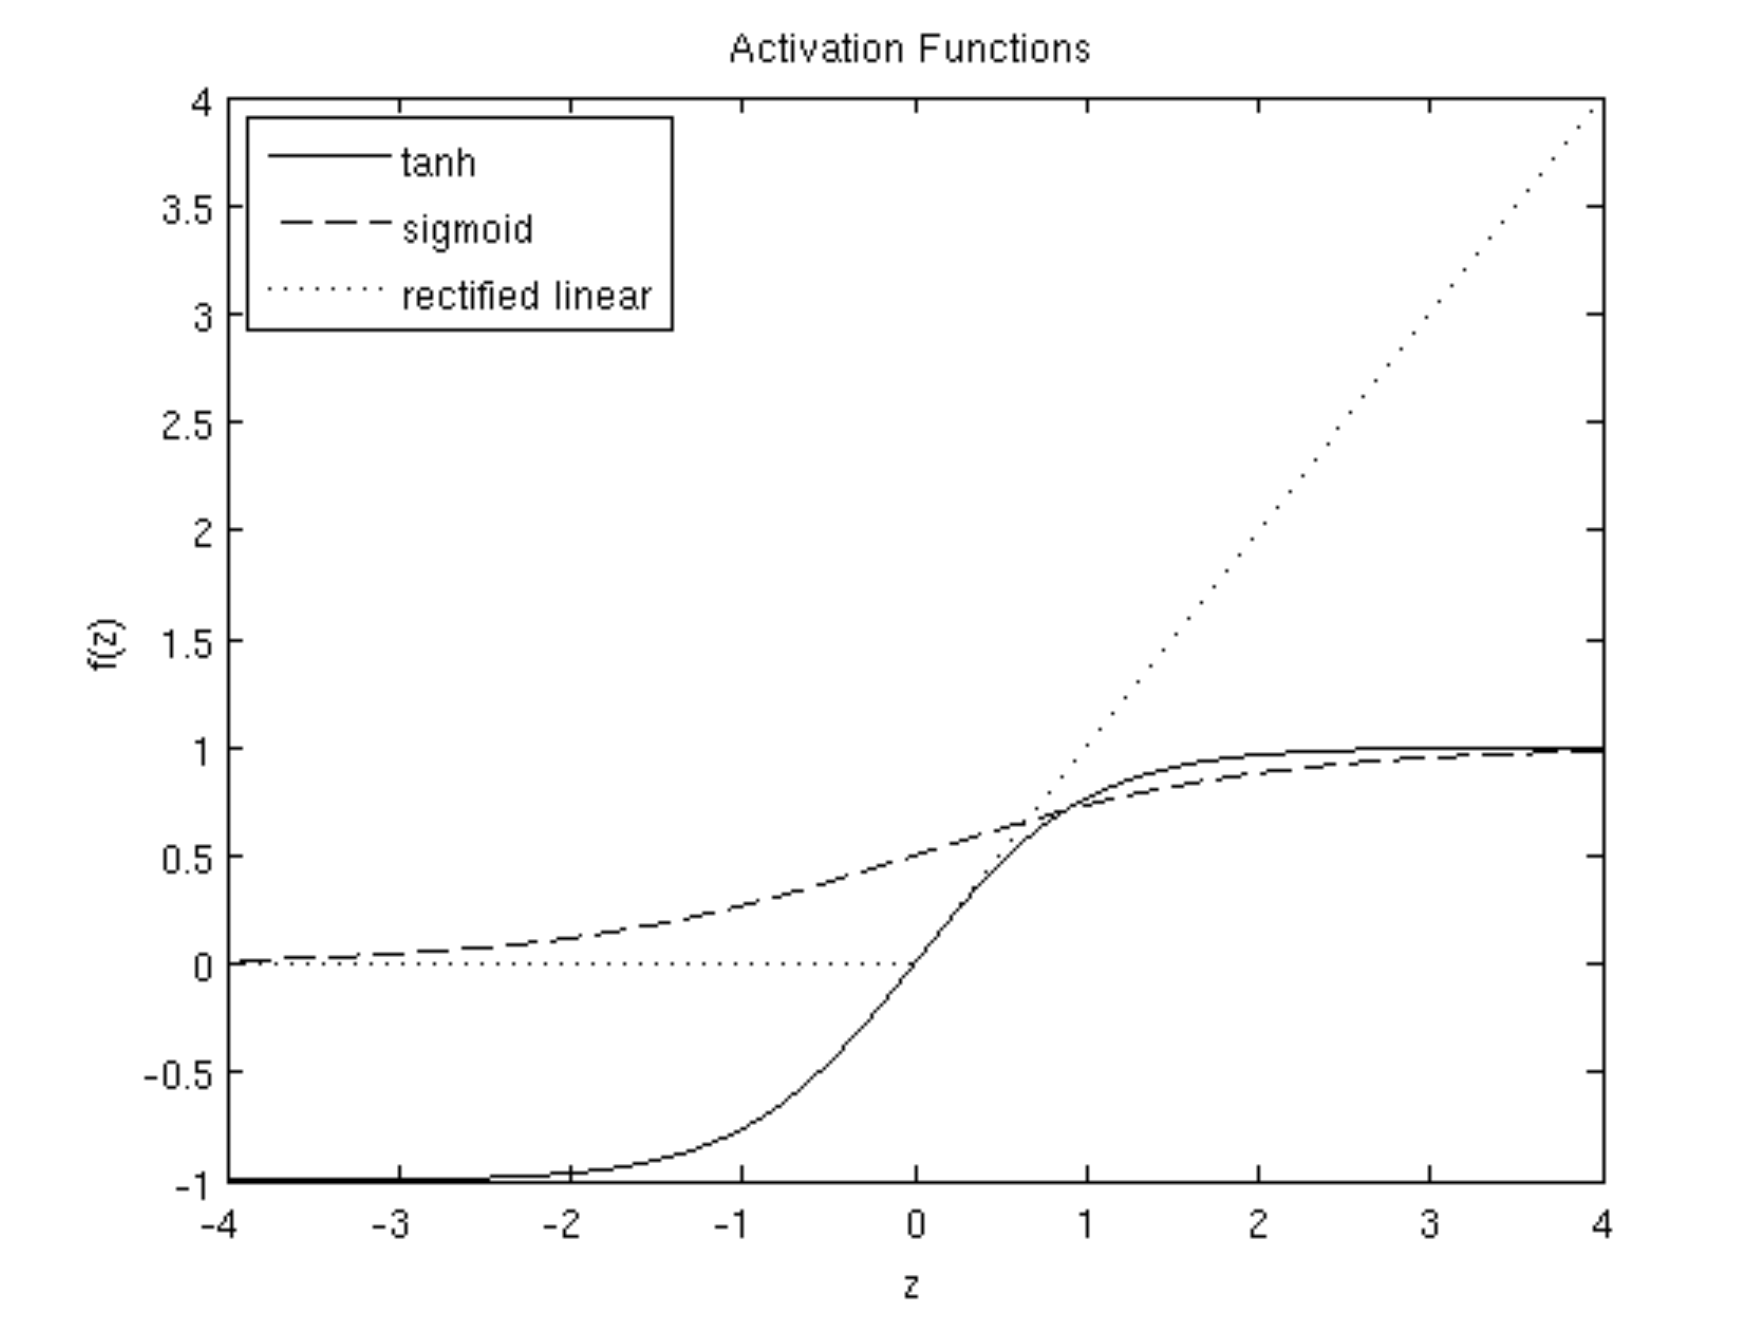
\includegraphics[width=0.6\textwidth]{fotos/41.png}
\caption{Funciones de activación: Sigmoide, tanh y ReLU}
\label{fig:7.2}
\end{figure}

\subsubsection{Tangente hiperbólica}

Aunque usaremos la función sigmoide, vale la pena notar que otra elección común para $f$ es la función tangente hiperbólica, o tanh:
\begin{equation}
f(z) = \tanh(z) = \frac{e^{z} - e^{-z}}{e^{z} + e^{-z}}
\end{equation}

La función $\tanh(z)$ es una versión reescalada de la sigmoide, y su rango de salida es $[-1, 1]$ en lugar de $[0,1]$. La derivada de esta función toma la forma $f'(z) = 1 - (f(z))^2$. 

\subsubsection{Función lineal rectificada ReLU}

Una función de activación diferente, la función lineal rectificada (ReLU), a menudo funciona mejor en la práctica para redes neuronales profundas. Esta función de activación es diferente de la sigmoide y la tanh porque no está acotada ni es continuamente diferenciable. La función de activación lineal rectificada se define como:
\begin{equation}
f(z) = \max(0, z)
\end{equation}

La función lineal rectificada es lineal por tramos y se satura exactamente en $0$ cuando la entrada $z$ es menor que $0$. Su derivada (gradiente) es 0 para $z<0$ y 1 para $z > 0$. El gradiente no está definido en $z = 0$, aunque esto no causa problemas en la práctica porque promediamos el gradiente sobre muchos ejemplos de entrenamiento durante la optimización.

\subsubsection{Funciones gaussianas de base radial}

El modelo de redes neuronales de funciones de base radial (RBF) es un modelo no lineal que utiliza funciones de base radial como funciones de activación. Las funciones de base radial son funciones que dependen solo de la distancia radial al origen, por lo que su valor es el mismo en todos los puntos que equidistan del origen. Sean matrices de covarianza cualesquiera, las funciones de base radial se definen como:
\begin{equation}
f_j(\mathbf{z}) = \exp\left\{-\frac{1}{2}(\mathbf{z} - \boldsymbol{\mu}_j)^T \boldsymbol{\Sigma}_j^{-1}(\mathbf{z} - \boldsymbol{\mu}_j)\right\}
\end{equation}

Como las matrices de covarianza son simétricas, se tiene que cada función de base radial tiene $d(d + 3)/2$ parámetros independientes ajustables, donde $d$ es la dimensión del espacio de entrada. \\


\section{Modelo de red neuronal}

Una red neuronal se construye conectando muchas ``neuronas'', de modo que la salida de una neurona puede ser la entrada de otra. Por ejemplo, la figura \ref{fig:7.3} muestra una pequeña red neuronal:

\begin{figure}[h]
\centering
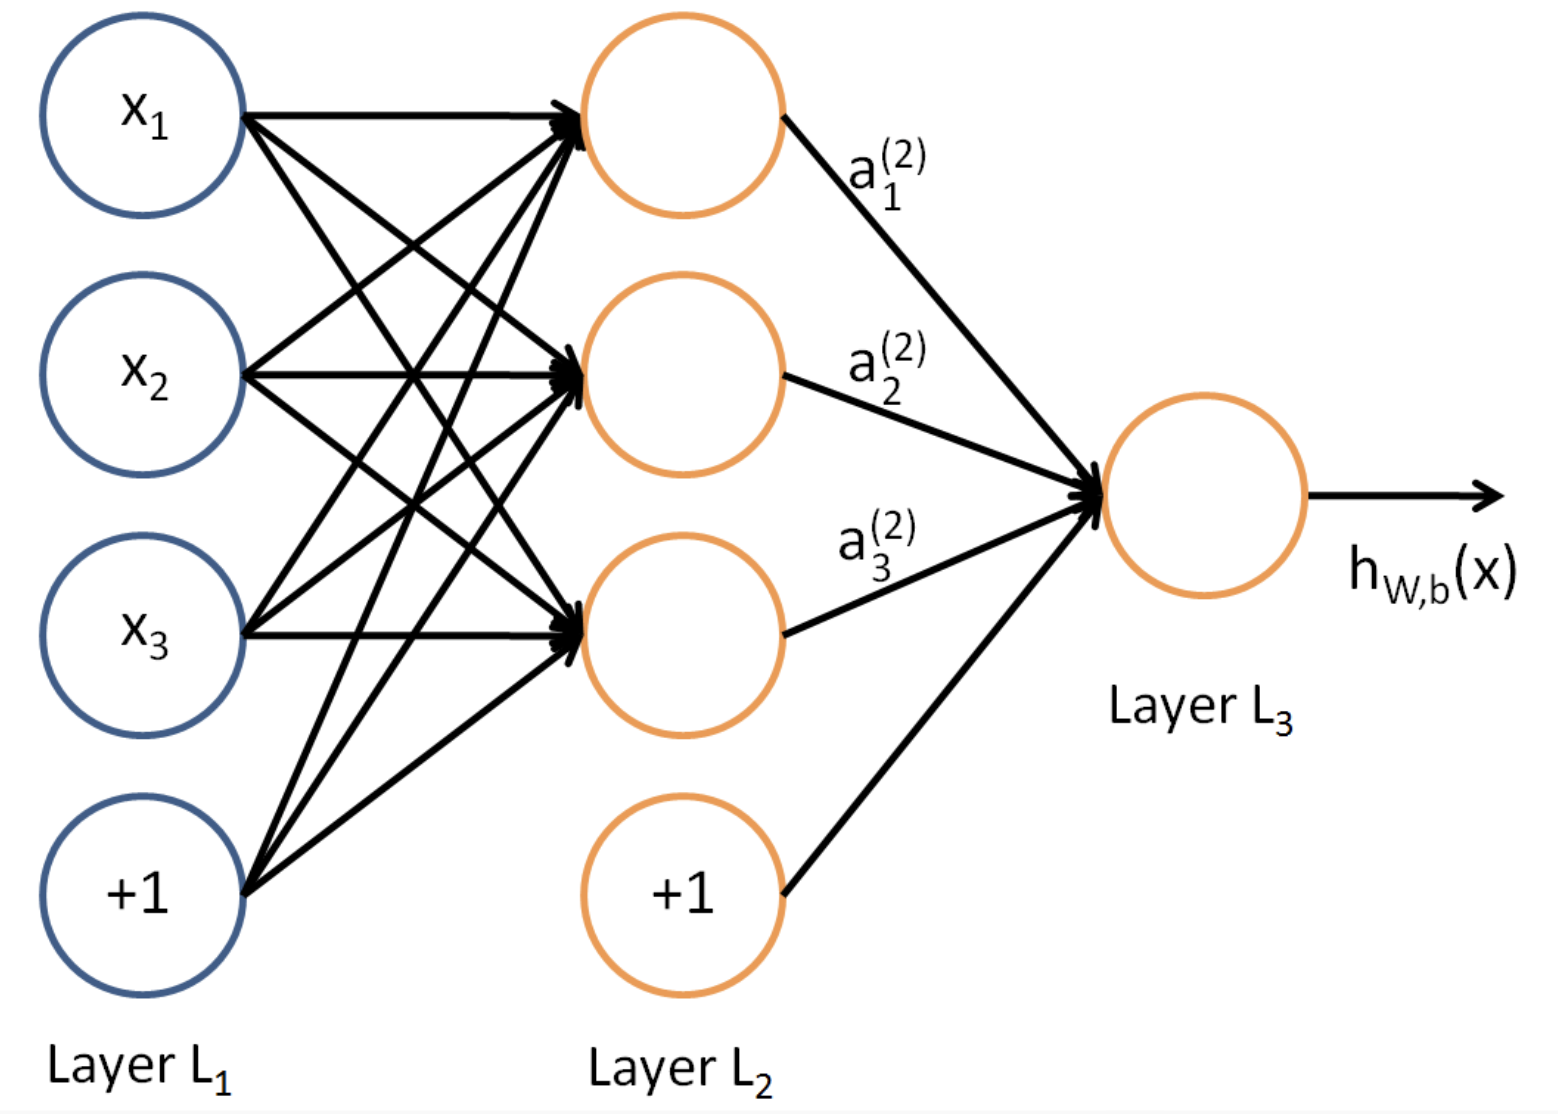
\includegraphics[width=0.5\textwidth]{fotos/42.png}
\caption{Ejemplo de una red neuronal pequeña}
\label{fig:7.3}
\end{figure}

En esta figura, hemos utilizado círculos para denotar también las entradas a la red. Los círculos etiquetados como ``+1'' se llaman unidades de sesgo y corresponden al término de intercepto. La capa más a la izquierda de la red se llama capa de entrada, y la capa más a la derecha la capa de salida (que, en este ejemplo, tiene solo una unidad). La capa intermedia de nodos se llama capa oculta, porque sus valores no se observan en el conjunto de entrenamiento. También decimos que nuestro ejemplo de red neuronal tiene 3 unidades de entrada (sin contar la unidad de sesgo), 3 unidades ocultas y 1 unidad de salida. \\

Denotaremos $n_l$ como el número de capas en nuestra red; por lo tanto, $n_l = 3$ en nuestro ejemplo. Etiquetamos la capa $l$ como $L_l$, por lo que la capa $L_1$ es la capa de entrada y la capa $L_{n_l}$ la capa de salida. \\

Nuestra red neuronal tiene parámetros $(W, b) = (W^{(1)}, b^{(1)}, W^{(2)}, b^{(2)})$, donde escribimos $W_{ij}^{(l)}$ para denotar el parámetro (o peso) asociado con la conexión entre la unidad $j$ en la capa $l$ y la unidad $i$ en la capa $l+1$ (nota el orden de los índices). Además, $b_i^{(l)}$ es el sesgo asociado con la unidad $i$ en la capa $l+1$. Así, en nuestro ejemplo, tenemos $W^{(1)} \in \mathbb{R}^{3 \times 3}$ y $W^{(2)} \in \mathbb{R}^{1 \times 3}$. Note que las unidades de sesgo no tienen entradas ni conexiones entrantes, ya que siempre sacan el valor $+1$; en nuestro ejemplo $b^{(1)} \in \mathbb{R}^{3 \times 1}$ y $b^{(2)} \in \mathbb{R}^{1 \times 1}$. También denotamos $s_l$ como el número de nodos en la capa $l$ (sin contar la unidad de sesgo). \\

Escribiremos $a^{(l)}_i$ para denotar la activación (es decir, el valor de salida) de la unidad $i$ en la capa $l$. Para $l = 1$, también usamos $a^{(1)}_i = x_i$ para denotar la $i$-ésima entrada. En lo sucesivo, también denotamos $z^{(l)}_i$ como la suma ponderada total de entradas a la unidad $i$ en la capa $l$, incluyendo el término de sesgo,  
\begin{equation}
z_i^{(l+1)} = \sum_{j=1}^{s_l} W_{ij}^{(l)} a_j^{(l)} + b_i^{(l)}
\end{equation}

\noindent de modo que $a^{(l)}_i = f(z^{(l)}_i)$. Dado un conjunto fijo de parámetros $W, b$, nuestra red neuronal define una hipótesis $h_{W,b}(x)$ que produce un número real. Específicamente, el cómputo que esta red neuronal representa se da por:

\begin{align}
a_1^{(2)} &= f\left(W_{11}^{(1)} x_1 + W_{12}^{(1)} x_2 + W_{13}^{(1)} x_3 + b_1^{(1)}\right) \\
a_2^{(2)} &= f\left(W_{21}^{(1)} x_1 + W_{22}^{(1)} x_2 + W_{23}^{(1)} x_3 + b_2^{(1)}\right) \\
a_1^{(2)} &= f\left(W_{31}^{(1)} x_1 + W_{32}^{(1)} x_2 + W_{33}^{(1)} x_3 + b_3^{(1)}\right) \\
h_{W, b}(x) &= a_1^{(3)} = f\left(W_{11}^{(2)} a_1^{(2)} + W_{12}^{(2)}a_2^{(2)} + W_{13}^{(2)} a_3^{(2)} + b_1^{(2)}\right)
\end{align}

Nótese que esto se presta fácilmente a una notación más compacta. Específicamente, si extendemos la función de activación $f(\cdot)$ para que se aplique a vectores de manera elemento a elemento (es decir, $f([z_1, z_2, z_3]) = [f(z_1), f(z_2), f(z_3)]$), entonces podemos escribir las ecuaciones anteriores de manera más compacta como:
\begin{align}
z^{(2)} &= W^{(1)} x + b^{(1)} \\
a^{(2)} &= f(z^{(2)}) \\
z^{(3)} &= W^{(2)} a^{(2)} + b^{(2)} \\
h_{W,b}(x) &= a^{(3)} = f(z^{(3)})
\end{align}

Llamamos a este paso propagación hacia adelante (\textit{forward propagation}). Más generalmente, recordando que también usamos $a^{(1)} = x$ para denotar los valores de la capa de entrada, dadas las activaciones $a^{(l)}$ de la capa $l$, podemos calcular las activaciones $a^{(l+1)}$ de la capa $l+1$ como:
\begin{align}
z^{(l+1)} &= W^{(l)} a^{(l)} + b^{(l)} \\
a^{(l+1)} &= f(z^{(l+1)})
\end{align}

Al organizar nuestros parámetros en matrices y utilizando operaciones de álgebra lineal vectorial, podemos aprovechar rutinas rápidas de álgebra lineal para realizar cálculos en nuestra red de manera eficiente. \\

\section{Arquitecturas}

Hasta ahora, nos hemos centrado en un ejemplo de red neuronal, pero también se pueden construir redes neuronales con otras arquitecturas (es decir, patrones de conectividad entre neuronas), incluyendo aquellas con múltiples capas ocultas. Las capas pueden estar conectadas densamente, como en nuestro ejemplo, o pueden tener conexiones más dispersas (locales, \textit{locally connected}), en cuyo caso se pueden compartir los pesos. \\

La elección más común es una red de $n_l$ capas donde la capa $1$ es la capa de entrada, la capa $n_l$ es la capa de salida, y cada capa $l$ está densamente conectada a la capa $l+1$. En este contexto, para computar la salida de la red, podemos calcular sucesivamente todas las activaciones en la capa $L_2$, luego en la capa $L_3$, y así sucesivamente, hasta la capa $L_{n_l}$, utilizando las ecuaciones anteriores que describen el paso de propagación hacia adelante. Este es un ejemplo de una red neuronal \textit{feedforward}, ya que el grafo de conectividad no tiene bucles ni ciclos dirigidos. \\

Las redes neuronales también pueden tener múltiples unidades de salida. Por ejemplo, en la figura \ref{fig:7.4} hay una red con dos capas ocultas $L_2$ y $L_3$ y dos unidades de salida en la capa $L_4$.

\begin{figure}[h]
\centering
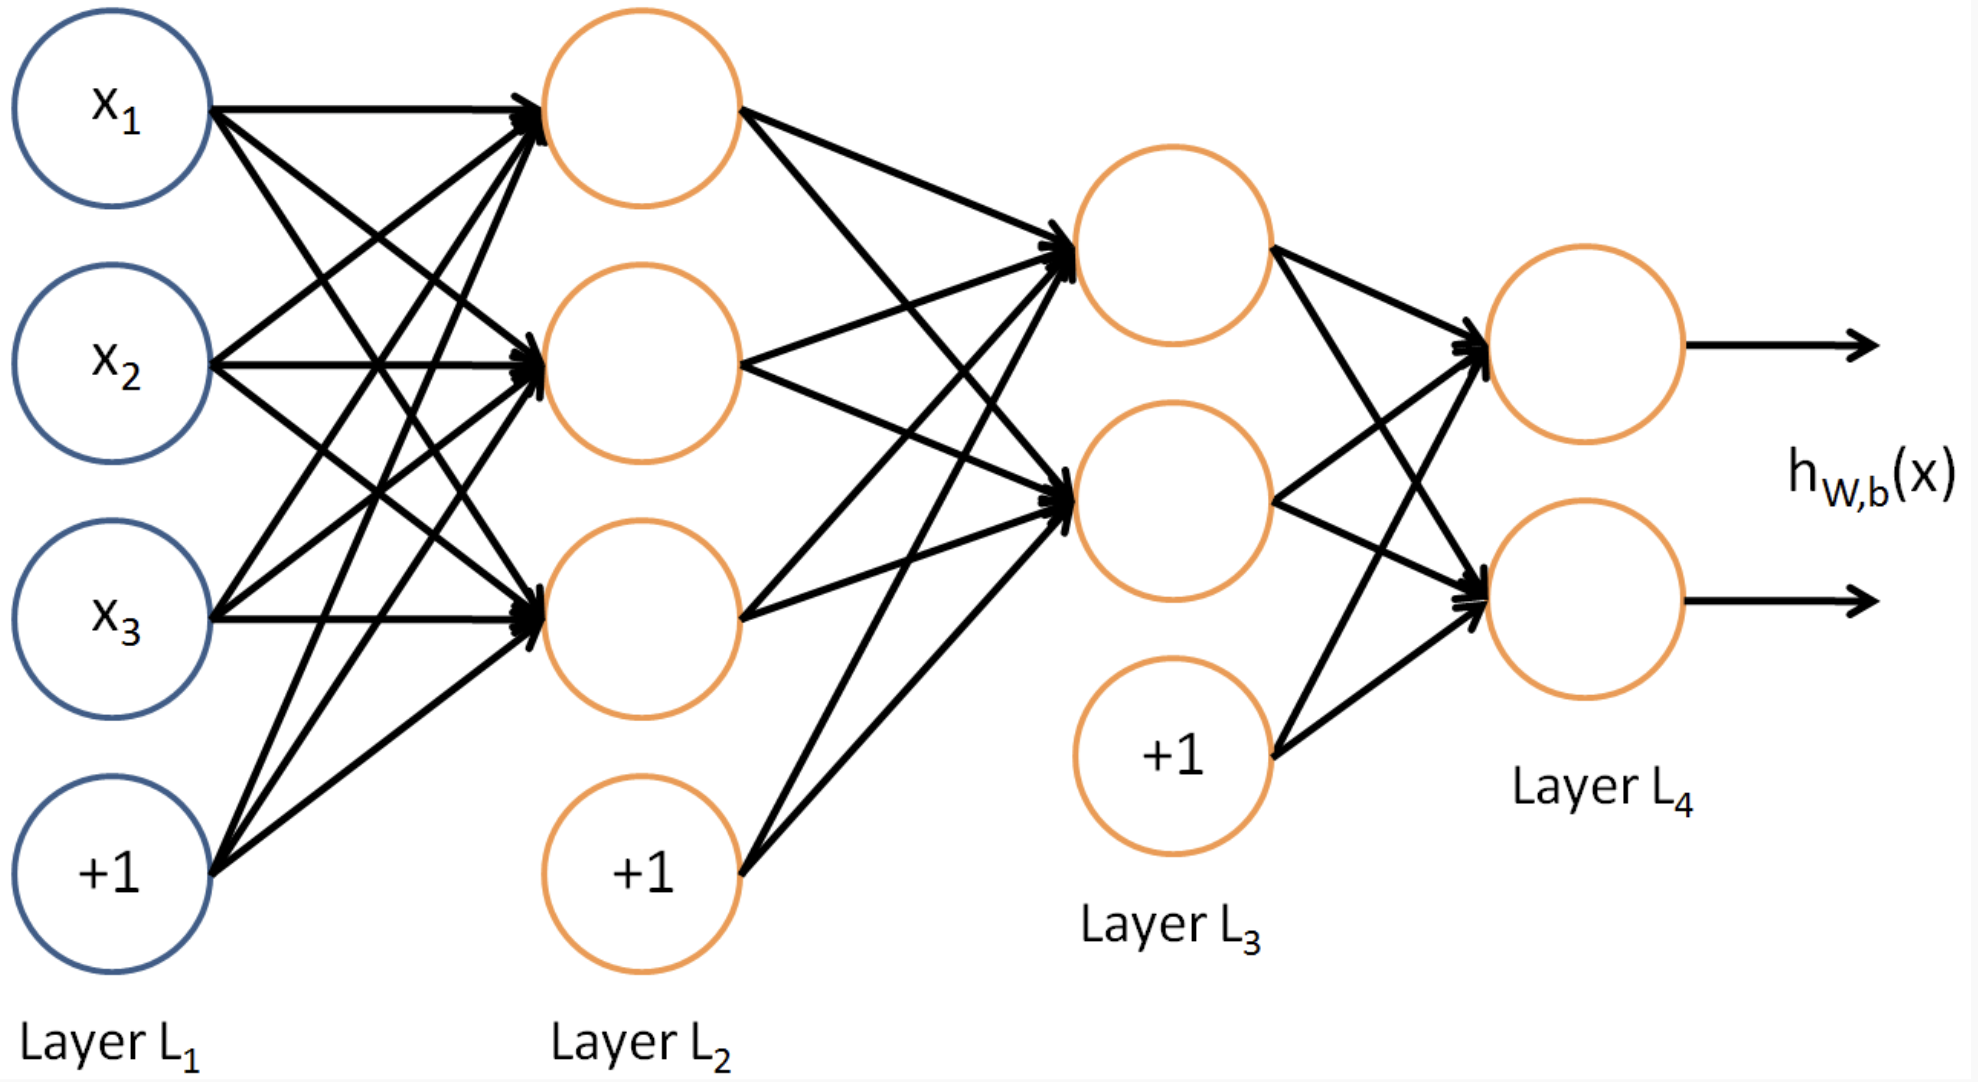
\includegraphics[width=0.6\textwidth]{fotos/43.png}
\caption{Red neuronal con múltiples capas ocultas y múltiples unidades de salida.}
\label{fig:7.4}
\end{figure}

Para entrenar esta red, necesitaríamos ejemplos de entrenamiento $(x^{(i)}, y^{(i)})$ donde $y^{(i)} \in \mathbb{R}^2$. Este tipo de red es útil si hay múltiples salidas que te interesa predecir. Por ejemplo, en una aplicación de diagnóstico médico, el vector $x$ podría proporcionar las características de entrada de un paciente, y las diferentes salidas $y_i$ podrían indicar la presencia o ausencia de diferentes enfermedades. \\

Dependiendo del tipo de problema a afrontar, se toman ciertas consideraciones generales: 
\begin{itemize}
\item Regresión.
\begin{itemize}
\item Una salida por cada variable de salida.
\item La función de salida es generalmente la función identidad.
\item Estandarización de los datos (entradas y salidas), ya que el rango depende de la función de activación.
\end{itemize}
\item Clasificación. 
\begin{itemize}
\item Para clasificación binaria, se utiliza una única unidad de salida y la sigmoide como función de salida.
\item Para una clasificación de $K$ clases, se utilizan $K$ unidades de salida: \textit{encoding} $[1 \; 0 \; 0 \; 0]^T$, $[0 \; 1 \; 0 \; 0]^T$, $[0 \; 0 \; 1 \; 0]^T$, $[0 \; 0 \; 0 \; 1]^T$.
\item La función de salida es generalmente la función \textit{softmax}.
\begin{equation}
f(z_i^{(l)}) = \frac{\exp(z_i^{(l)})}{\sum_{j = 1}^K \exp(z_j^{(l)})}
\end{equation}
\begin{example}
Salida de la función \textit{softmax} para un caso de clasificación de 3 clases: bicicleta, coche y camión.
\begin{table}[H]
\centering
\begin{tabular}{ccccc}
\hline \hline
 & $z_i$ & $\exp(z_i)$ & $f(z_i)$ & Prob. correctas \\ \hline \hline
Bicicleta & $-0.2$ & $0.8$ & $0.2$ (2\%) & $0.00$ \\
Coche & $3.6$ & $36.6$ & $0.75$ (75\%) & $1.00$ \\
Camión & $2.4$ & $11.0$ & $0.23$ (23\%) & $0.00$ \\ \hline 
\end{tabular}
\end{table}
\end{example}
\end{itemize}
\end{itemize}

\section{Funciones de coste o error}

Sea un conjunto de entrenamiento $\{(x^{(1)}, y^{(1)}), \ldots, (x^{(m)}, y^{(m)})\}$. 

\subsection{Logartimo negativo de la verosimilitud}

Intuitivamente, queremos maximizar la probabilidad de verosimilitud sobre los datos de entrenamiento; esto es, cada punto de datos se asume que se genera a partir de la misma distribución de probabilidad
\begin{equation}
\mathcal{P} = \prod_{i = 1}^m p(x_i, y_i) = \prod_{i = 1}^m p(y_i \mid x_i) p(x_i)
\end{equation}

Sin embargo, el producto de probabilidades en poco estable numéricamente (se obtienen valores muy pequeños), por lo que se suele usar el logaritmo negativo de la verosimilitud como función de coste (a minimizar):
\begin{equation}
J = -\log \mathcal{P} = -\sum_{i = 1}^m \log p(y_i \mid x_i) - \log \sum_{i = 1}^m p(x_i) = -\sum_{i = 1}^m \log p(y_i \mid x_i)
\end{equation}

\subsection{Suma del error cuadrático}

\noindent Si se asume que la distribución de los datos es gaussiana,
\begin{equation}
p(y \mid x) = \prod_{i = 1}^m \frac{1}{(2\pi \sigma^2)^{1/2}} \exp\left(-\frac{(h(x_i) - y_i)^2}{2\sigma^2}\right)
\end{equation} 

\noindent se puede usar la suma del error cuadrático como función de coste:
\begin{equation}
J = \frac{1}{2} \sum_{i = 1}^m (h(x_i) - y_i)^2
\end{equation}

\subsection{Entropía cruzada}

\subsubsection{Entropía cruzada binaria}

\noindent Para problemas de clasificación binaria, se puede usar la entropía binaria cruzada como función de coste:
\begin{itemize}
\item Para una sola unidad de salida: $p(\mathcal{C}_1 \mid x_i) = h(x_i)$ y $p(\mathcal{C}_2 \mid x_i) = 1 - h(x_i)$
\item La función de salida es la sigmoide, por lo que se interpreta como una probabilidad.
\end{itemize}

\noindent En caso de tener más de una unidad de salida,
\begin{equation}
p(y_i \mid x_i) = (h(x_i))^y_i (1 - h(x_i))^{1 - y_i}
\end{equation}

\noindent y la función de coste es
\begin{equation}
J = -\sum_{i = 1}^m \left(y_i \log h(x_i) + (1 - y_i) \log (1 - h(x_i))\right)
\end{equation}

Esta función de error es mínima cuando las predicciones del modelo coinciden con las etiquetas reales, esto es $h(x_i) = y_i$. La derivada de esta función respecto a la salida del modelo $h(x_i)$ es
\begin{equation}
\frac{\partial J}{\partial h(x_i)} = \frac{h(x_i) - y_i}{h(x_i)(1 - h(x_i))}
\end{equation}

\subsubsection{Entropía cruzada}

\noindent Para problemas de clasificación multiclase ($K$ clases), con clases mutuamente excluyentes, se tiene que 
\begin{align}
p (\mathcal{C}_k \mid x_i) &= h^k(x_i) \\
p (y_i \mid x_i) &= \prod_{k = 1}^K (h^k(x_i))^{y_i^k}
\end{align}

donde el superíndice $k$ simplemente indica la clase $k$-ésima. La función de coste asociada es 
\begin{equation}
J = -\sum_{i = 1}^m \sum_{k = 1}^K y_i^k \log h^k(x_i)
\end{equation}

En el caso de tener $K$ clases mutuamente no excluyentes, se asume independencia en las categorías, esto es
\begin{equation}
p (y_i \mid x_i) = \prod_{k = 1}^K (h^k(x_i))^{y_i^k} (1 - h^k(x_i))^{1 - y_i^k}
\end{equation}

\noindent y la función de error se escribe como 
\begin{equation}
J = -\sum_{i = 1}^m \sum_{k = 1}^K \left(y_i^k \log h^k(x_i) + (1 - y_i^k) \log (1 - h^k(x_i))\right)
\end{equation}

Ambas funciones de coste tienen un mínimo de error en $h^k(x_i) = y_i^k$. Los valores de salida pasan por una \textit{softmax}, por lo que se interpretan como probabilidades.

\begin{example}
Sean tres clases mutuamente excluyentes: bicicleta, coche y camión. Suponemos que la salida de la función \textit{softmax} es 
\begin{table}[H]
\centering
\begin{tabular}{cc}
\hline \hline
Clase & \textit{softmax} \\ \hline \hline
Bicicleta ($k = 1$) & 0.02 \\
Coche ($k = 2$) & 0.75 \\
Camión ($k = 3$) & 0.23 \\ \hline
\end{tabular}
\end{table}

\noindent La función de coste, al ser clases mutuamente excluyentes, es
\begin{equation}
J = -\sum_{i = 1}^m \sum_{k = 1}^K y_i^k \log h^k(x_i)
\end{equation}

\noindent Así, $J = - (0.0 - 0.29 - 0.0) = 0.29$ ya que  
\begin{itemize}
\item $k = 1$: $0 \cdot \log (0.02) = 0.0$
\item $k = 2$: $1 \cdot \log (0.75) = -0.29$
\item $k = 3$: $0 \cdot \log (0.23) = 0.0$
\end{itemize}

Dependiendo de las probabilidades de salida, se obtiene un valor de error distinto que nos indica cuán bien está clasificando el modelo. Supongamos varios casos:
\begin{table}[H]
\centering
\begin{tabular}{cccl}
\hline \hline
Clase real & \textit{softmax}(h) & $J$ &  \\ \hline \hline
Coche & $\{0.02, \textcolor{green}{0.75}, 0.23\}$ & $0.29$ & Buen clasificador \\
Coche & $\{0.00, \textcolor{green}{1.00}, 0.00\}$ & $0.00$ & Clasificador perfecto \\
Camión & $\{0.00, \textcolor{red}{0.75}, 0.25\}$ & $1.39$ & Mal clasificador \\
Camión & $\{0.00, \textcolor{red}{1.00}, 0.00\}$ & $\gg$ & El peor clasificador posible \\
\end{tabular}
\end{table}
\end{example}
\chapter{Arboles}\label{Chapter8} 
% chktex-file 8
% chktex-file 12
% chktex-file 13
% chktex-file 44


En un arbol de decision se tiene muy claro de donde viene la salida (interpretable), pero no puede competir con los mejores modelos de predicción. Solo veremos CART, que vale para regresión y clasificación.

EXAMPLE:

Los menores de 4.5 (estricto) se da el valor directametne. Si es mayor igual de 4.5, analizamos los golpes, si es menos, 6, si es mayor, 6.74. El primer nodo de años divide el eje de años en dos partes (no tienen por qué ser iguales). En el siguiente nodo se divide la parte correspondiente a una de las partes anteriores por el eje Hits. Divides en regiones y cuando una muestra cae en una región, se da la media de los datos de entrenamiento de esa región. La division en años, puede hacerse de tantas formas como años se disponga en los datos. 

REGRESSION TREES:
el tamaño del arbol es el hiperparametro que controlara el subaprendizaje o subaprendizaje del algoritmo (determina el tamaño del arbol). arbol pequeño subapredndio. Buscamos la division de regiones que minimiza la formula del RSS vista.

USAMOS METODOS APROXIMADO. RECURSIVE BINARY SPLITTING.

En cada punto escogemos la mejor variable y el mejor umbral. Decisiones individuales y no globales para que sea computacionalmente mas eficiente. No hay garantia de encontrar el optimo para si una bueno. El criterio es la formaulas que salen ahi para R1 y R2 minimizando ese error. 

\begin{example}
Sea dos variables $X_1 = (-3, -2, 0, 2, 5)$ e $Y = (4, 6, -2, 8, 10)$. Buscamos las posibles particiones para esas variables. En este caso entre los datos (punto medio), $(-2.5, -1, 1, 3.5)$. Cada umbral divide el conjunto en dos regiones, la de la izquierda de los datos y la de la derecha. Habría que calcular los errores, ejemplo con particion en +1. \\

Esta particion nos deja dos regiones $R_1 = \{(-3, 4), (-2, 6), (0, -2)\}$ y $R_2 = \{(2, 8), (5, 10)\}$. Calculamos la media de las salidas de cada región: $\hat{y}_{R_1} = 8/3$ y $\hat{y}_{R_2} = 9$. Calculamos ahora el error
\begin{align}
\underbrace{(4 - 8/3)^2 + (6 - 8/3)^2 + (-2 - 8/3)^2}_{R_1} + \underbrace{(8 - 9)^2 + (10 - 9)^2}_{R_2}
\end{align}
Lo repetimos para los 4 umbrales posibles y nos quedamos con el que minimice el error. Luego repetimos con $X_2$ y nos quedamos con el que minimice el error. Así con todas las variables y umbrales posibles.
\end{example}

Paramos de dividir en una rama cuando se cumple el criterio de parada (esto nos dara por tanto el tamaño del arbol) usamos el tamaño minimo de nodo: cuando en un nodo hay menos de los ejemplos fijados, dejamos de dividirlo. Para sobreaprender, el tamaño de nodo deberá ser pequeño, por lo que el arbol sera grande. Este es el que mejor funciona en general. Unico hiperparametro que usaremos. 

Hay otro criterio para parar: que todas las salidas de un nodo sean las mismas, no tendria sentido seguir dividiendo (este se ve mejor en clasificacion). 

Problema de maxima profundidad, todas las ramas u hojas son del mimso tamaño

Otro se calcula el error de la division y si no mejora en un porcentaje, se para (comparar el error de una region con el error de la division de ambas (sumado obvio con la formula)). Problema: hacer mas divisiones puede mejorar el error, aunque una concreta no lo haga. 


De cada nodo tenemos media y desviacion, por lo que podemos dar confianza ($\pm$) en la prediccion.

PODADO DEL ARBOL (PRUNING):

Probar quitar cada uno de los nodos es ineficiente. Usamos el cost complexity pruning. Podamos los nodos que nos aumenten menos el error, (de forma local, no global). EL TAMAÑO DEL ARBOL ES EL NUMERO DE REGIONES (NUMERO DE HOJAS n) Construimos el arbol de n-1 hojas y podamos el nodo que menos aumente el error (NO PODEMOS PODAR HOJAS O COMBINACIONES QUE NO VIENEN DEL MISMO NODO INMEDIATO) (en ejemplo, 5.487 y 4.622 no son una rama que podar). El que gana se une, dando un arbol de n-1 hojas. Repetimos el proceso hasta que no podamos mas.lo que da la grafica que vemos. En esa grafica vemos que el de 2 esta bastante bien. El profe prefiere no podar y usar el tamaño minimo de nodo.


EN CLASIFICACION.

Lo mismo pero sin usar el error cuadratico como error. La salida ahora sera la categoria mayoritaria en la region donde caiga el dato a predecir. Lo intuitivo sería usar el error de clasificacion. Esto es para binary splitting cuidado! Usamos el indice de Gini o la entropia. 
\begin{itemize}
\item El indice de Ginny (mide la varianza entre todas las clases)
\item Entropia: probabilidad por logaritmo de la probabilida y sumado sobre todas las clases. (- para que a probabilidad pequeña de valor grande). Usamos este criterio para hacer el proceso de recursive binary spliting (hacer crecer el arbol)
\end{itemize}

En la figura, los puntos de principio y fin de arco, es decir, 0 y 1, son los nodos puros ya que solo hay una clase. El maximo es el error en 0.5. El del error de clasificacion no aumenta lo suficientemente rapido para que sea un buen criterio. 

El numero de muestras de una region influye en el alculo del error de regresión. En clasificación, no.

\begin{example}
\begin{align}
R_1: \; 25 \; 1 \; : \; -0\log(0) + 1\log(1) = 0\\
R_1: \; 25 \; 1 \text{ y } 50 \; 0 \; : \; - \frac{2}{3}\log(\frac{2}{3}) - \frac{1}{3}\log(\frac{1}{3}) = 0.918
\end{align}
Para otro problema distinto, donde 
\begin{align}
R_1: \; 50 \; 1 \; : \; -0\log(0) - 1\log(1) \\
R_1: \; 10 \; 1 \text{ y } 20 \; 0 \; : \; - \frac{2}{3}\log(\frac{2}{3}) - \frac{1}{3}\log(\frac{1}{3})
\end{align}

Con criterios quedan iguales. El mejor sin embargo es el segundo, ya que clasifico 50 bien y luego en $R_2$ me equivoco en 10.
\end{example}

Por esto, no usamos tal cual entropia, sino 
\begin{equation}
\frac{|R_1|}{|R|} S_1 + \frac{|R_2|}{|R|} S_2
\end{equation}

donde $|R|$ es el tamaño del nodo $R$. nodos puros cuanto mas grandes mejor.

\begin{example}
Usamos el recursive binary tree. Sea una variable $X_1 = (-4, -2, -2, -1, 1, 3)$ y $Y = (-, -, +, +, -, +)$. Posibles puntos de división: $(-3, -1.5, 0, 2)$. Hay que coger todos los umbrales y quedarnos con el menor como antes. Cogemos por ejemplo el $-1.5$. Tamaño de $R_1$ es 3, tamaño de $R$ es 6, $p_+ = 2/3$ y $p_-=1/2$. Tamaño de $R_2$ es 3, $p_+ = 1/3$ y $p_- = 2/3$. Calculamos la entropia de cada región
\begin{align}
S = \underbrace{\frac{3}{6}\left(-\frac{2}{3}\log(\frac{2}{3}) - \frac{1}{3}\log(\frac{1}{3})\right)}_{R_1} + \underbrace{\frac{3}{6} \left(-\frac{1}{3}\log(\frac{1}{3}) - -\frac{2}{3}\log(\frac{2}{3})\right)}_{R_2}\\
\end{align}

Repetimos para todos los umbrales y nos quedamos con el que minimice el error. Luego repetimos con cada variable y nos quedamos con el que minimice el error. 
\end{example}

ESTE ES EL UNICO DE MODELOS QUE VAMOS A VER QUE TRABAJA CON VARIABLES CUALITATIVAS DE FORMA NATURAL.

PREDICTORES CATEGORICAS: 
\begin{example}
Sea una variable con cuatro posibles valores ($q = 4$) $X_1 = (A, B, C, D)$, para particionar podemos hacer del 7 formas distintas: 
\begin{equation}
\{(A, BCD), (B, ACD), (C, ABD), (D, ABC), (AB, CD), (AC, BD), (AD, BC)\}
\end{equation}
Podemos reducir el numero de particiones a calcular 
Sea $X_1 \in (A, B, C, D)$. Supongamos que de los ejemplos de $X_1 = A$, $p_+ = 0.2$ y $p_- = 0.8$. Para $X_1 = B$, $p_+ = 0.3$ y $p_- = 0.7$. Para $X_1 = C$, $p_+ = 0.4$ y $p_- = 0.6$. Para $X_1 = D$, $p_+ = 0.1$ y $p_- = 0.9$. 

Ordenamos en orden creciente de la clase positiva. El valor más bajo es D con 0.1, el siguiente A con 0.2, luego B con 0.3 y finalmente C con 0.4. Analizando umbrales ahora (que serían tres), garantizamos solución optima en cuanto a gini y entropia. ESTO SOLO ES VALIDO PARA CLASIFICACION BINARIA, independientemente de q. PARA MULTICLASIFICACION hay que probar todas las posibles particiones sin hacer este truco de reducir.
\end{example}

Este truco se puede usar para regresión pero de la sigueinte forma. En vez de usar las $p_+$, calculamos la media de los ejemplos apra cada uno de los posibles valores de la clase $X_1$. Ordenamos por medias de forma creciente y calculamos los umbrales. Aplicamos lo de siempre.




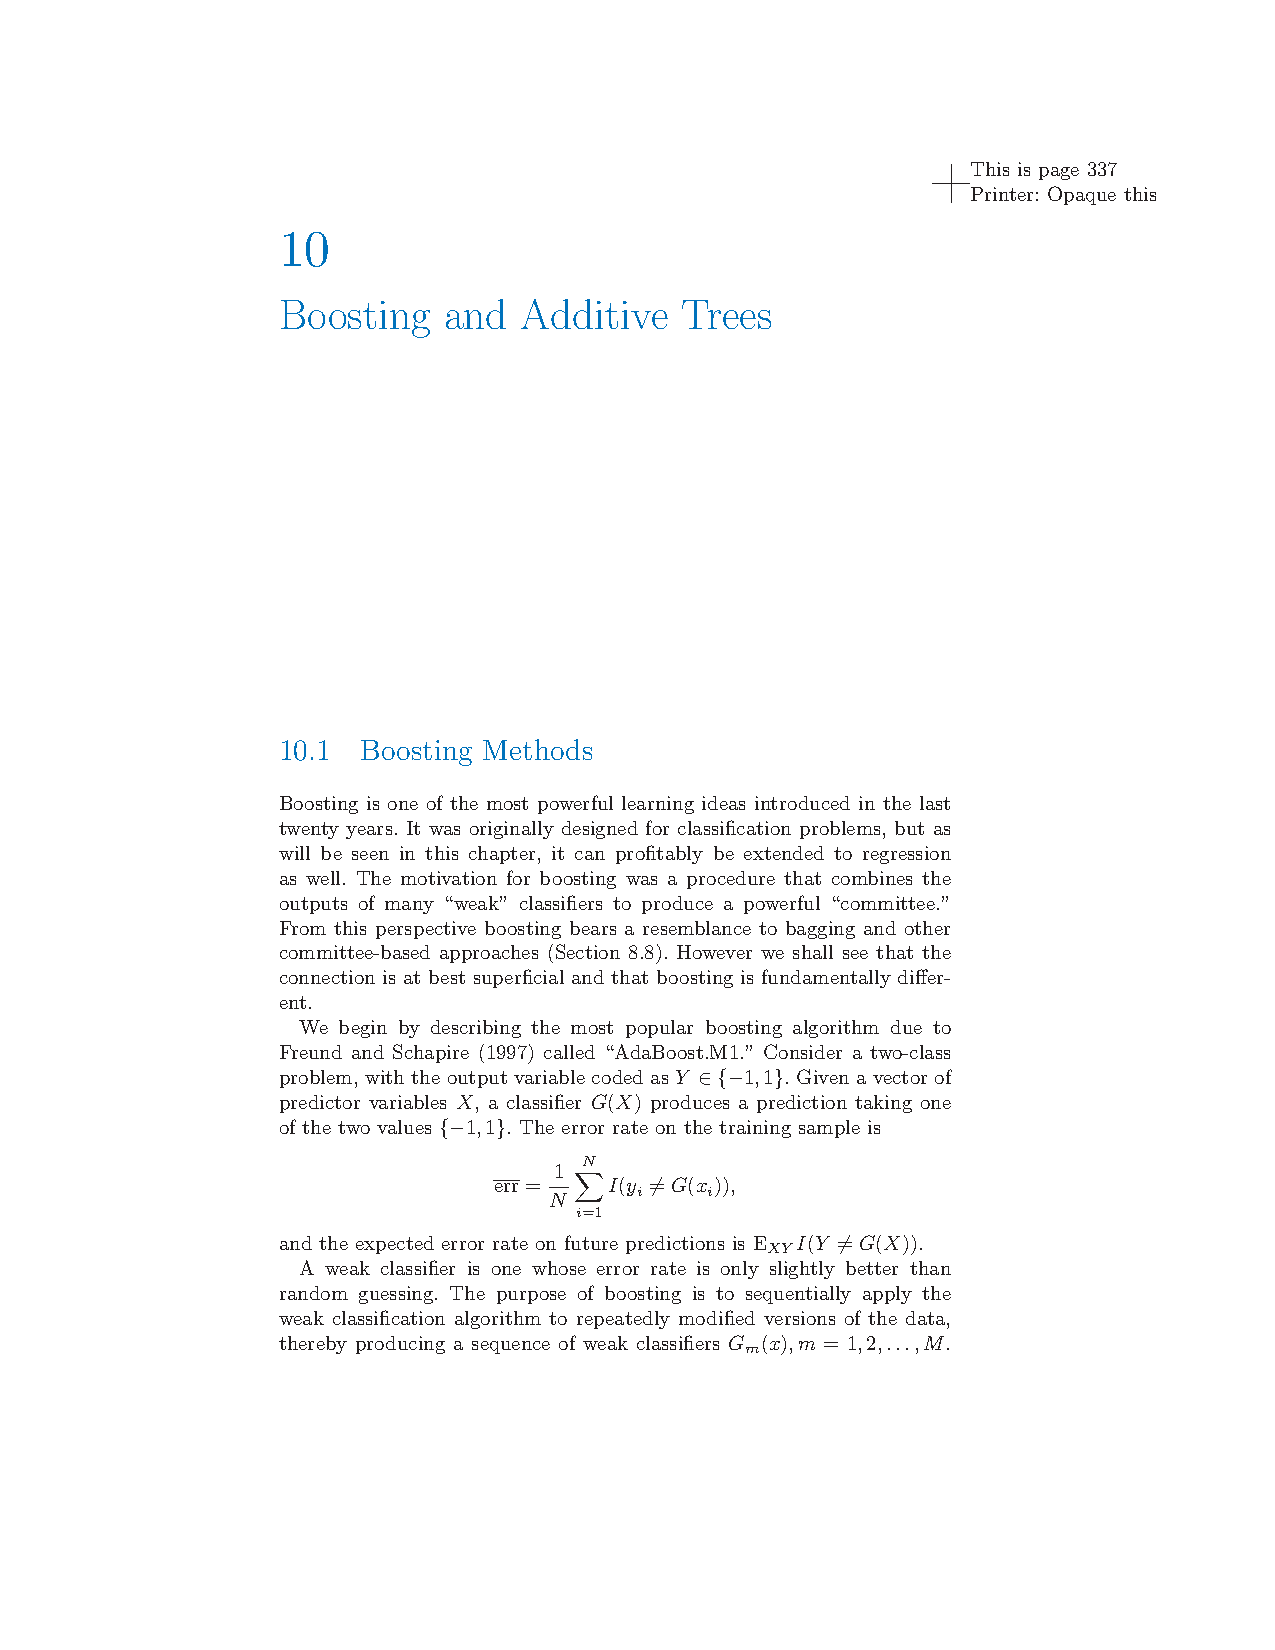
\includepdf[pages=-]{tex/boosting.pdf}
\chapter{Bagging}\label{Chapter10} 
% chktex-file 8
% chktex-file 12
% chktex-file 13
% chktex-file 44

\section{Introducción}

El \textit{bootstrap} es una herramienta estadística muy poderosa de de gran aplicabilidad que sirve para cuantificar la incertidumbre asociada a un estimador o modelo de aprendizaje estadístico dado. Se utiliza en muchas situaciones en las que es difícil o incluso imposible calcular directamente la desviación estándar de una cantidad de interés. Vemos aquí que el bootstrap puede usarse con el fin de mejorar métodos de aprendizaje estadístico como los árboles de decisión. \\

Los árboles de decisión discutidos en el el capítulo \ref{Chapter6} sufren de alta varianza (si los hacemos crecer mucho, tenemos un modelo de alta varianza y bajo sesgo). Esto significa que si dividimos los datos de entrenamiento en dos partes al azar y ajustamos un árbol de decisión a ambas mitades, los resultados que obtenemos podrían ser bastante diferentes. En contraste, un procedimiento con baja varianza ofrecerá resultados similares si se aplica repetidamente a conjuntos de datos distintos; la regresión lineal tiende a tener baja varianza (si la proporción de $n$ a $p$ es moderadamente grande). La agregación, \textit{bootstrap}, o \textit{bagging}, es un procedimiento de propósito general para reducir la varianza de un método de aprendizaje estadístico particularmente útil y frecuentemente en el contexto de los árboles de decisión. \\

Dado un conjunto de $n$ observaciones independientes $Z_1, \ldots, Z_n$, cada una con varianza $\sigma^2$, la varianza de la media $\overline{Z}$ de las observaciones está dada por 
\begin{equation}
\sigma^2/n
\end{equation}

Es decir, promediar un conjunto de observaciones reduce la varianza. Por lo tanto, una forma natural de reducir la varianza y, por tanto, aumentar la precisión de predicción de un método de aprendizaje estadístico, es tomar muchos conjuntos de entrenamiento de la población, construir un modelo de predicción separado utilizando cada conjunto de entrenamiento, y promediar las predicciones resultantes. En otras palabras, podríamos calcular $\hat{f}_1(x)$, $\hat{f}_2(x)$, \ldots, $\hat{f}_B(x)$ usando $B$ conjuntos de entrenamiento separados, y promediarlos para obtener un único modelo de aprendizaje estadístico de baja varianza, dado por
\begin{equation}
\hat{f}_{\text{avg}}(x) = \frac{1}{B} \sum_{b=1}^{B} \hat{f}_b(x).
\end{equation}

Por supuesto, esto no es práctico porque generalmente no tenemos acceso a múltiples conjuntos de entrenamiento. En su lugar, podemos usar el \textit{bootstrap}, tomando muestras repetidas del conjunto de datos de entrenamiento (único), es decir, muestrear con remplazamiento: algunos ejemplos pueden no estar presentes en el conjunto de entrenamiento, y otros pueden estar duplicados, triplicados, etc. En este enfoque, generamos $B$ conjuntos de datos de entrenamiento \textit{bootstrap} diferentes (un \textit{bootstrap} para cada árbol del bosque). Luego entrenamos nuestro método en el conjunto de entrenamiento \textit{bootstrap} $b$ para obtener $\hat{f}^*_b(x)$, y finalmente promediamos todas las predicciones, para obtener
\begin{equation}
\hat{f}_{\text{bag}}(x) = \frac{1}{B} \sum_{b=1}^{B} \hat{f}^*_b(x).
\end{equation}

\noindent Esto se llama \textit{bagging}. \\

Mientras que el \textit{bagging} puede mejorar las predicciones para muchos métodos de regresión, es particularmente útil para los árboles de decisión, ya que tienen un \textit{bias} relativamente bajo si los dejamos crecer lo suficiente. Para aplicar \textit{bagging} a árboles de regresión, simplemente construimos $B$ árboles de regresión usando $B$ conjuntos de entrenamiento \textit{bootstrap}, y promediamos las predicciones resultantes. Estos árboles se crecen profundamente y no se podan. Por lo tanto, cada árbol individual tiene alta varianza, pero bajo sesgo. Promediar estos $B$ árboles reduce la varianza. El \textit{bagging} ofrece grandes mejoras en la precisión al combinar cientos o incluso miles de árboles en un solo procedimiento. \\

Hasta ahora, hemos descrito el procedimiento de bagging en el contexto de regresión, para predecir un resultado cuantitativo $Y$. Para extender el \textit{bagging} a un problema de clasificación donde $Y$ es cualitativo, el enfoque más sencillo es el siguiente. Para una observación de prueba dada, podemos registrar la clase predicha por cada uno de los $B$ árboles, y tomar una mayoría de votos: la predicción general es la clase que ocurre con mayor frecuencia entre las $B$ predicciones. Las predicciones que daremos serán: 
\begin{itemize}
\item Regresión: 
\begin{equation}
\hat{f}_{\text{bag}}(x) = \frac{1}{B} \sum_{b=1}^{B} \hat{f}^*_b(x)
\end{equation}
\item Clasificación. Sea $\hat{f}_{\text{bag}} (x)$ la proporción de árboles que predice cada clase, se toma la probabilidad media para cada clase:
\begin{equation}
\hat{G}_{\text{bag}}(x) = \text{argmax}_k \hat{f}_{\text{bag}} (x)
\end{equation}
\end{itemize}

\begin{figure}[h]
\centering
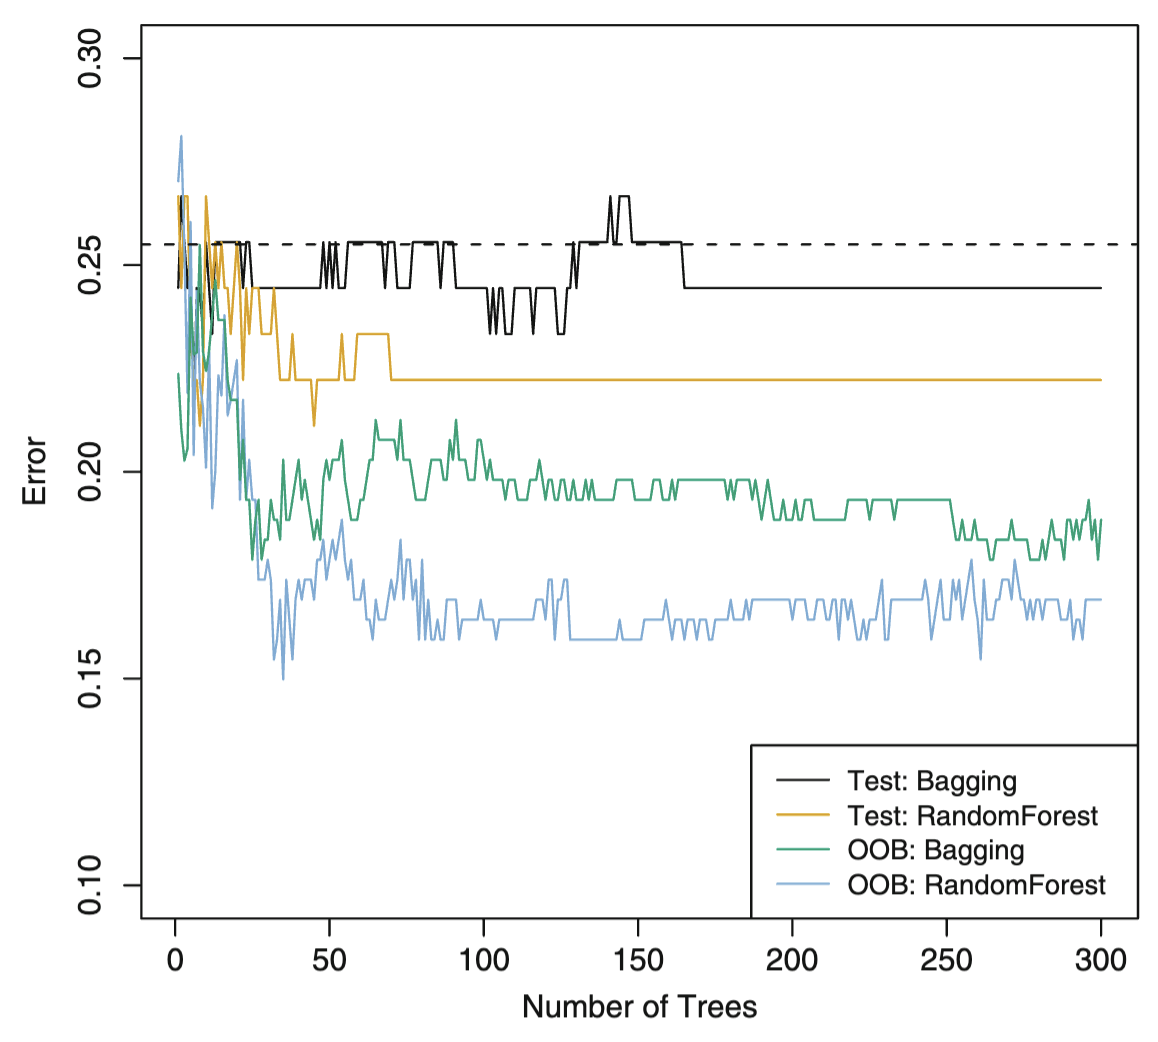
\includegraphics[width=0.5\textwidth]{fotos/59.png}
\caption{\textit{Bagging} y \textit{Random Forests} sobre los datos de \texttt{Heart}. El error de prueba (negro y naranja) se muestra como función de $B$, el número de conjunto de entrenamiento de \textit{bootstrap} usados. Se aplicaron \textit{Random Forest} con $m = \sqrt{p}$. La línea discontinua indica el error de prueba resultante de un único árbol de clasificación. Las líneas azul y verde muestran el error OOB, que resulta considerablemente menor en este caso. }
\label{fig:20.8}
\end{figure}

La figura 8.8 muestra los resultados del bagging de árboles en los datos de Heart. El número de árboles $B$ no es un parámetro crítico con el bagging; usar un valor muy grande de $B$ no llevará al sobreajuste. En la práctica, usamos un valor de $B$ suficientemente grande para que el error se haya estabilizado. Usar $B = 100$ es suficiente para lograr un buen rendimiento en este ejemplo.

\section{Random Forest}

Como ya comentamos, el \textit{bagging} parece funcionar especialmente bien para procedimientos de alta varianza y bajo sesgo, como los árboles. Para la regresión, simplemente ajustamos el mismo árbol de regresión muchas veces a versiones de los datos de entrenamiento muestreados por \textit{bootstrap}, y promediamos el resultado. Para la clasificación, un comité de árboles emite un voto para la clase predicha. \\

El \textit{boosting} se propuso inicialmente como un método de comité, aunque a diferencia del \textit{bagging}, el comité de aprendices débiles evoluciona con el tiempo, y los miembros emiten un voto ponderado. El \textit{boosting} parece dominar al bagging en la mayoría de los problemas, y se convirtió en la opción preferida. Los \textit{random forests} son una modificación sustancial del \textit{bagging} que construye una gran colección de árboles desacoplados y luego los promedia. En muchos problemas, el desempeño de los \textit{random forests} es muy similar al del \textit{boosting}, y son más sencillos de entrenar y ajustar. Como consecuencia, los \textit{random forests} son populares. 

\subsection{Definición}

La idea esencial en el \textit{bagging} es por tanto promediar muchos modelos ruidosos pero con bajo sesgo, y así reducir la varianza. Los árboles son candidatos ideales para el \textit{bagging}, ya que pueden capturar estructuras de interacción complejas en los datos y, si se crecen lo suficientemente profundos, tienen un sesgo relativamente bajo. Dado que los árboles son ruidosos, se benefician enormemente del promediado. Además, dado que cada árbol generado en el \textit{bagging} está identicamente distribuido (i.d., es decir, las muetstras de datos vienen de la misma distribución de probabilidad), la expectativa de un promedio de $B$ árboles es la misma que la expectativa de cualquiera de ellos. Esto significa que el sesgo de los árboles ``baggeados'' es el mismo que el de los árboles individuales, y la única esperanza de mejora es a través de la reducción de la varianza. Esto contrasta con el \textit{boosting}, donde los árboles se crecen de manera adaptativa para eliminar el sesgo, y por lo tanto no son i.d. \\

\noindent El \textit{random forest} introduce una aleatoriedad en el entrenamiento de cada árbol, para mantener baja la correlación y evitar el aumento de varianza. Tanto para clasificación como para regresión, sigue el siguiente proceso:
\begin{itemize}
\item Desde $b = 1$ hasta $B$:
\begin{itemize}
\item Dibuja una muestra de \textit{bootstrap} $Z^*$ de tamaño $N$ a partir de los datos de entrenamiento.
\item Crece un árbol de \textit{random forest} $T_b$ con los datos de \textit{bootstrap} siguiendo de forma iterativa los siguiente pasos para cada nodo terminal del árbol, hasta alcanzar el tamaño mínimo de nodo $n_{\text{min}}$:
\begin{itemize}
\item Selecciona $m$ variables al azar de las $p$ variables.
\item Escoge la mejor variable/punto de división entre las $m$.
\item Divide el nodo en dos nodos hijo.
\end{itemize}
\end{itemize}
\item Da como salida el conjunto (\textit{ensemble}) de árboles $\{T_b\}_{b=1}^B$.
\end{itemize}

\noindent Para hacer una predicción sobre un nuevo punto $r$: 
\begin{itemize}
\item Regresión:
\begin{equation}
\hat{f}_{\text{rf}}^B(x) = \frac{1}{B} \sum_{b=1}^{B} T_b(x)
\end{equation}
\item Clasificación: Sea $\hat{C}_b (x)$ la clase predicha por el árbol b-ésimo de \textit{random forest}. Entonces
\begin{equation}
\hat{C}_{\text{rf}}^B(x) = \text{voto mayoritario} \left\{ \hat{C}_b(x) \right\}_{b = 1}^B
\end{equation}
\end{itemize}

Para clasificación, promediamos el vector de probabilidad de cada árbol tenemos una estimación más fiable que con un voto mayoritario simple, ya que no es lo mismo que una clase gane con 0.5 que con 0.9. 
\begin{example}
Tomamos la decision con este vector promediado, no con la votacion mayoritaria.
\begin{table}[H]
\centering
\begin{tabular}{cccc}
\toprule
 & \textbf{Clase 1} & \textbf{Clase 2} & \textbf{Clase 3} \\
\midrule
\textbf{Árbol 1} & 0.5 & 0.3 & 0.2 \\
\textbf{Árbol 2} & 0.3 & 0.3 & 0.4 \\
\textbf{Árbol 3} & 0.4 & 0.1 & 0.5 \\
\midrule
\textbf{Promedio} & 0.4 & 0.23 & 0.37 \\
\bottomrule
\end{tabular}
\end{table} 
\end{example}

Una ventaja frente a \textit{boosting} es que aqui podemos paralelizar completamente el aprendizaje, ya que cada árbol se entrena de forma independiente, no como en \textit{boosting} que se entrena de forma secuencial. Otra ventaja: no hay que usar un conjunto de validación para conocer el error: el error de \textit{out-of-bag} es una estimación no sesgada del error de prueba. \\

Por tanto, al usarse para clasificación, el \textit{random forest} obtiene un voto de cada árbol y clasifica usando la clase más votada. Al usarse para regresión, la predicción de cada árbol se promedia. Además, generalmente se suelen usar los siguiente valores para el número de variables a escoger $m$ y el tamaño mínimo de nodo $n_{\text{min}}$:
\begin{itemize}
\item Clasificación: $m = \lfloor\sqrt{p}\rfloor$ y $n_{\text{min}} = 1$.
\item Regresión: $m = \lfloor p/3\rfloor$ y $n_{\text{min}} = 5$.
\end{itemize}

Un promedio de $B$ variables aleatorias i.i.d., cada una con varianza $\sigma^2$, tiene una varianza de $\frac{1}{B} \sigma^2$. Si las variables son simplemente i.d. (idénticamente distribuidas, pero no necesariamente independientes) con correlación positiva por pares $\rho$, la varianza del promedio es
\begin{equation}
\frac{\rho \sigma^2 + (1 - \rho)}{B} \sigma^2
\label{eq:15.1}
\end{equation}

\begin{itemize}
\item Para árboles i.i.d., la correlación $\rho = 0$ y la varianza se reduce a $\sigma^2/B$. Esto ocurre al principio cuando hay pocos árboles.
\item Para árboles altamente correlacionados, $\rho \approx 1$, y la varianza del modelo total tiende a $\sigma^2$, lo que significa que no hay reducción de varianza.
\end{itemize}

A medida que $B$ aumenta, el segundo término desaparece, pero el primero permanece y, por lo tanto, el tamaño de la correlación de pares de árboles ``baggeados'' limita los beneficios del promediado (es decir, se reduce la varianza, pero hasta un límite). La idea en los \textit{random forests} es mejorar la reducción de varianza del \textit{bagging} al reducir la correlación entre los árboles, sin aumentar demasiado la varianza. Esto se logra en el proceso de crecimiento de los árboles mediante la selección aleatoria de las variables de entrada. Específicamente, al crecer un árbol en un conjunto de datos bootstrap, antes de cada división, seleccionamos $m \leq p$ de las variables de entrada al azar como candidatas para la división. Generalmente, los valores para $m$ son $\sqrt{p}$ o incluso tan bajos como 1.\\

Después de que crecer $B$ árboles $\{T(x; \Theta_b)\}_{b=1}^B$, el predictor del \textit{random forest} (regresión) es
\begin{equation}
\hat{f}_{\text{rf}}(x) = \frac{1}{B} \sum_{b=1}^{B} T(x; \Theta_b)
\label{eq:15.2}
\end{equation}

$\Theta_b$ caracteriza el $b$-ésimo árbol del \textit{random forest} en términos de variables de división, puntos de corte en cada nodo, y valores de los nodos terminales. Intuitivamente, reducir $m$ reducirá la correlación entre cualquier par de árboles en el conjunto, y por lo tanto, según (\ref{eq:15.1}), reducirá la varianza del promedio. \\

\begin{figure}[h]
\centering
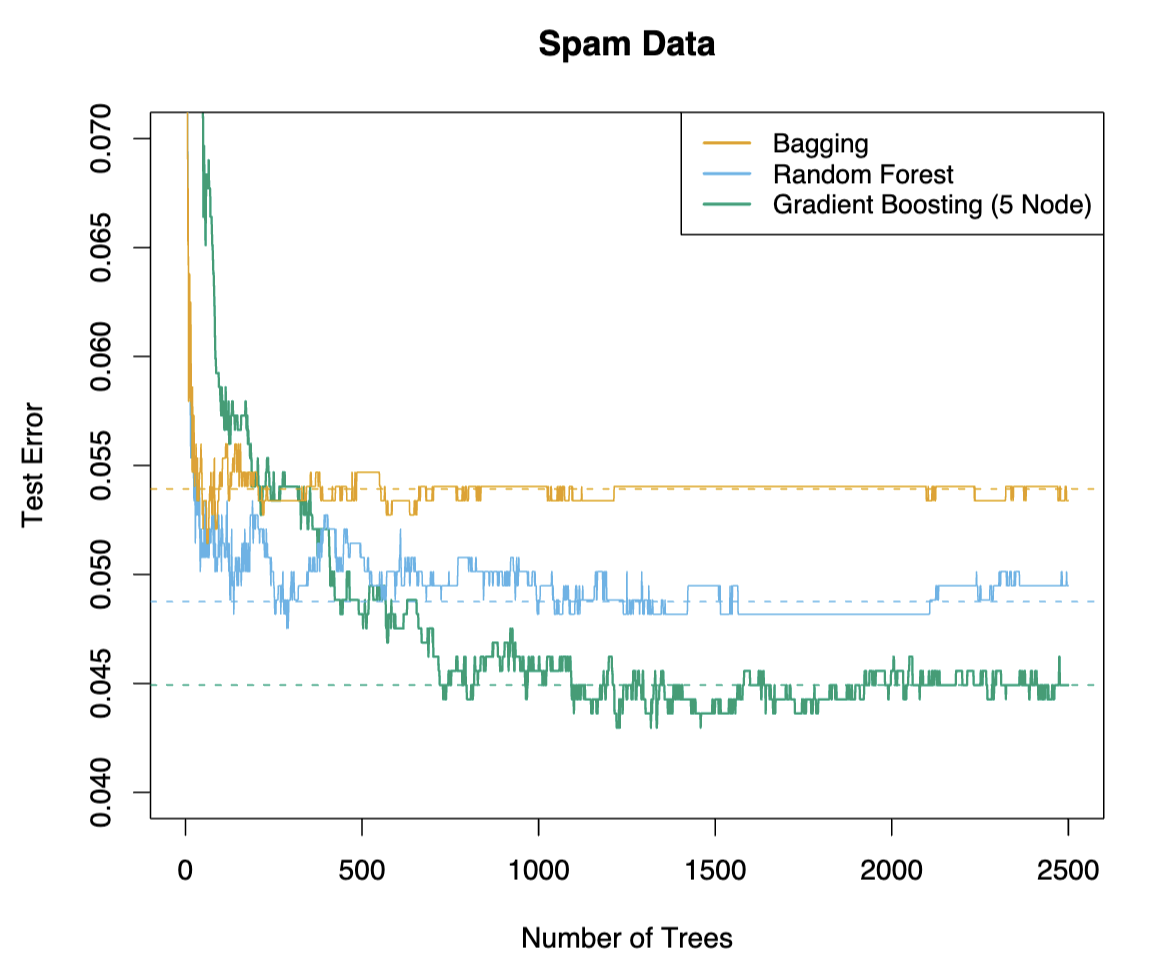
\includegraphics[width=0.5\textwidth]{fotos/60.png}
\caption{\textit{Bagging}, \textit{random forest} y \textit{gradient boosting} en el conjunto de datos de \texttt{Spam}. Para \textit{boosting} se usaron árboles de 5 nodos, y el número de árboles se escogió por validación cruzada con 10 pliegues (2500 árboles). Cada paso en la figura corresponde a el cambio en una única mala clasificación (en un conjunto de prueba de 1536 observaciones).}
\label{fig:20.9}
\end{figure}

No todos los estimadores pueden mejorarse agitando los datos de esta manera. Parece que los estimadores altamente no lineales, como los árboles, se benefician más. Para los árboles \textit{bootstrap}, $\rho$ es típicamente pequeño (generalmente 0.05 o menor; ver Figura 15.9), mientras que $\sigma^2$ no es mucho mayor que la varianza del árbol original. Por otro lado, el \textit{bagging} no cambia las estimaciones lineales, como la media muestral (y por lo tanto su varianza tampoco); la correlación por pares entre medias bootstrap es de aproximadamente 50\%. 

\subsection{Muestras \textit{out of bag}}

Una característica importante de los \textit{random forests} es el uso de muestras \textit{out-of-bag} (OOB): para cada observación $z_i = (x_i, y_i)$, se construye su predictor de \textit{random forest} promediando únicamente aquellos árboles correspondientes a muestras \textit{bootstrap} en las que $z_i$ no apareció (ya que de forma natural, \textit{bootstrap} excluye algunas observaciones). \\

Una estimación de error OOB es casi idéntica a la obtenida mediante validación cruzada de $N$ pliegues. Por lo tanto, a diferencia de muchos otros estimadores no lineales, los \textit{random forests} pueden ajustarse en una sola secuencia, realizando la validación cruzada en el camino. Una vez que el error OOB se estabiliza, el entrenamiento puede terminarse. La figura \ref{fig:20.4} muestra el error de clasificación OOB para los datos de spam, comparado con el error de prueba. Aunque aquí se promedian 2500 árboles, parece por el gráfico que alrededor de 200 serían suficientes.

\begin{figure}[h]
\centering
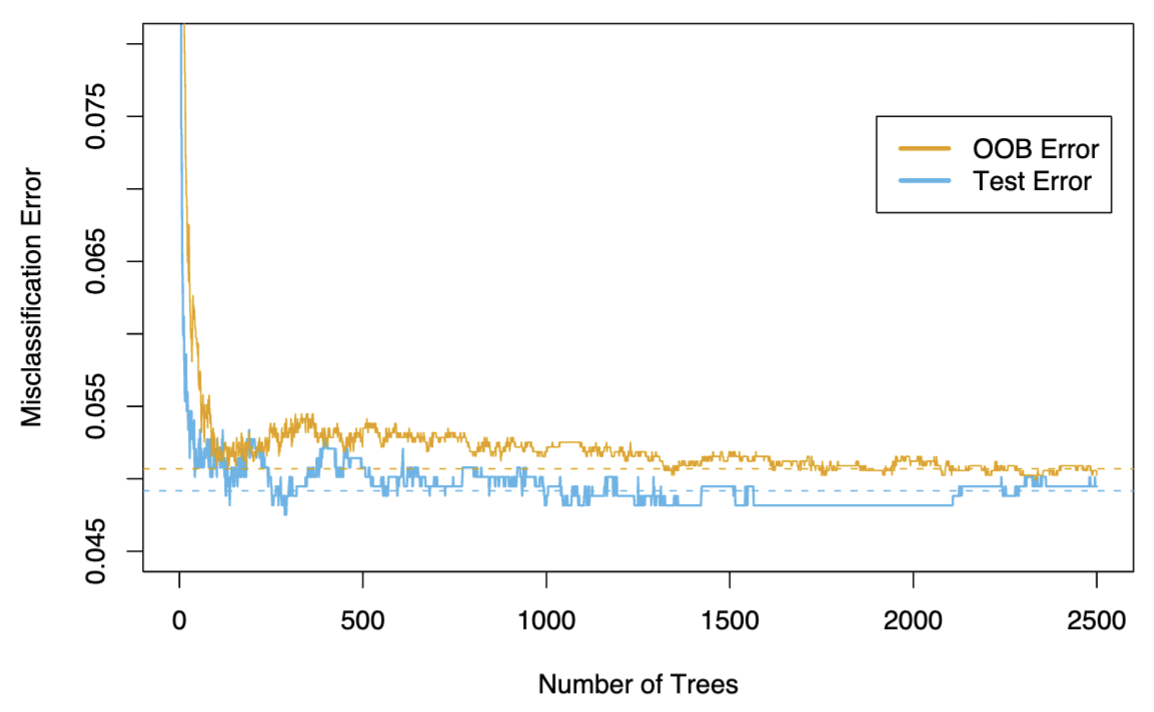
\includegraphics[width=0.5\textwidth]{fotos/61.png}
\caption{Error de clasificación OOB y error de prueba en el conjunto de datos de \texttt{Spam}.}
\label{fig:20.4}
\end{figure}


\subsection{Sobreajuste en \textit{random forest}}

Cuando el número de variables es grande, pero la fracción de variables relevantes es pequeña, es posible que los \textit{random forest} tengan un rendimiento deficiente con $m$ pequeño. En cada división, la probabilidad de que se seleccionen las variables relevantes (que den información para dar la respuesta) puede ser baja. La figura \ref{fig:20.7} muestra los resultados de una simulación que respalda esta afirmación. En la parte superior de cada par, vemos la probabilidad hipergeométrica de que una variable relevante sea seleccionada en cualquier división por un árbol de \textit{random forest} (en esta simulación, las variables relevantes son todas iguales en importancia). A medida que esta probabilidad disminuye, la brecha entre \textit{boosting} y los \textit{random forest} aumenta. Cuando el número de variables relevantes aumenta, el rendimiento de los \textit{random forest} es sorprendentemente robusto ante un incremento en el número de variables de ruido. Por ejemplo, con 6 variables relevantes y 100 de ruido, la probabilidad de que se seleccione una variable relevante en cualquier división es 0.46, asumiendo $m = \sqrt{6 + 100} \approx 10$. Según la figura \ref{fig:20.7}, esto no perjudica el rendimiento de los \textit{random forest} en comparación con el \textit{boosting}. Esta robustez se debe en gran medida a la relativa insensibilidad del costo de la mala clasificación al sesgo y la varianza de las estimaciones de probabilidad en cada árbol. Sin embargo, en un bosque esta insensibilidad se pierde, y el rendimiento de los \textit{random forest} se deteriora con el incremento del número de variables irrelevantes. \\

\begin{figure}[H]
\centering
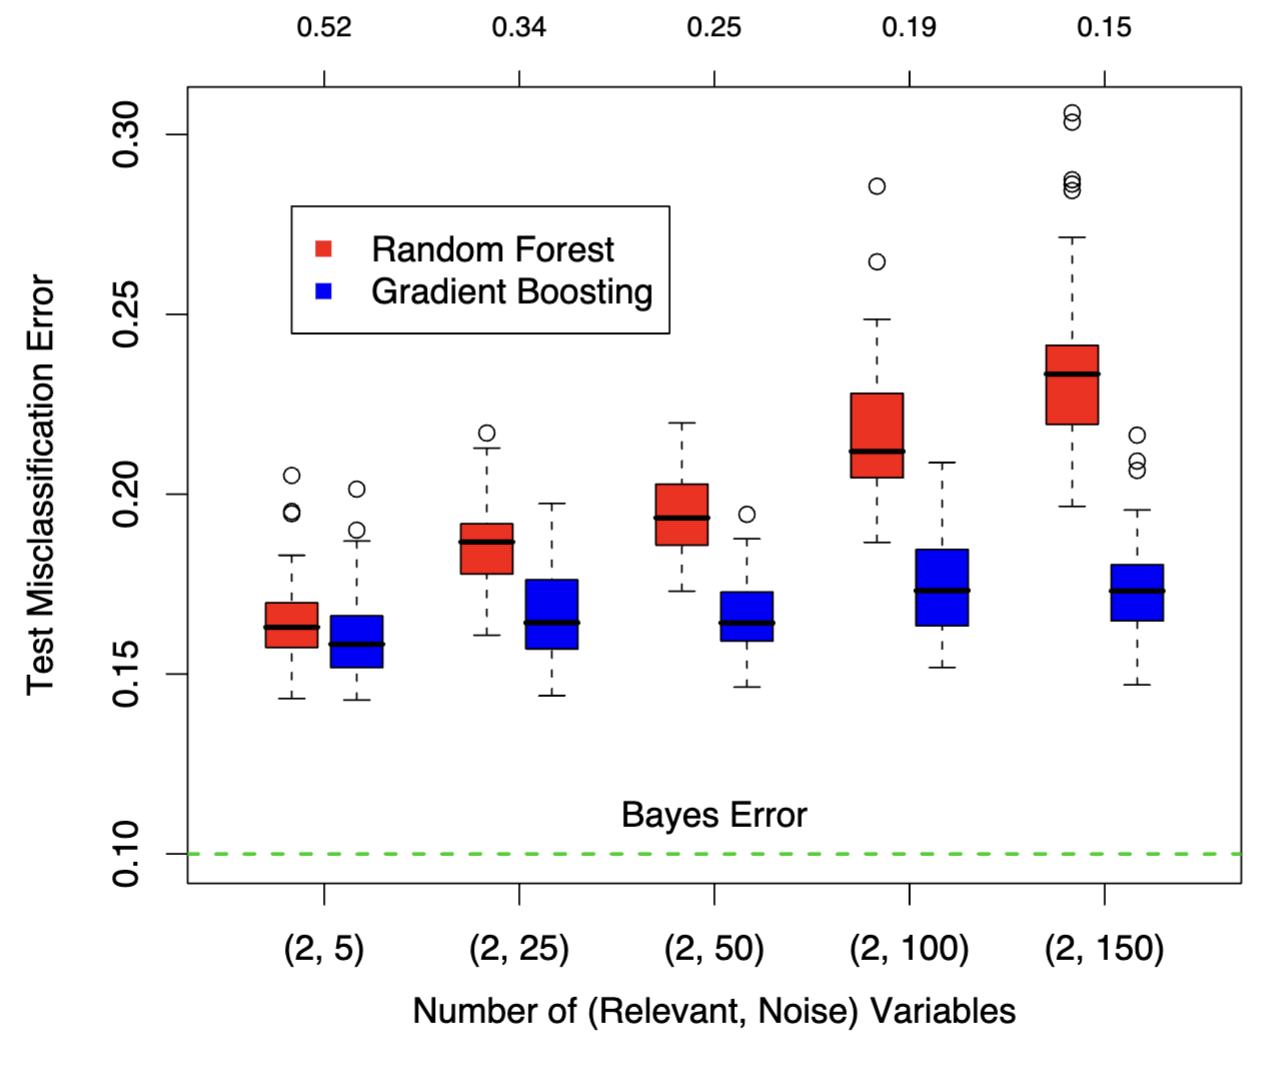
\includegraphics[width=0.5\textwidth]{fotos/62.png}
\caption{Comparación de \textit{random forest} y \textit{gradient boosting} en un problema con número creciente de variables con ruido. En cada caso, la frontera de decisión verdadera depende de dos variables, y se incluye un número creciente de variables con ruido. \textit{Random forest} usa el valor por defecto $m = \sqrt{p}$. Sobre cada par se muestra la probabilidad de elegir una variable relevante en una división o \textit{split}. Los resultados se basan en 50 simulaciones para cada par, con un conjunto de entrenamiento de 200 y un conjunto de prueba de 500.}
\label{fig:20.7}
\end{figure}

\begin{figure}[H]
\centering
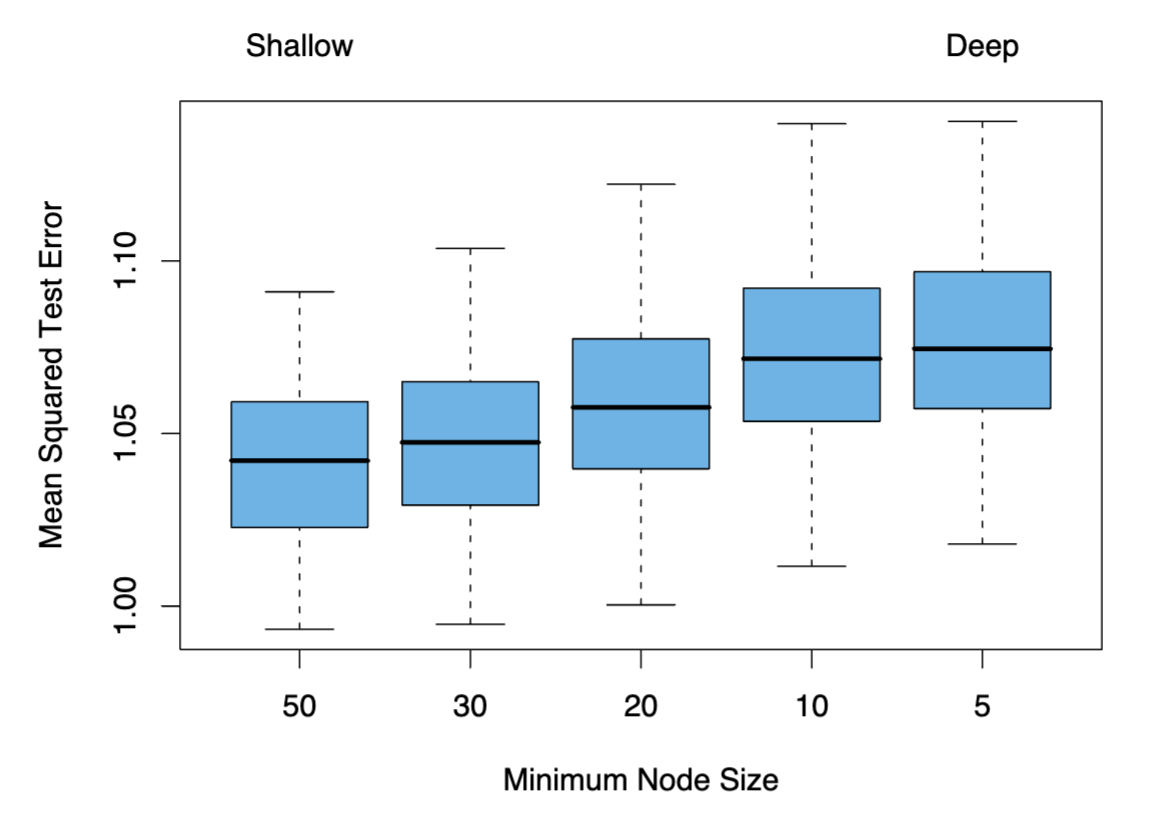
\includegraphics[width=0.5\textwidth]{fotos/63.png}
\caption{Efecto del tamaño del árbol sobre el error en regresión con \textit{random forest}. En este ejemplo, la superficie real era aditiva en 2 de las 12 variables, además de ruido gaussiano aditivo de varianza unitaria. La profundidad del árbol se controla aquí por el tamaño mínimo del nodo; cuanto menor sea el tamaño mínimo del nodo, más profundos serán los árboles.}
\label{fig:20.18}
\end{figure}

Una creencia común es que los \textit{random forest} ``no pueden sobreajustar'' los datos. Es cierto que aumentar $B$ no provoca que la secuencia de \textit{random forest} sobreajuste; al igual que el \textit{bagging}, la estimación de \textit{random forest} (\ref{eq:15.2}) aproxima la expectativa
\begin{equation}
\hat{f}_{rf} (x) = \mathbb{E}_{\Theta^T} (x; \Theta) = \lim_{B \to \infty} \hat{f} (x)_B^{rf}
\end{equation}

con un promedio sobre $B$ realizaciones de $\Theta$. La distribución de $\Theta$ aquí es condicional a los datos de entrenamiento. Sin embargo, este límite $B$ puede sobreajustar los datos si es muy grande; el promedio de árboles totalmente crecidos puede resultar en un modelo demasiado complejo, e
incurrir en una varianza innecesaria. \\

Existen pequeñas ganancias en rendimiento al controlar las profundidades de los árboles individuales cultivados en \textit{random forest}. Sin embargo, usar árboles totalmente crecidos rara vez cuesta mucho, y resulta en un parámetro de ajuste menos. Por tanto, en general, Lo normal es tratar con árboles relativamente grandes, no compensa el esfuerzo de controlar la profundidad.

La figura \ref{fig:20.18} muestra el efecto modesto del control de profundidad en un ejemplo simple de regresión. Los clasificadores son menos sensibles a la varianza, y este efecto de sobreajuste raramente se observa con la clasificación de \textit{random forest}. 




\section{18/12}


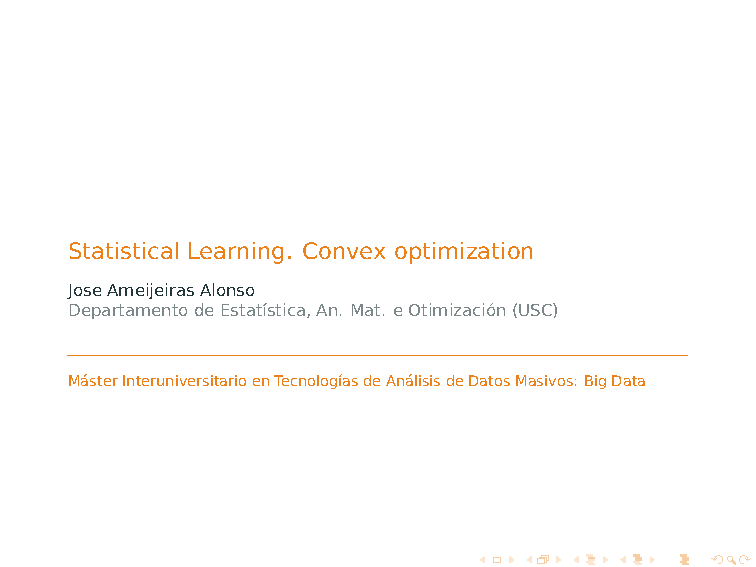
\includepdf[pages=-, nup=2x4, pagecommand={},scale=1]{/Users/luisi/Documents/Master-Big-Data/Aprendizaje estadístico/Teoría/Statistical_Learning_S3.pdf}

\end{document}  